\RequirePackage{plautopatch}
\documentclass[12pt,a4paper,report,uplatex,dvipdfmx]{jsbook}
\usepackage{mediathesis} % 卒論用パッケージ
\usepackage{listings} 

\lstset{
  basicstyle={\tiny},
  breaklines=true
}


%% Include path の設定
\graphicspath{{fig/}} %% グラフィック用
\makeatletter
\providecommand*{\input@path}{}
\g@addto@macro\input@path{{src/}}% tex ソースファイル用
\makeatother

%%%%%%%%%%%%%%%%%%%%%%%%%%%%%%%%%%%%%%%%%%%%%%%%%%%%%%%%%%%%%%%%%%%%%%%%%%%%%%%%%%%%
%%%% タイトル・概要設定 %%%%
% 提出年度(西暦)
\YearH{2021}

% 提出年(西暦)
\BringYear{2022}

% 提出月
\BringMonth{1}

% タイトル
\PaperTitle{リアルタイム 3DCG における}

% タイトル二行目(省略可)
\PaperTitleII{\LaTeX サンプルに関する研究}

% 著者名
\AuthorName{大谷真太郎}

% 学籍番号
\AuthorNumber{M01xxxxx}

% 指導教員名
\TeacherName{渡辺 大地 教授}

% 卒研プロジェクト名
\ProjectName{ゲームサイエンスプロジェクト}

% キーワード
\KeyWordsI{三次元、温度差、無礼講、}

% キーワード二行目(省略可、二行目を利用する場合は一行目の最後を読点で終わること)
\KeyWordsII{年齢差、軋轢}

% タイトル図ファイル
\TitleFig{titlems.eps}


% 概要
\Abstract{
新たな3Dプリンターの素材を開発することは,多くの人が3Dプリンターを使い新たなプロダクトを作り出し,人類の想像力を最大化させる上で重要なことだと考える.
数ある3Dプリンターの素材の中から,私は氷を素材として造形ができる3Dプリンターの開発を行った.

氷の彫刻は,世界中で様々なイベントやアート作品に用いられ,多くの人々に親しまれて様々な作品が作られている.
しかし,氷の作品は作るのには時間がかかり,彫刻の技術や設備が必要となるため,誰でも簡単に氷の造形物と触れ合えるものではない.
そのため,通常の3Dプリンターと近い操作方法で使用ができ,常温で造形が可能かつ,リアルタイムで造形が可能な氷をマテリアルとした3Dプリンターの提案をする.

世界中で使用されている3Dプリントで使用されるスライサーソフトウェアである Ultimaker Cura で操作が可能な氷をマテリアルとした3Dプリンターの開発を行った.
開発した3Dプリンターは,液体窒素で造形用ベッドを冷やすことで常温の環境下でリアルタイムに造形を行う.
また,通常の水と粘性を持たせた水ではどちらの方が氷の造形に適しているのか調査を行った.
粘性を持たせた水を使用すため,シリンダーとノズルとの距離が遠くなると,抵抗で粘性を持たせた水が通りにくくなるため,
シリンダーとノズルが直結しそこから水を絞りだす機構を開発した.

実験では,液体窒素を使い常温の環境下でリアルタイムに造形ができるかの調査と純粋な水を使用した場合と水と砂糖を1:3で混ぜた液体でどちらの方が氷の造形に適しているのか調査を行った.
今回開発した3Dプリンターの機構で常温の環境下でリアルタイムに造形することができた.
氷をマテリアルとした3Dプリンターでの造形を行う際,水と砂糖を混ぜた粘度を上げた水の方が,適しているということが分かった.
また,一般の3Dプリンターのスライサーとして広く使われているスライサーソフトUltimaker Curaを利用して造形できるため,3Dプリンターを扱えるもの方なら,少ない学習コストで使用することができる.
よって,通常の3Dプリンターと近い操作方法で使用ができ,常温で造形が可能かつ,リアルタイムで造形が可能な氷をマテリアルとした3Dプリンターを開発できた.

}


%%%%%%%%%%%%%%%%%%%%%%%%%%%%%%%%%%%%%%%%%%%%%%%%%%%%%%%%%%%%%%%%%%%%%%%%%%%%%%%%%%%%
%%%% 寸法設定 %%%%

\setlength{\textwidth}{170truemm}		% 本文横幅
\setlength{\textheight}{230truemm}		% 本文縦幅
\setlength{\topmargin}{-5truemm}		% 上部マージン調整
\setlength{\oddsidemargin}{-4truemm}		% 奇数ページ左余白
\setlength{\evensidemargin}{\oddsidemargin}	% 偶数ページ左余白
\setlength\abovecaptionskip{-0.5truemm}		% 図キャプションと図との間隔
\setlength\belowcaptionskip{1.5truemm}		% 表キャプションと表との間隔

%%%% 各種マクロ例 %%%%

\newcommand{\bez}{\mbox{$\mathrm{B \acute{e} zier}$}}
\newcommand{\dw}[2]{\mbox{$\mathrm{{#1}_{#2}}$}}
\newcommand{\uw}[2]{\mbox{$\mathrm{{#1}^{#2}}$}}

%%%% PDF ハイパーリンク各種設定 %%%%

\hypersetup{
        bookmarksnumbered=true,
        colorlinks=false,
        setpagesize=false
}


%%%%%%%%%%%%%%%%%%%%%%%%%%%%%%%%%%%%%%%%%%%%%%%%%%%%%%%%%%%%%%%%%%%%%%%%%%%%%%%%%%%%
% ここより本文開始

\begin{document}

\pagewiselinenumbers		% 行番号付加 (本番印刷の際はコメントアウト)

\MediaThesisTitle		% タイトル作成

\pagenumbering{Roman}		% 目次用ページスタイル
\tableofcontents		% 目次
\listoffigures			% 図目次(必要に応じて有効化/無効化)
%\listoftables			% 表目次(必要に応じて有効化/無効化)
\clearpage
\pagenumbering{arabic}		% 本文用ページスタイル
\pagestyle{plain}		% 本文ページ番号位置
\baselineskip=23pt		% 行間設定

% ここから本文ファイルを挿入

\chapter{はじめに}
\label{chp:first}

\section{はじめに}
\label{sec:paragraph}

3Dプリンターは2013年に低価格のものが登場するようになってから特に注目をされ続けている.
低価格化が進んだことで一般にも普及が進み2020年には3Dプリンター市場は世界で210億ドルにもなると予測されている.
3Dプリンターを活用することで製造業では,生産過程において開発期間やコストを削減することや素材の選択や高性能化ができる.
特に,これまで大量生産により,均一化された商品が一般的な社会が形成されてきたが,3Dプリンターの登場と普及により多種多様の者を少量生産ずつ,一般家庭で生産することができる.
これまで,生産者と消費者は別の者であったが,3Dプリンターの登場により生産者と消費者が同一の存在となるなりつつあるのだ. 消費者の生産者化により,これまでにない発想の商品が数多く登場し,より便利なこれまでにない発想の商品はデジタル社会により,世界中に拡散され,人類社会の発展に貢献されると考える.
3Dプリンターは人類の可能性を最大化させるためのツールでもある.その3Dプリンターは印刷できる素材が限られているのが現状である.新たな3Dプリンターの素材を開発することは,多くの人が3Dプリンターを使い新しいものを作り出し、人類の想像力を最大化させるうえで重要なことだと考える.


\section{現在の3Dプリンター}
\label{sec:paragraph}

3Dプリンターにはいくつかの種類がある.主に材料押出法,液槽光重合法,シート積層法,結合剤噴射法,材料噴射法,粉末床溶融結合法,指向性エネルギー堆積法などである.
特に一般に普及している3Dプリンターは3種類ある.
材料押出法中でも熱溶解積層方式(FDM)は,ある程度の精度(±0.1~0.2㎜程度)と速度を有し,近年では3万円以下と低価格で一般にもっとも普及している.
機構は,プラスチックのマテリアルを加熱し細いノズルから押し出して層を積み上げ造形物を作る.
液槽光重合法(光造形法(SLA))は,最も古い3Dプリンターの積層方式で,紫外線で硬化する樹脂を使用し積層していく方法である.
一層作るごとに樹脂が固まるまで紫外線を当てるため,造形に時間がかかる,その代わりに精度の高い造形(0.05㎜程度)ができるのが特徴である.
しかし,液槽光重合法(光造形法(SLA))は,マテリアルの樹脂が高価であるとともに,造形後の掃除に手間がかかり,完成後も造形物が完全に硬化するまで紫外線を当て続ける必要がある.
粉末床溶融結合法,なかでもーザー焼結 (SLS) は,金属粉末にレーザーを当て熱で溶かすことにより積層を行う.
レーザーで熱を加えるため時間がかかるが,高い精度でオブジェクトの印刷ができる.
印刷には,金属を溶かすほどの出力の強いレーザーが必要になるためサイズやコスト,安全面を考えても一般家庭では使用が難しいのが現状である.
しかし,鋳造では再現できない,液体を通すことのできる構造を作り出せるため,新しい活用方法も模索されている.

3Dプリンターに重要とされる要素は印刷精度と印刷にかかる時間があると考える.
それぞれのプリンターがどの程度2つの要素を満たしているかを に示す.
縦の軸が精度を示し,横の軸が印刷にかかる時間を表す.表を見てわかる通り,精度を優先すると速度が落ち,速度を優先すると精度が落ちてしまう.
このように,3Dプリンターの印刷は時間と精度が反比例する.
氷の造形物を印刷するプリンターは,速度を犠牲にして正確な造形物を印刷する業務用タイプと造形を直感的に行うためのハンディータイプのみで,中間の部分が欠落している.
そこで,私は精度と速度を両立させた氷の3Dプリンターを製作した.現在広く普及しているプリンターの一部を改修することで氷造形を可能にする.

\section{氷をマテリアルとした3Dプリンター}
\label{sec:paragraph}

氷の彫刻は,世界中で様々なイベントやアート作品に用いられている.
氷は透明なその美しさと時間とともに変化し,最後には溶けてなくなる儚さから人々に親しまれており,様々な作品が作られている.
しかし,誰でも簡単に触れ合えるものではなく,氷の作品を楽しめる場所は限られているのが現状である.
その原因として氷の作品は作るのに時間がかかり,彫刻の技術や設備が必要となる.
私は誰でも簡単に思い通りの形状の氷の作品を作れるようにするため,3Dプリンターを使い氷の造形物をプリントする新しい手法を提案する.
現在の3Dプリンターによる高精度な氷造形は,20mm/h のスピードで高さ 0.1mm の積層をしていく.
この速度で氷の造形物を作るには0度以下の部屋を用意し,造形中は常に造形物の周りを低温に保っておかなければならない.
また,Suntory-3D on the RocksではCNCを使った切削のため特殊な機材と知識が必要になるため,だれもが扱えるものではない.
3Dプリンターとして開発されるだけでなく,一般の多くの人に普及させるためには精度を保ちつつ素早く造形でいるプリンターである必要がある.
私は,3Dプリンターを使う知識がある人ならば,スキルに依存せずに氷の造形物を作ることができ、現状の氷をマテリアルとした3Dプリンターよりも高速で造形のできる3Dプリンターを提案する.

\section{氷造形の提案}
\label{sec:enum}

氷の造形物をつくる試みは過去に様々の方法で試されてきた.氷をマテリアルとした自動造形には現状2パターンがある.
1つ目が氷の塊をCNCで掘削する方式である.CNC方式では,精度の高い氷をマテリアルとした造形を行おうことができるのだが,特殊な設備と技術が必要になる.
2つ目が3Dプリンターと同じ仕組みで精度の高い造形物を印刷することができるが,造形速度が20mm/hのスピードで高さ0.1mmの積層とかなり速度がかなり遅い.
これらの氷をマテリアルとした造形方法では造形速度が遅く,冷凍庫のような特殊な環境が必要になるため,一般の人が気軽に氷をマテリアルとした造形を利用することが難しいのが現状である.
氷をマテリアルとした造形物の使用用途は、現実に氷をマテリアルとした工業製品が無いのを考えると,強度的な問題や常温で溶け出す問題などにより,観賞用に用いられることがほとんどと考えられる.
使用用途が観賞用であると考えた場合、工業用製品に必要な要素が正確性(精度)などに対して,観賞用では,氷の条件を満たしたうえで一般の人でも扱いが可能かつ,一般のユーザーが設計したデータにできるだけ近い形に印刷されれば問題ないと考えられる.
また,氷を再定義する.氷をまたリアルとした3Dプリンターの主な使用用途は観賞と考える.観賞とは,氷特有の常温で液体へと徐々に変化し,最後にはなくなるこの過程が,ほかのマテリアルにはない大きな特徴であるこの部分を指すと考える.
そのため、氷の定義として下記の2つを定義する.

\begin{enumerate}
  \item 固体であるとき常温より低温であること. 
  \item 常温で溶けること.
 \end{enumerate}

氷の定義を以上のようにしたうえで,一般の人でも扱いが可能かつ,一般のユーザーが設計したデータにできるだけ近い形に印刷できる氷をマテリアルとした3Dプリンターの提案する.




		% 第1章
\chapter{関連研究}
\label{chp:first}

\section{関連研究}
\label{sec:paragraph}
新しいマテリアルを使い,今までにない3Dプリンターでは表現できなかったモノを作ることを可能にしている研究を中心最新の3Dプリンターに関する研究を調査した.


\section{ゲルを用いて印刷する3Dプリンター\cite{a}}
\label{sec:enum}

この研究は,ゲルをマテリアルとして用いた造形物を3Dプリンディングするものである.
図2.1のように,ゲル溶液を使用しながら強度や感触を部位によって変化させて造形物を作成することができる.

\begin{figure}[H]
  \centering
  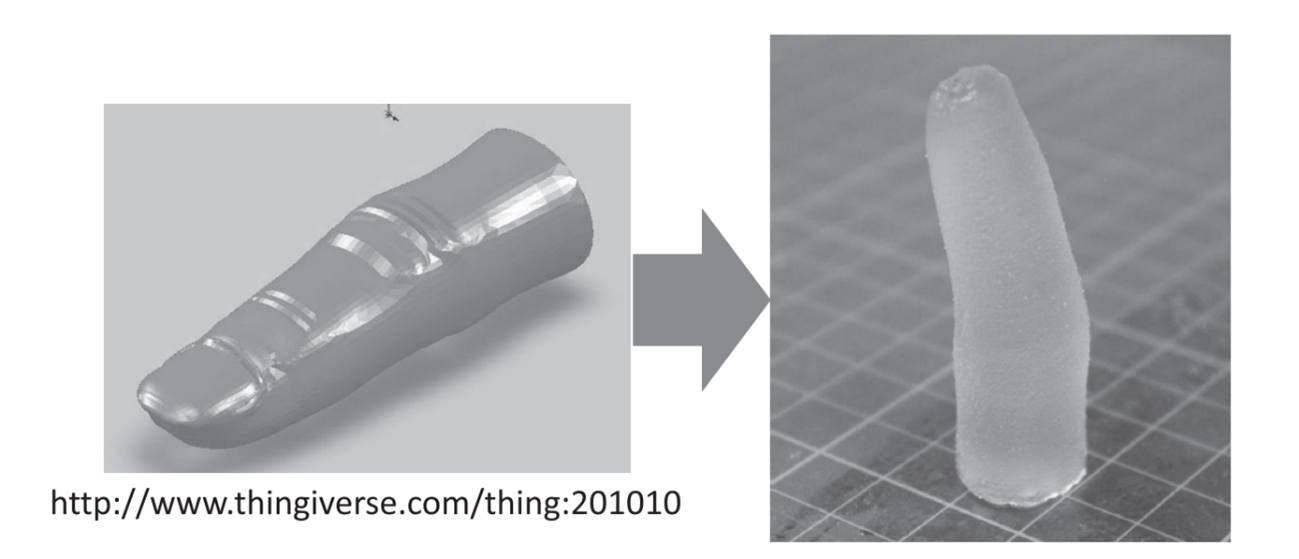
\includegraphics[width=14truecm]{./fig/geru3D.png}
  \caption{3Dゲルプリンターで作製した造形物}
% \url{http://www.this.is.sample.url/} % Web上のデータの場合、参照先URLを明記
  \label{fig:ss}
\end{figure}

これは,ゲル化を誘起するUVレーザーを光ファイバーを通して局所的にゲル溶液に照射することで,ゲルの3次元造形を可能にしている.3Dプリンターは現在,臓器の立体イメージを作り出すのに医療分野で活用されているが,手術の計画や事前検証のための立体の臓器モデルを作製するには,数千万もする工学な3Dプリンターを使用してプラスチックやゴムなどの,実際の臓器よりもはるかに硬い樹脂を用いて造形をする方法しか存在しなかった.
このゲルを用いて印刷する3Dプリンターは,低コストで感触がより患者のものと似ている臓器モデルを作成できる可能性を秘めている.

この3Dプリンターは材料として微粒子調整ダブルネットワークゲル(略称:P-DNゲル)を使用している.このゲルは強電解質性を示すモノマー由来の堅く脆い高分子ネットワーク(1st ネットワーク)と,中性を示すモノマー由来の柔軟な高分子ネットワーク(2nd ネットワーク)が相互侵入網目構造をとっている複合材料である.このP-DNゲル溶液にUVレーザーを照射することでラジカル反応が生じ,ゲルの3次元構造をつくることができる.


\section{Suntory-3D on the Rocks\cite{b}}
\label{sec:enum}

氷を掘削し様々な彫刻を作りお酒に入れて楽しむ試みがある.
多軸の CNC を使い掘削することで高精度の彫刻を作ることができるが,一般に普及させるのはコストならびに加工中の冷却の面から考えると難しい.
制作の過程と実際に制作されたものを図2.2に示す.

\begin{figure}[H]
  \centering
  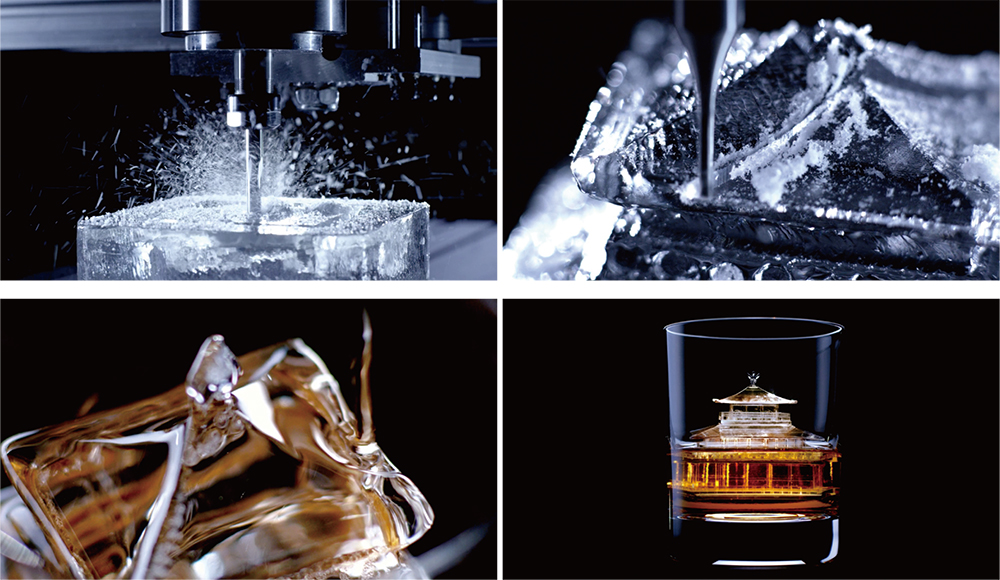
\includegraphics[width=12truecm]{./fig/Suntory.jpg}
  \caption{実際に掘削して作製した高精度の彫刻の例}
  \url{https://mag.sendenkaigi.com/brain/201406/up-to-works/002420.php} % Web上のデータの場合、参照先URLを明記
  \label{fig:Suntory}
\end{figure}


\section{A Layered Fabric 3D Printer for Soft Inter active Objects\cite{c}}
\label{sec:enum}
この研究では布の造形物を印刷するためのプリンターを紹介している.
また,布の中に導電繊維の層を入れたり,コイル状の布を入れることで,タッチセンサーとしての利用法や NFC を使い LED を光らせるアプリケーションが紹介されている.
このプリンターの仕組みは,布のロールを引き出し天板に吸着させ固定し,レーザーでモデルの輪郭を切断し布のロールから切り出す.
この工程を繰り返し,アイロンの熱で接着していくことで造形物が完成する.完成した造形物を図2.3に示す.

\begin{figure}[H]
  \centering
  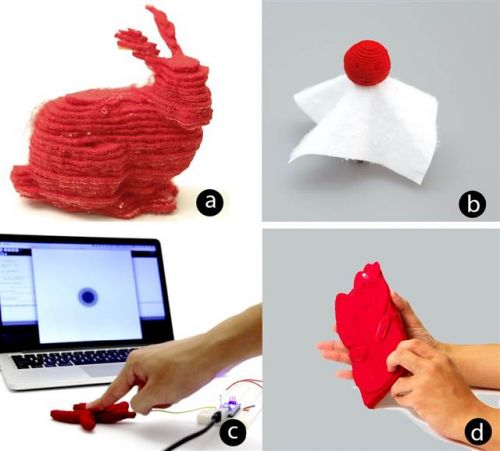
\includegraphics[width=10truecm]{./fig/ALayered.jpg}
  \caption{実際に印刷された布の造形物}
  \url{https://thelastnewspaper.com/a-layered-fabric-3d-printer-for-soft-interactive-objects/} % Web上のデータの場合、参照先URLを明記
  \label{fig:ferret}
\end{figure}



\section{ Additive manufacturing of optically trans-parent glass\cite{d}}
\label{sec:enum}
ガラスをマテリアルに使ったこの研究では,高温で流動性の高い状態に保持されたガラスを貯めておき,そのガラスを垂らすことで造形していく.
実際に造形されたガラスの造形物は1回のストロークで出せるラインは太く分厚いものであり,細かい造形はできないがサイズの大きい花瓶のようなものを造形することができる仕組みと過程を図2.4 図2.6に示す.
この手法で造形された花瓶は光を乱反射させる特性があり,上からライトを当て光の波紋を楽しむアプリケーションが図2.のように提示されていた.

\begin{figure}[H]
  \centering
  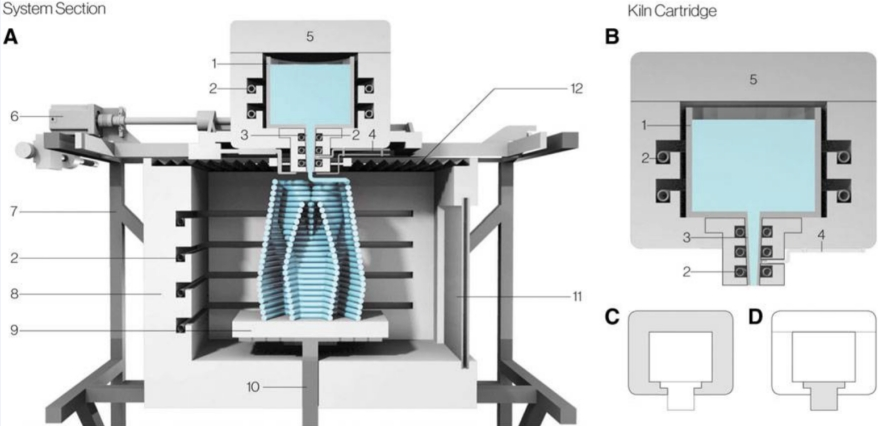
\includegraphics[width=12.5truecm]{./fig/Additive2.jpg}
  \caption{ガラス造形の仕組み}
% \url{http://www.this.is.sample.url/} % Web上のデータの場合、参照先URLを明記
  \label{fig:ferret}
\end{figure}

\begin{figure}[H]
  \centering
  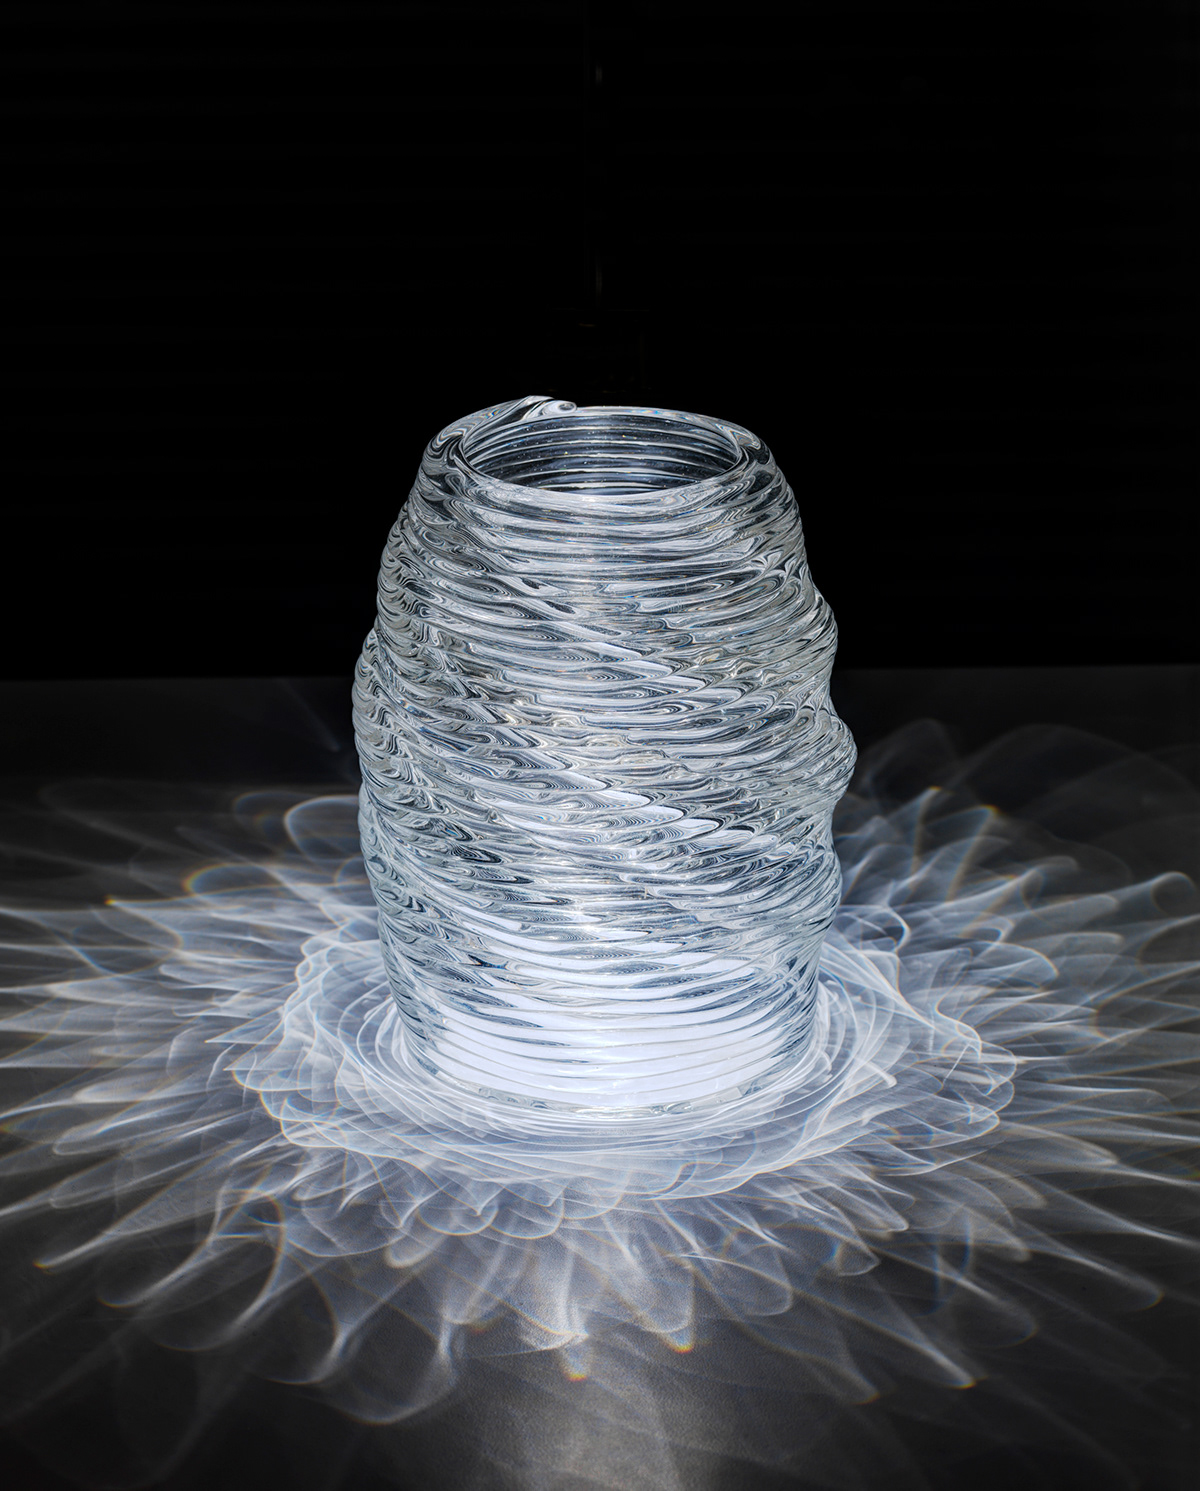
\includegraphics[width=8truecm]{./fig/Additive1.jpg}
  \caption{造形されたガラスの造形物}
  \url{https://www.behance.net/gallery/65276297/GLASS-I} % Web上のデータの場合、参照先URLを明記
  \label{fig:ferret}
\end{figure}

\begin{figure}[H]
  \centering
  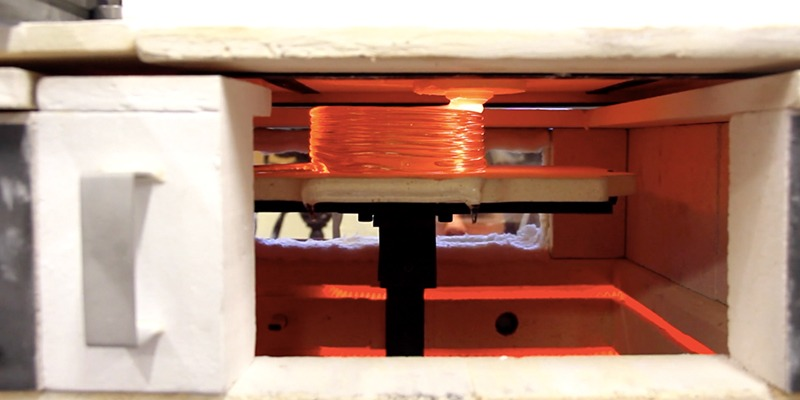
\includegraphics[width=13truecm]{./fig/Additive3.jpg}
  \caption{制作中の様子}
  \url{https://www.solidsmack.com/fabrication/mits-mediated-matter-group-unveils-transparent-glass-3d-printer/} % Web上のデータの場合、参照先URLを明記
  \label{fig:ferret}
\end{figure}


\section{静電インクジェット式3Dプリンタによる高粘度食品材料の高精度プリント\cite{e}}
\label{sec:enum}
この研究では静電インクジェット法を用いることで,高い印刷精度で高粘度材料を用いた,視覚的,味覚的に優れた食品の印刷を可能にする3Dプリンターの開発をしている.

従来の食品の3Dプリンターには熱溶解式(FDM)式3Dプリントを用いたチョコレートの印刷がある.しかし,熱溶解式では積層ピッチが約0.5[mm]以上と非常に粗く,また高粘度材料をプリントする際には添加物を加える必要がある.この添加物には,食品の味に影響が出てくる問題点がある.
静電インクジェット法を用いると,この問題を解決すると同時に高精度な印刷が可能となる.
下の図2.7の様なチョコレートプリンターを作製し,実験を行った.


\begin{figure}[H]
  \centering
  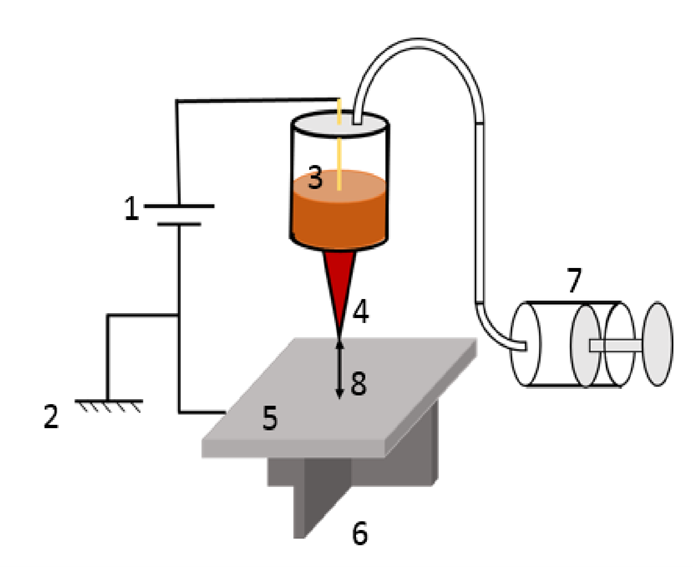
\includegraphics[width=11truecm]{./fig/seidenn.png}
  \caption{静電インクジェット式プリンターによるチョコレートプリントの仕組み}
  %\url{https://thelastnewspaper.com/a-layered-fabric-3d-printer-for-soft-interactive-objects/} % Web上のデータの場合、参照先URLを明記
  \label{fig:ferretss}
\end{figure}

この3Dプリンターは高粘度食品材料であるミルクチョコレートに高電圧を加え微小液滴を吐出し,下図2.8のような超微細なラインを印刷することを可能にする.
また電圧のコントロールによって,吐出するラインの径を制御することもできる.

\begin{figure}[H]
  \centering
  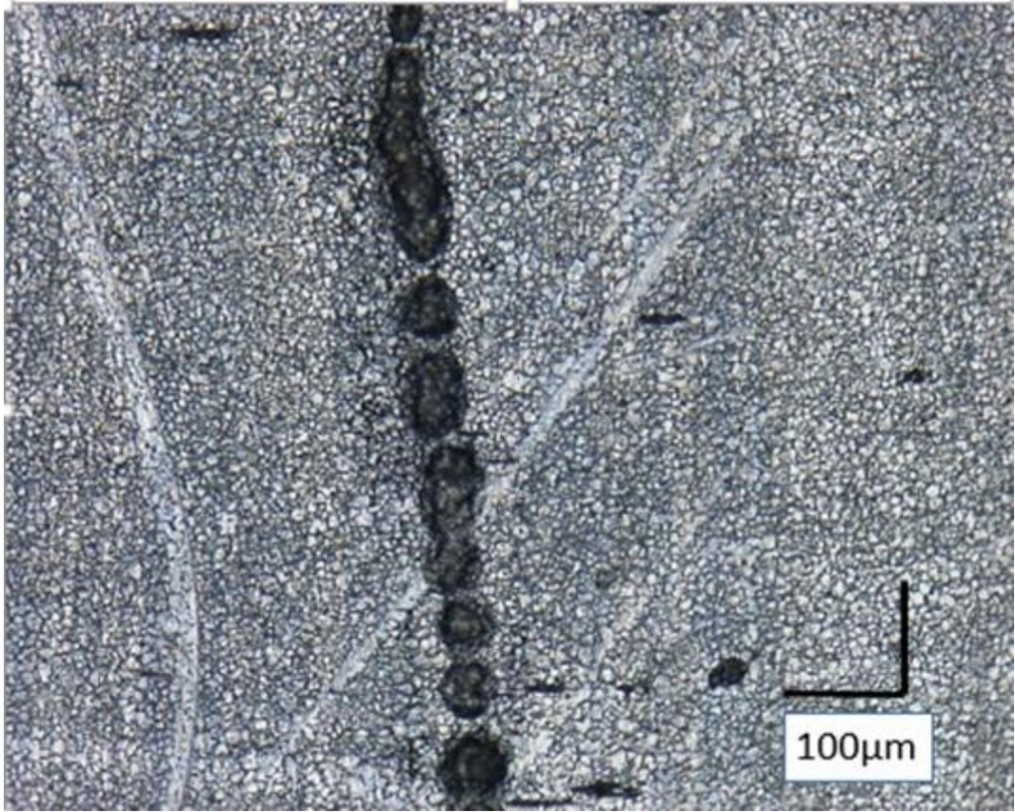
\includegraphics[width=9truecm]{./fig/seidenn2.jpg}
  \caption{実際に吐出されたチョコレートを顕微鏡を用いて観察した様子}
  %\url{https://thelastnewspaper.com/a-layered-fabric-3d-printer-for-soft-interactive-objects/} % Web上のデータの場合、参照先URLを明記
  \label{fig:ferret}
\end{figure}


\section{フルカラー3Dプリンター—2D印刷から3D印刷へ—\cite{f}}
\label{sec:enum}
フルカラー3Dプリンターについて紹介する.
このプリンターはUV(紫外線)硬化インクジェット方式を採用したことで任意の3D形状の造形を可能にすると同時に,その表面にフルカラーで印刷することができる.
このフルカラー3Dプリンターにより,クリエイターの創造物が画面の中だけではなく,今までより容易に手に取れるようになっている.
新しい市場も徐々に出現し始めていて,最近では3D撮影による人文やペットのリアルなコピー造形物が話題になっている.

この3Dプリンターは,下図2.9のようにインクをUV光源で硬化させながら積層法で造形を行う.

\begin{figure}[H]
  \centering
  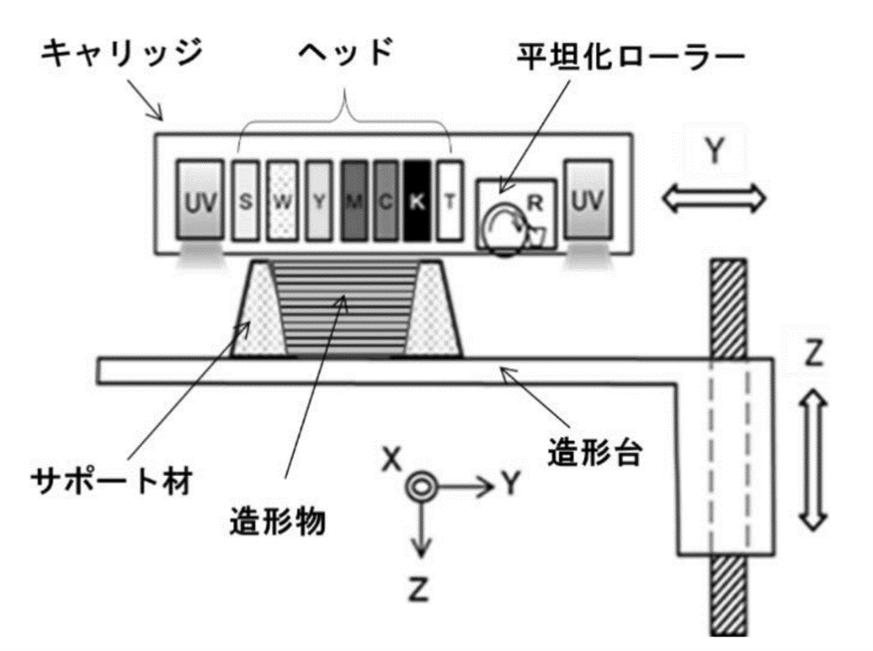
\includegraphics[width=11truecm]{./fig/hurukara.png}
  \caption{フルカラー3Dプリンターの概略図}
  %\url{https://thelastnewspaper.com/a-layered-fabric-3d-printer-for-soft-interactive-objects/} % Web上のデータの場合、参照先URLを明記
  \label{fig:ferret}
\end{figure}

2Dと3Dを比較した時,フルカラー3Dプリンターでは下図2.10のような印刷が行われている.

\begin{figure}[H]
  \centering
  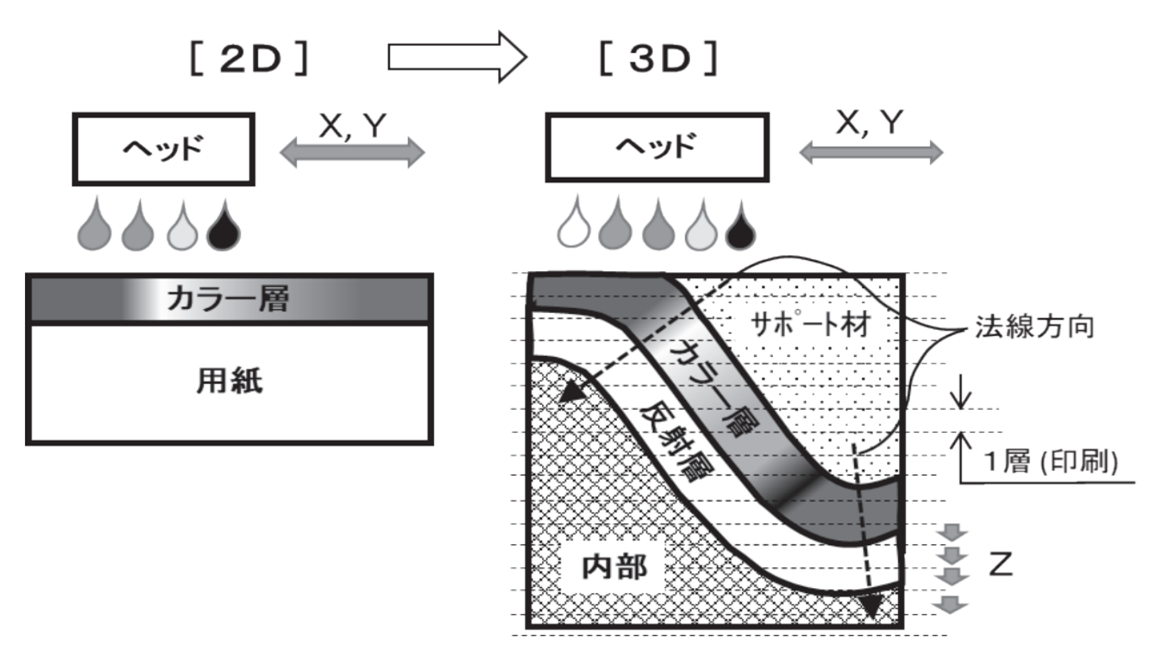
\includegraphics[width=11truecm]{./fig/hurukara2.png}
  \caption{2Dプリンターとフルカラー3Dプリンターの違い}
  %\url{https://thelastnewspaper.com/a-layered-fabric-3d-printer-for-soft-interactive-objects/} % Web上のデータの場合、参照先URLを明記
  \label{fig:ferret}
\end{figure}

2Dの印刷では画像データの濃度によりカラーインクの量が変化するが,これを3Dに適用するとカラー創の外形が崩れてしまうため,カラーインクのない空きスペースには透明インクを補填して外形を保つ工夫をしている.

\section{3D プリンタのセラミックスへの適用\cite{g}}
\label{sec:enum}
この研究では,セラミックス材料を用いた3Dプリンター開発を行っている.
主にセラミックス緻密体を作製する基礎検討に関しての研究である.

今回このプリンタには,SLM方式を採用する.
この方式では図2.11のように,薄く敷き詰めた粉末床にレーザや電子ビームを走査して粉末を溶解し,順次積層することで3次元の造形物を得る.
昨今では,レーザや電子ビームの出力向上に伴い,新規な材料の適用が可能となってきているが,セラミックスに関しては,急熱急冷を伴うプロセスの特性上衝撃熱が発生するため構造体の密度向上が難しく,工業的な部材の製造は実現していない.
この高密度焼結体の迅速な3次元造形が実現すれば,小ロットの射出成形やテープ整形の代替,複雑形状を生かした高性能セラミックスフィルターや半導体作製用の露光ステージへの利用が期待できる.

\begin{figure}[H]
  \centering
  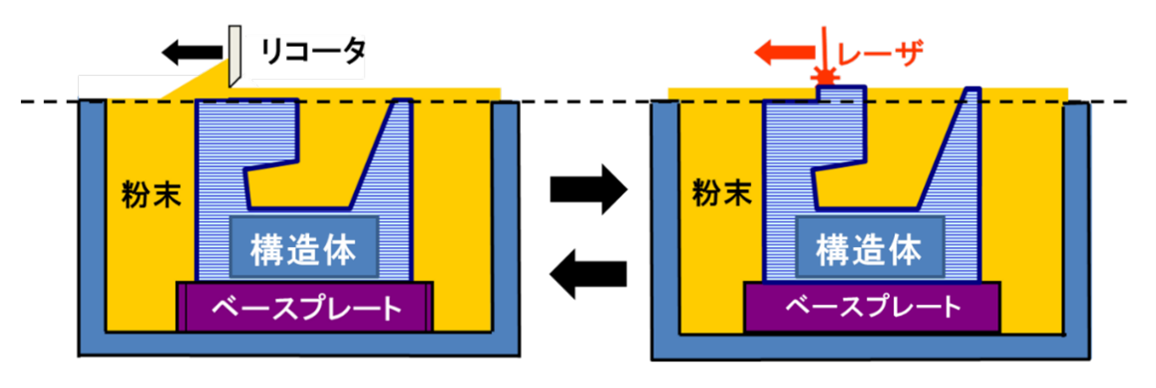
\includegraphics[width=14truecm]{./fig/seramikku1.png}
  \caption{SLM法を用いてセラミックスを印刷する際の様子の模式図}
  %\url{https://thelastnewspaper.com/a-layered-fabric-3d-printer-for-soft-interactive-objects/} % Web上のデータの場合、参照先URLを明記
  \label{fig:ferret}
\end{figure}

熱衝撃を回避したセラミックスのSLM法として,直接セラミックスを焼結せずに,レーザによる形状の作製と焼結による密度向上を分離した間接法が考案されている.この間接法では,セラミックスと低融点の樹脂成分と複合化した粉末を用い,樹脂部分のみをレーザ溶解することでシート成形,グリーン体を作製し,その後,脱脂・焼結することによりセラミックス単体の焼結体を得るものである.間接法を用いた様々な試みがなされてきたが,造形に時間がかかる,密度が低いなどの理由で工業的な利用には未だ至っていない.

この研究では,高強度アルミナ焼結体の作製を目的とした間接法プロセス構築のための検討を行い,アルミナの相対密度が94%の焼結体の作製に成功している.
検討のため,①~③のそれぞれの特性に着目した

①原料セラミックスの選定
・粒子径・粒子径分布

②原料樹脂の選定
・脱脂性・樹脂の融点またはガラス移転点

③造粒粉の作製
・流動性・粒子径・かさ密度・1個粒子の密度

その他にも,SLM条件の最適化,3Dプリンタ内の粉体挙動のシュミレーションを行った結果,以下の図2.12のような,アルミナの相対密度が94%セラミック緻密体を作製することに成功した.

\begin{figure}[H]
  \centering
  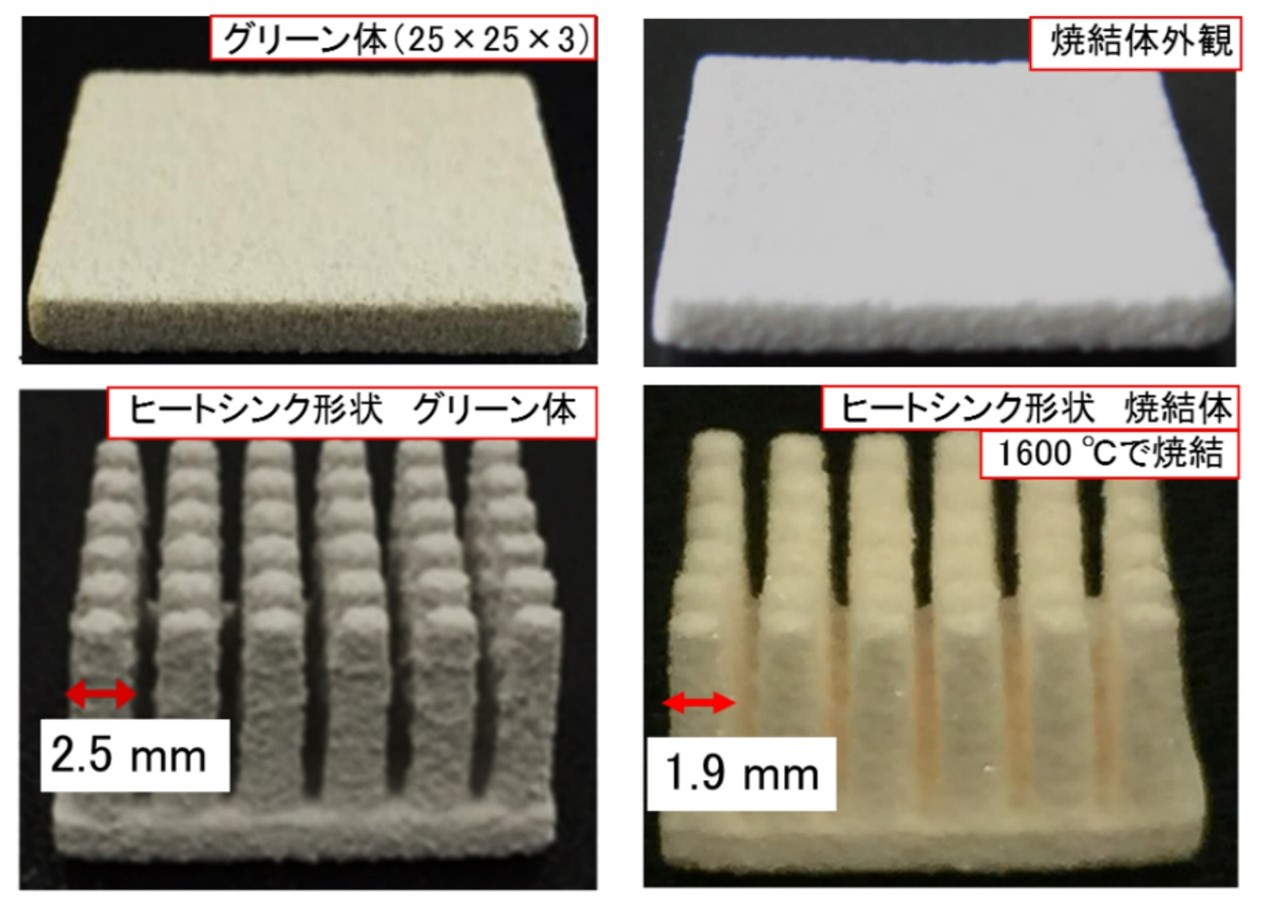
\includegraphics[width=11truecm]{./fig/seramikku.jpg}
  \caption{SLM法を用いた印刷で完成した造形物}
  %\url{https://thelastnewspaper.com/a-layered-fabric-3d-printer-for-soft-interactive-objects/} % Web上のデータの場合、参照先URLを明記
  \label{fig:ferret}
\end{figure}


\section{3D食用ゲルジェットプリンタによる食品創製\cite{i}}
\label{sec:enum}
この研究では,現代の高齢者が食事をより食べやすく,見た目も楽しめるような食品が造形できる,食用のゲルプリンタの開発をしている.

この研究で使用するゲルプリンタは図2.13のように,①搬送系,②液送系,③冷却系の,三つの機構から成り立っている.

\begin{figure}[H]
  \centering
  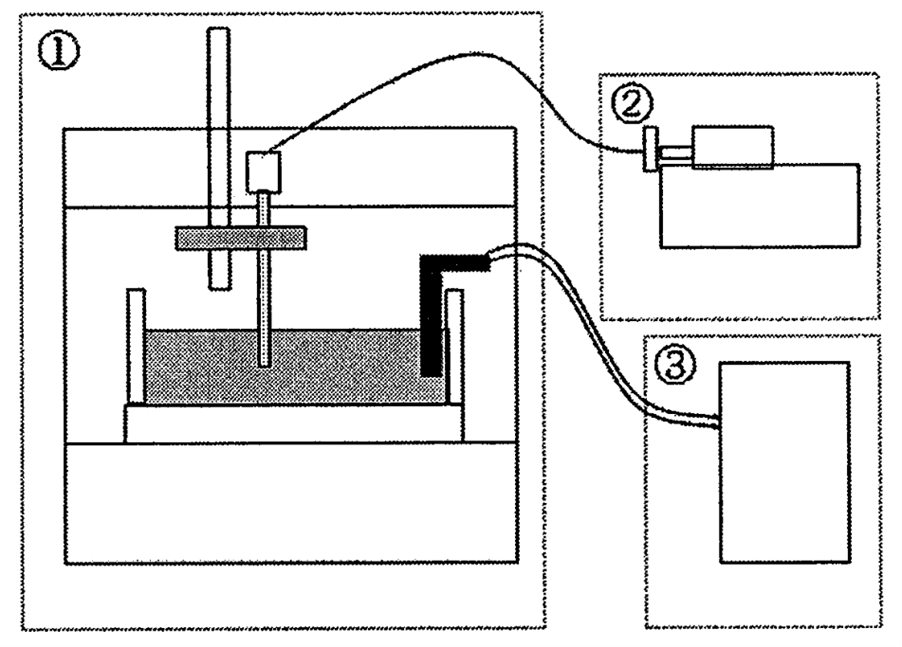
\includegraphics[width=10truecm]{./fig/geru.png}
  \caption{3D食用ゲルジェットプリンタの模式図}
  %\url{https://thelastnewspaper.com/a-layered-fabric-3d-printer-for-soft-interactive-objects/} % Web上のデータの場合、参照先URLを明記
  \label{fig:ferret}
\end{figure}

①は,②のシリンジポンプによって送り出された溶液をコンピュータ制御により,任意の形状に造形することが可能な機構である.②は,ゲルの溶液をシリンジで①の方へ押し出す機構となっている.③は,溶液を滴下する水槽を冷却する機構である.
この装置を用いることで,アルギニン酸ゲル(人工イクラ)の造形が可能となる.

またこの研究では,プリンタに使用するゲルの冷却方法の検討も行った.
寒天とゼラチンの溶液をシリンジを使用しアルミの皿に垂らしていった.1分経過後,寒天,ゼラチン共に固まったが,寒天に比べゼラチンは少し皿にくっついて剝がそうとするとボロボロになった.二つに共通し濃度が高くなると固まりやすくなる傾向があるが,その場合でもゼラチンは強く付着する傾向がある.これは,寒天とゼラチンが植物性と動物性という違いに起因するものだと考えられる.下図が寒天とゼラチンが固まった様子である.

\begin{figure}[H]
  \centering
  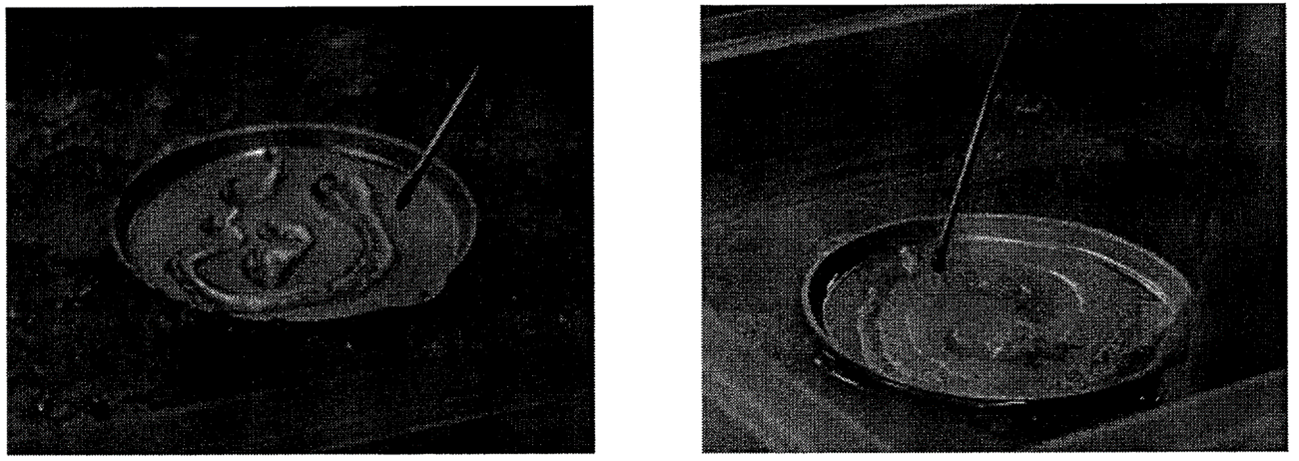
\includegraphics[width=12truecm]{./fig/geru2.png}
  \caption{寒天とゼラチンの溶液をそれぞれアルミの皿に垂らしたときの様子}
  %\url{https://thelastnewspaper.com/a-layered-fabric-3d-printer-for-soft-interactive-objects/} % Web上のデータの場合、参照先URLを明記
  \label{fig:ferret}
\end{figure}

\section{積彩\cite{h}}
\label{sec:enum}
通常の3Dプリンター特にカラー3Dプリンターでも複数の色をせきそうすることでカラー3Dプリンターとしている.
この積彩では,コンピューティングによって調色しながら色糸を積む3Dプリンティングの製造によって造形・着彩をひとつの工程として扱っている.
これを「積彩」と呼び,また,繊細な織物のように糸を積んでいく積彩は新たな表現技法(虹のように変化する色彩効果)を可能にし、この技法を応用して「色瓶」というプロダクト製作している.

\begin{figure}[H]
  \centering
  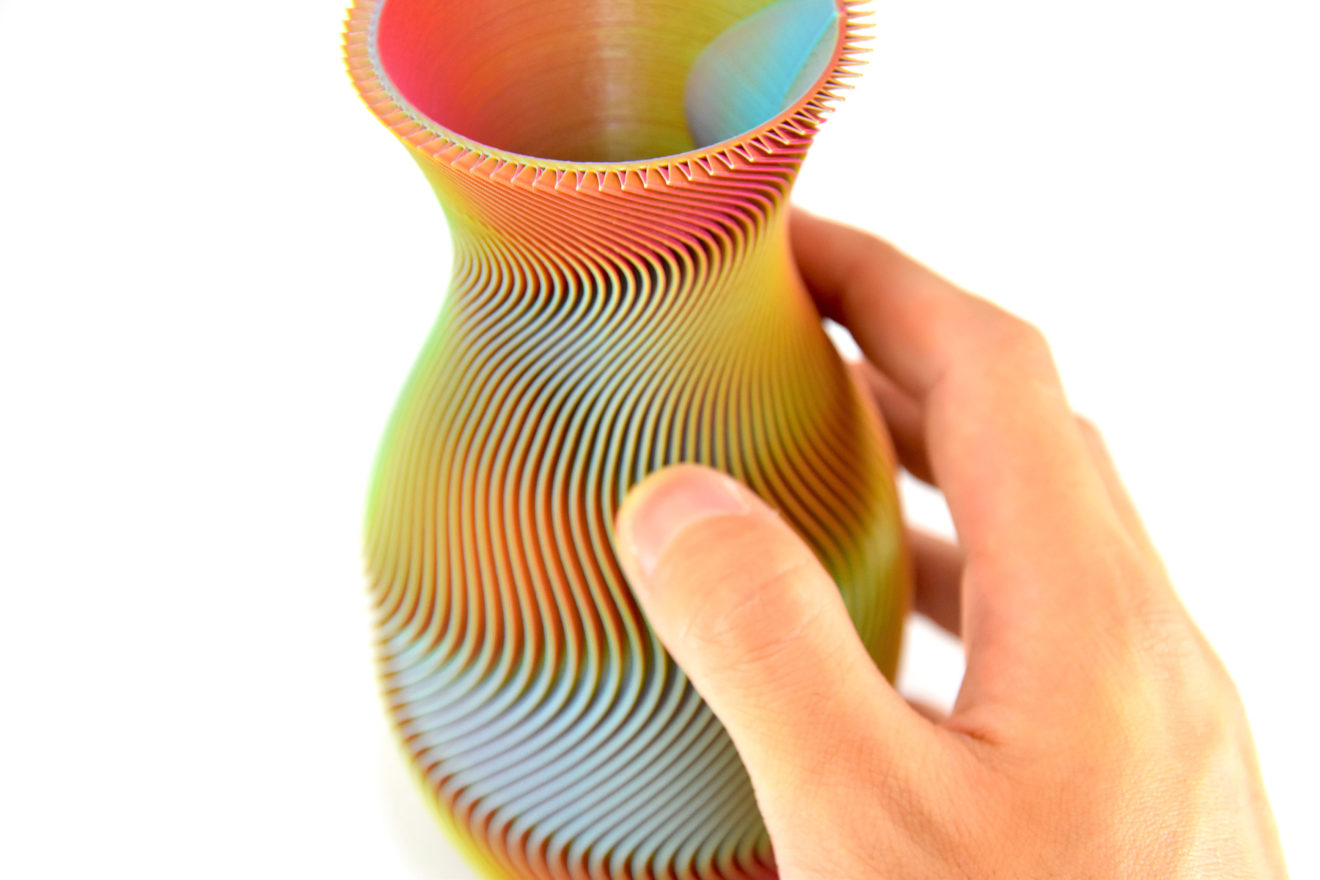
\includegraphics[width=12truecm]{./fig/sekisai.jpg}
  \caption{積彩によって印刷した造形物}
  \url{https://idarts.co.jp/3dp/toyamadesign-gp-color-fab/} % Web上のデータの場合、参照先URLを明記
  \label{fig:ferret}
\end{figure}

\section{放電現象を利用したインクジェット型金属3Dプリンター開発に関する基礎研究\cite{j}}
\label{sec:enum}
この研究では,熱可塑性樹脂を用いた材料押出型の3Dプリンターの機構をベースとした金属3Dプリンターの開発をしている.
従来の金属材料を扱うことのできる3Dプリンターの例として,積層造形,粉末床溶接接合,結合剤噴射,溶接肉盛などを利用したものがあるが,これらの方法は装置も大型で価格も非常に高い.
また,金属粉末の結合力が十分ではない指摘もされている.材料押出型で金属を扱える3Dプリンターが開発されれば,低価格な金属3Dプリンターが実現できる.

下に3Dプリンターの概略図を示す.この3Dプリンターには①細線繰り出し電極,②薄肉パイプ回転電極の二つの特徴がある.

\begin{figure}[H]
  \centering
  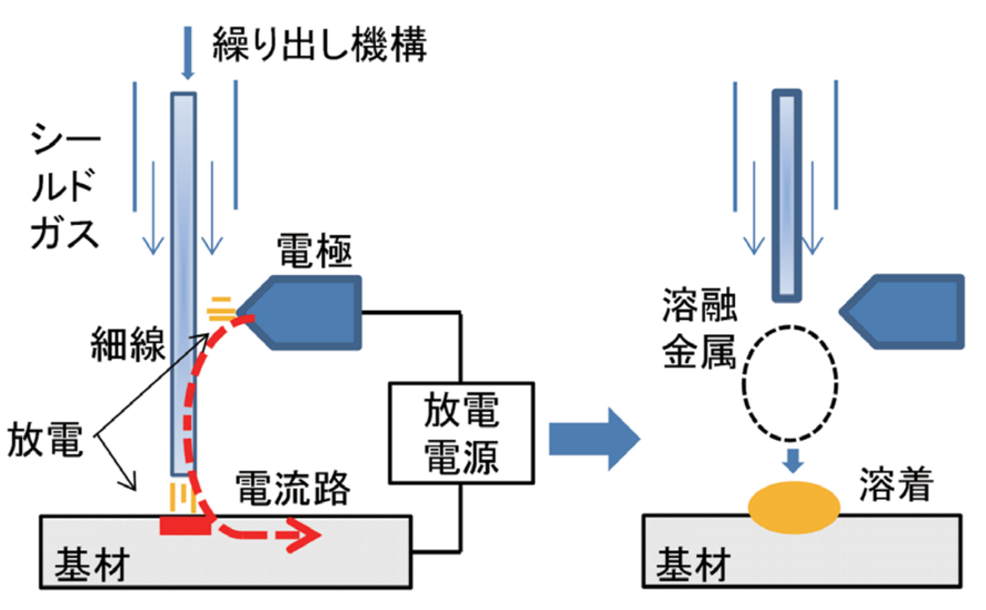
\includegraphics[width=10truecm]{./fig/houdenn.png}
  \caption{インクジェット型金属3Dプリンターの概略図}
  %\url{https://idarts.co.jp/3dp/toyamadesign-gp-color-fab/} % Web上のデータの場合、参照先URLを明記
  \label{fig:ferret}
\end{figure}



\section{高速・高精細金属3Dプリンターの開発\cite{k}}
\label{sec:enum}
この研究では,レーザーメタルでポジションという方法を採用した3Dプリンターの開発を行っている.
この方法はDEDとも呼ばれていて,レーザー粉末を同時に構造物へ照射し,粉末を溶かしながら造形を進める手法であるである以下に印刷している様子の模式図を示す.
レーザーをベースプレートに照射すると融解プールが形成される.金属粉末は,ノズルからキャリアガスとともに噴射され,形成された融解収束される.
供給された粉末は,プールで溶融し,これを冷却することで凝固する.

\begin{figure}[H]
  \centering
  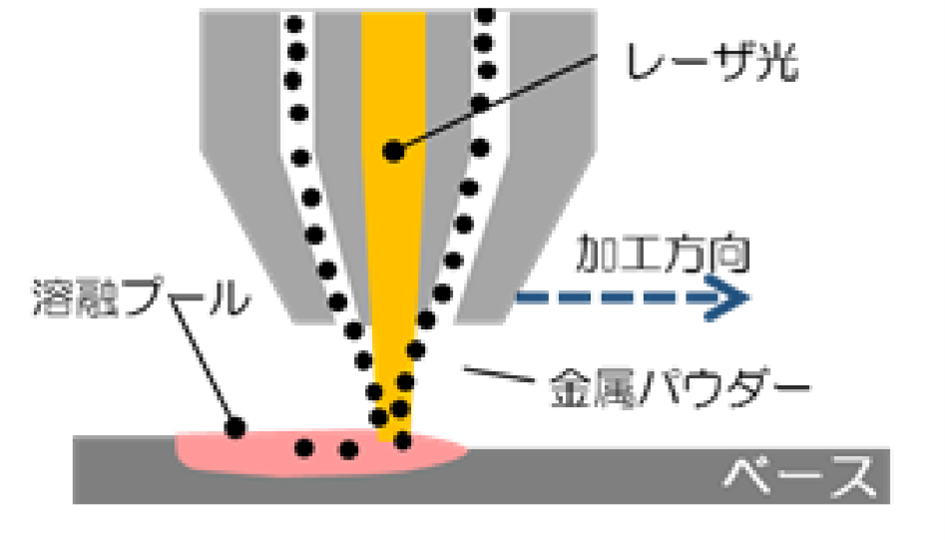
\includegraphics[width=9truecm]{./fig/kinnzoku.png}
  \caption{DEDの模式図}
  %\url{https://idarts.co.jp/3dp/toyamadesign-gp-color-fab/} % Web上のデータの場合、参照先URLを明記
  \label{fig:ferret}
\end{figure}

従来の金属3Dプリンターの多くは,パウダー・ベッド・フュージョン(PB)方式を採用している.
この方式では,パウダーベッドを作製し,造形部のみにレーザーを照射し溶融・凝固スキージとレーザー照射を繰り返して造形を進める.
しかし,高速造形のために高出力レーザーを用いると,パウダーのスパッターが多く発生してしまうという課題がある.
これにたいしDEDは,1.高出力レーザーが使用できるため造形速度が速い,2.局所パージを使用することで筐体レス化が可能となり,大型造形にも対応可能,3.複層造形が可能,などの利点がある.

また,いかにDEDを用いて作製した造形物を示す.
レーザー出力と粉末供給量を増加させることで造形速度が向上し,レーザー出力4kwのときに,最大で359cc/hの造形速度を実現した.

\begin{figure}[H]
  \centering
  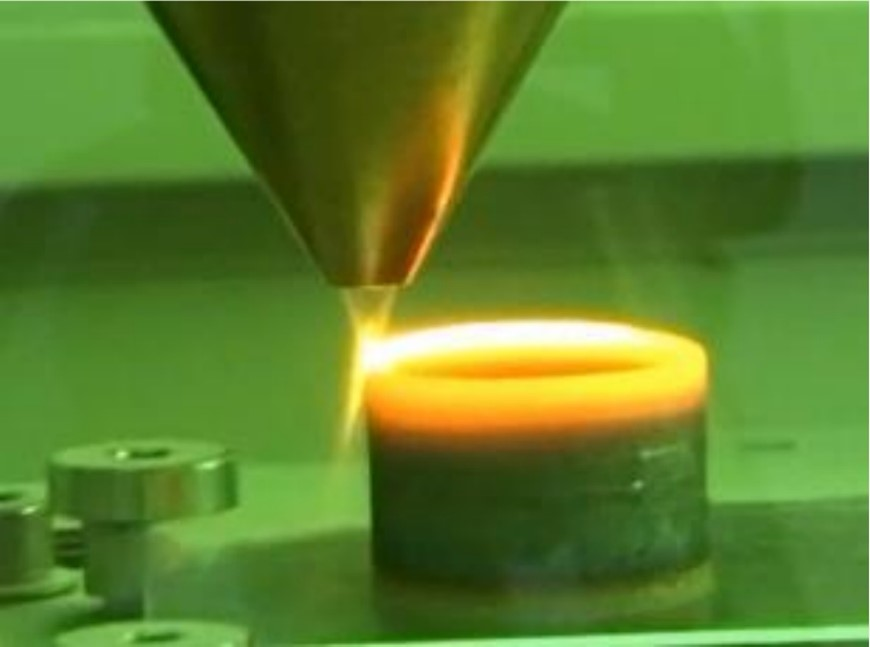
\includegraphics[width=11truecm]{./fig/kinnzoku2.jpg}
  \caption{DEDを用いて作製した造形物}
  %\url{https://idarts.co.jp/3dp/toyamadesign-gp-color-fab/} % Web上のデータの場合、参照先URLを明記
  \label{fig:ferret}
\end{figure}



\section{Robot-Assisted Rapid Prototyping for Ice Structures\cite{ss}}
\label{sec:enum}
この研究では,冷やした水を一滴ずつ垂らしながら氷をFDM の様に積み上げて造形する.
造形のスピードはかなり遅く 20mm/h で造形するが,精密な造形が可能で塩水をサポート剤として使用し,オーバーハングのある造形も可能になっている.
塩水でできた氷は水でできた氷よりも低い温度で溶け始めるため.0℃ の部屋で放置すれば塩水のラフトが溶け水の造形物だけが残る仕組みになっている.
この研究は精度を出すためにスピードを犠牲にしており普通のマグカップのサイズでも印刷に 50 時間近くかかる.
そのため,造形中に溶けないように冷凍庫の中のような環境の部屋で造形する必要がある.


\begin{figure}[H]
  \centering
  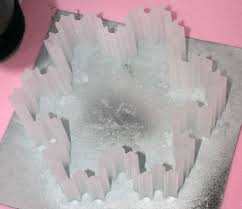
\includegraphics[width=9truecm]{./fig/Robo.png}
  \caption{塩水を使ったラフト}
  %\url{https://idarts.co.jp/3dp/toyamadesign-gp-color-fab/} % Web上のデータの場合、参照先URLを明記
  \label{fig:ferret}
\end{figure}


\section{Elsa:氷を素材とした3d プリンターの開発\cite{h}}
\label{sec:enum}
この研究は造形速度と造形精度を両立させ,一般に普及している3Dプリンターを同じ学習コストで使える氷をマテリアルとした 3D プリンターの開発を行っている.
1つ目の手法として液化した代替フロン (HFC134a) を使用する方法を提案している.
フロンが断熱膨張する際に周囲の熱を奪うのを利用して水を冷やし,瞬時に氷を作る.エアーブラシを使い水とフロンガスを噴射し氷を作る機構を実装した.
しかし,3つの問題点がある.1つ目は,コストが高いことである.3つ目は,造形物がフロンガスを含み純粋な氷ではないこと.3つ目は,環境に対して悪影響があることである.

\begin{figure}[H]
  \centering
  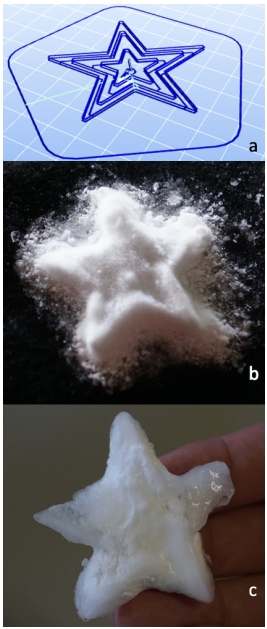
\includegraphics[width=6truecm]{./fig/erusa1.jpg}
  \caption{フロンガスを用いて作製した造形物}
  %\url{https://thelastnewspaper.com/a-layered-fabric-3d-printer-for-soft-interactive-objects/} % Web上のデータの場合、参照先URLを明記
  \label{fig:ferret}
\end{figure}

2つ目の手法として液化した代替フロン (HFC134a) を使用する方法の問題を解決できる氷をマテリアルとした3Dプリンターとして、液体窒素を使用する手法を提案している.

\begin{figure}[H]
  \centering
  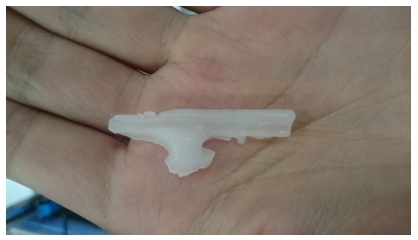
\includegraphics[width=10truecm]{./fig/erusa2.jpg}
  \caption{液体窒素を用いて印刷した造形物}
  %\url{https://thelastnewspaper.com/a-layered-fabric-3d-printer-for-soft-interactive-objects/} % Web上のデータの場合、参照先URLを明記
  \label{fig:ferret}
\end{figure}

\section{関連研究のまとめ}
\label{sec:enum}

本研究では従来にはない,新たなマテリアルを使った造形をするため,プラスチックではないマテリアルを使い造形物を印刷している研究を多く調べた。
関連研究の多くは,常温で安定している物質であり,加工が容易なものや温度変化によって性質が変わるものがマテリアルとして最適なものであることが分かった.
また,3Dプリンターに関して,近年新たなマテリアルの研究が数多く行われているのと同時に,新しい造形方法の研究が進められていることが分かった.
静電インクジェット式3Dプリンタによる高粘度食品材料の高精度プリント\cite{e}などでは,静電気を使い,超微細な造形を行おうことが出きる.水も僅かに電荷をい帯びているため,この方法を利用して超微細な氷の造形などもできるのではないかと考えた.
このように,新しい造形方法が開発されると,これまで造形に適してないと思われていたマテリアルも造形への可能性が生まれるため,新た造形方法を調査の必要性がある.

マテリアルが,プラスチックであるが積彩\cite{h}の美しさと造形方法は氷をマテリアルとした造形と通じるものがある.
美しさでは,氷をマテリアルとした造形では,溶け出すことで,一度として同じ瞬間が無く,その変化を楽しむという特徴がある.
積彩,でも造形物の見る角度を変えると色が変化し,七色のように見える.
このように同じ瞬間が無く,変化し続けて見えるもに美しさを感じる部分があるので考える.
造形方法についても,複数の色のフィラメントをノズル内で混ぜ,押し出し造形強いる.
この技術を発展させれば,Robot-Assisted Rapid Prototyping for Ice Structures \cite{ss}のような塩水と水の使い分けが1つのノズルできるのではと考える.
このような既存の技術の発展についても新たなマテリアルでの造形を行う際の参考になった.

本研究は,一般の人でも扱いが可能かつ,一般の3Dプリンターと同程度の速度とある程度の精度を両立した氷をマテリアルとした3Dプリンターとして,
造形精度としてはElsa:氷を素材とした3d プリンターの開発 \cite{h} とRobot-Assisted Rapid Prototyping for Ice Structures \cite{ss} の中間のプリンターを目指し,
一般の人でも扱いが可能なプリンターを開発した.

	
\chapter{仮説と提案}
\label{chp:first}

\section{氷をマテリアルとした3Dプリンター}
\label{sec:paragraph}

3Dプリンターに実装した,氷を作るための機構について述べる.
これまでの氷の造形方法は大きく分けて2つある.大きな氷から切削して造形するもの.
もう一つが,水を少しずつたらし長時間をかけて,造形するのもがある.
どちらも取り扱いが難しく,造形するのに長時間を要してしまうのが問題だ.
また,短時間できる氷の造形として,過冷却水を使っての造形が有名である.
しかし,過冷却水の場合準備に時間がかかる上,温度変化に敏感で少しの衝撃でも凍り始めてしまうため,制御が難しい.
一般の人でも扱いが可能かつ,一般のユーザーが設計したデータにできるだけ近い形に印刷できる氷をマテリアルとした3Dプリンターの提案する.
必要な要素としては以下のようである.

\begin{enumerate}
  \item ある程度の精度で造形ができること. 
  \item 通常の3Dプリンターと同程度の速度で印刷ができること.
  \item 氷の定義を満たしていること.
  \item 3Dプリンターが扱える人であれば,短時間で扱えるようになること.
 \end{enumerate}

それぞれの要素について実装にするにあたり、以上のことが有効ではないかと考える.
「ある程度の精度で造形ができること.」「通常の3Dプリンターと同程度の速度で印刷ができること.」を満たすために液体窒素を使った造形方法が有効ではないかと考える.
また,他の研究では,特殊な機材を使用し,装置が高価になりがちである.液体窒素は,日本各地で手に入る上,価格も1リットルあたり300円と安価であるため,今回の研究で使用することにした.
「3Dプリンターが扱える人であれば,短時間で扱えるようになること.」を満たすためには,既存の3Dプリンターと同様の使用方法で使える必要があるため,世界中で使用されている3Dプリントおよびスライサーソフトウェアである Ultimaker Cura で操作が可能である必要があると考える.
氷の定義をしたことで、純粋な水以外でも氷の造形ができる.純粋な水を積層する場合,水の粘度が低いため,固まる前に広がってしまう.そのため造形精度が悪く,造形物のからはみ出した部分には造形ができず,オーバーハングなども造形することが難しい.
よって,水の粘度を上げることにより,上記の問題を解決できるのではと考える.また,粘度を上げる手段として,いくつかの方法が考えられる.
水に砂糖などを加え粘度を上げる方法とシャーベット状のものをマテリアルとして使用する方法だ.シャーベット状のものを使用する場合は,温度管理が必要になるため,今回の機構では,砂糖を加え粘度を高めたものをマテリアルとして使用する.


\chapter{機構の実装}
\label{chp:first}

\section{予備実験}
\label{sec:paragraph}

水に砂糖等の粘度を上げられる物質を添加し造形を行う方式の実証を行った.
初めに,3D プリンターとして自動化させる前に,水の粘度が造形物の造形速度,造形精度,オーバーハングの造形に影響を与えるのか調査を行った. 
造形の仕組みは図のようになっている.実験の装置は, 保温のため一番下に発泡スチロールの容器を用意した.
その上に-196 度の液体窒素を十分に注ぎ,さらにその上からアルミトレーを沈める.
それにより,アルミトレーも液体窒素に近い温度まで冷やされ,そこに注射器を使い水あめと水の中間の粘度の水をたらすことで,冷やされた水が氷に変わる.
冷やされた氷の温度は 0 度よりも低く,その上に水をたらすと氷柱ができるように氷が積層される. 

\begin{figure}[H]
  \centering
  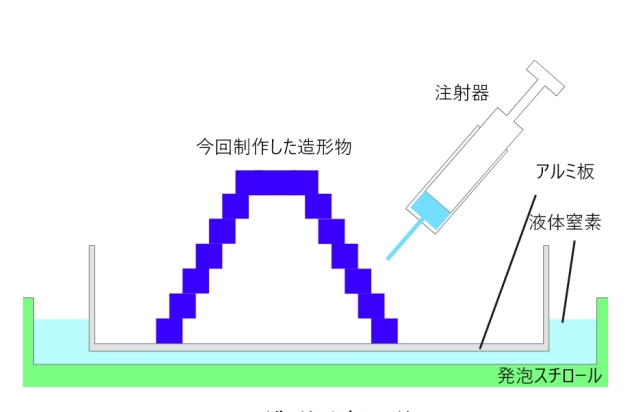
\includegraphics[width=10truecm]{./fig/yobi2.jpg}
  \caption{設計図と造形した形}
% \url{http://www.this.is.sample.url/} % Web上のデータの場合、参照先URLを明記
  \label{fig:yobitamesi}
\end{figure}

\begin{figure}[H]
  \centering
  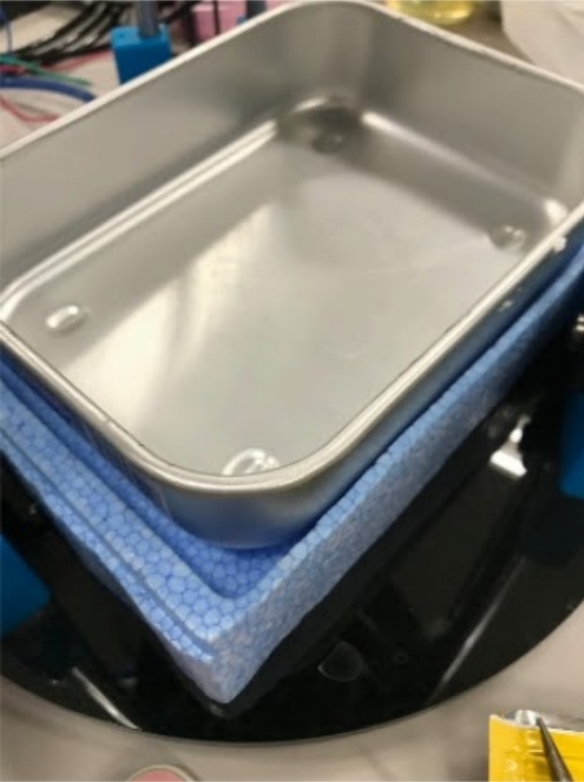
\includegraphics[width=10truecm]{./fig/yobi34.jpg}
  \caption{制作した実際の装置}
% \url{http://www.this.is.sample.url/} % Web上のデータの場合、参照先URLを明記
  \label{fig:yobipure}
\end{figure}

制作した装置は図4.1である.この装置を使い,水の粘度がどの程度、造形速度と造形精度に影響するのか調査を行った.
造形物はオーバーハングの調査を行うため図のように中を空洞になるように造形を行った. 実際に制作した装置を使い造形を行ったものが図である.
造形時間は約 5 分ほどで完成した.造形精度の問題もあるが通常の3Dプリンターよりもかなり早い結果になった.
大きさは横幅約 3 センチ,高さ約 1.5 センチほどである.使用した水の量は,約 200ml ほどである.
初めに想定した形通りに造形ができ,オーバーハングの造形も成功した.また,発見した特徴として,透明度の高い氷を制作することができた.

\begin{figure}[H]
  \centering
  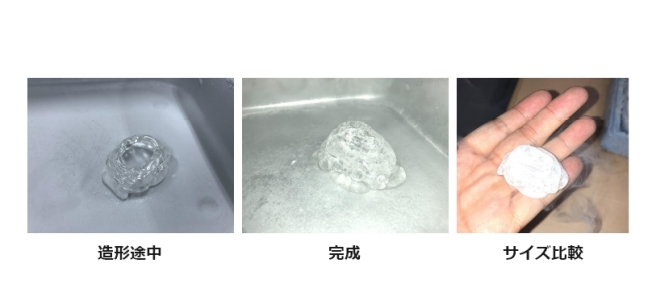
\includegraphics[width=14truecm]{./fig/yobi.jpg}
  \caption{造形過程と完成物}
% \url{http://www.this.is.sample.url/} % Web上のデータの場合、参照先URLを明記
  \label{fig:yobikekka}
\end{figure}

結果は予想通り,造形速度の改善と、オーバーハングができない問題の解消,これら二つを改善しつつ,さらに造形精度の向上ができた.
通常のプラスチックをプリントする 3D プリンターと比較して,押し出される水の粘度が関係していることが分かった.
また,造形する際に使用した水が砂糖を溶かすために加熱していたた.この余熱があったため,注射器から押し出すときの温度が 50 度くらいになっていた.
そのため,液体窒素の注射器内部の水が冷え固まらず,すでに造形されている造形部分の表面を溶かすため,造形物が水をはじくことなく接着できているのではないかという仮説が仮説を立てることができた.



\section{造形の仕組み}
\label{sec:paragraph}
予備実験では,液体窒素と水に砂糖を混ぜ粘度を上げることにより,ある程度の精度と速度を持つ事が分かった.
ここでは,予備実験を自動化させ,プリンターが氷を積層造形していく仕組みについて解説する.
造形用のペットに熱伝導率の高い金属製のアルミプレートを使用し、液体窒素の保温性を高める為発泡スチロールでできた容器に沈めた.
液体窒素は-196℃であり,アルミプレートもそれに近い温度まで冷やされる.そこに水をたらすことで,水が冷やされ氷が作られる.
氷は,アルミプレートを通して、液体窒素により冷やされ続けるため,氷の温度も0℃以下になる,その上に水をたらすとその水も氷へと状態が変化し氷が積層される.


\begin{figure}[H]
  \centering
  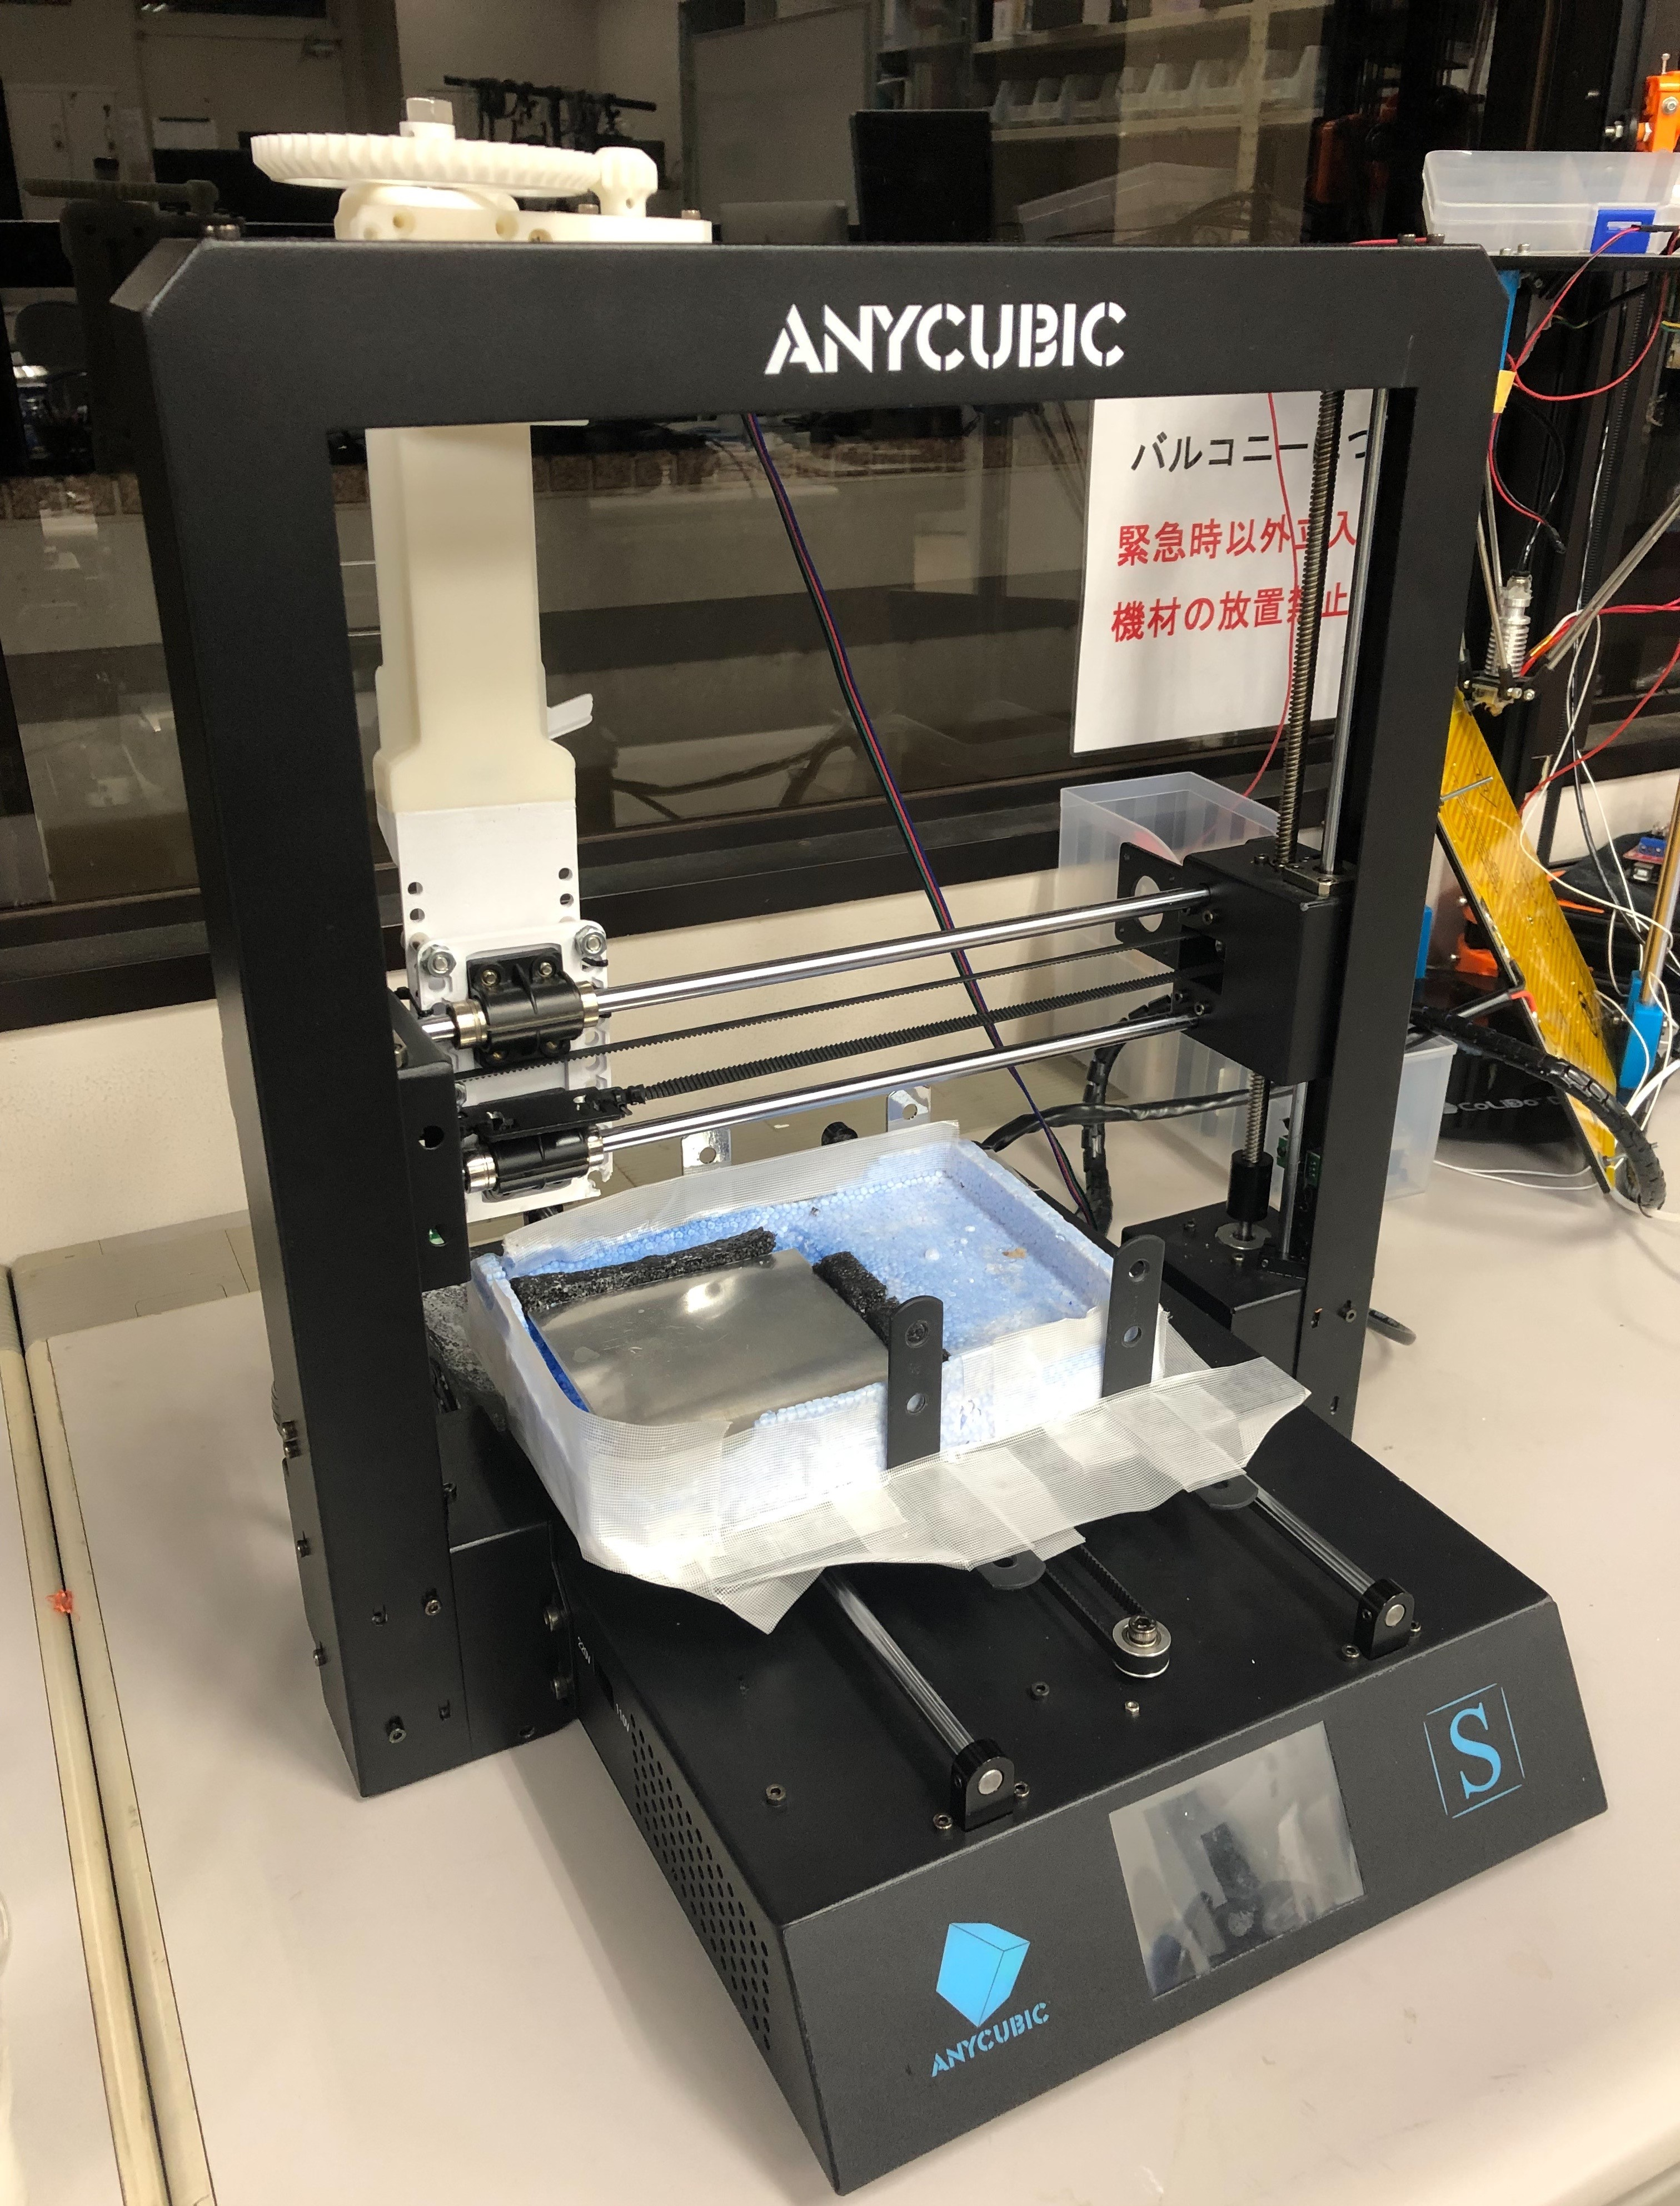
\includegraphics[width=7truecm]{./fig/printer.jpg}
  \caption{開発した氷をマテリアルとしたプリンターの全体図(前)}
% \url{http://www.this.is.sample.url/} % Web上のデータの場合、参照先URLを明記
  \label{fig:printer}
\end{figure}


\begin{figure}[H]
  \centering
  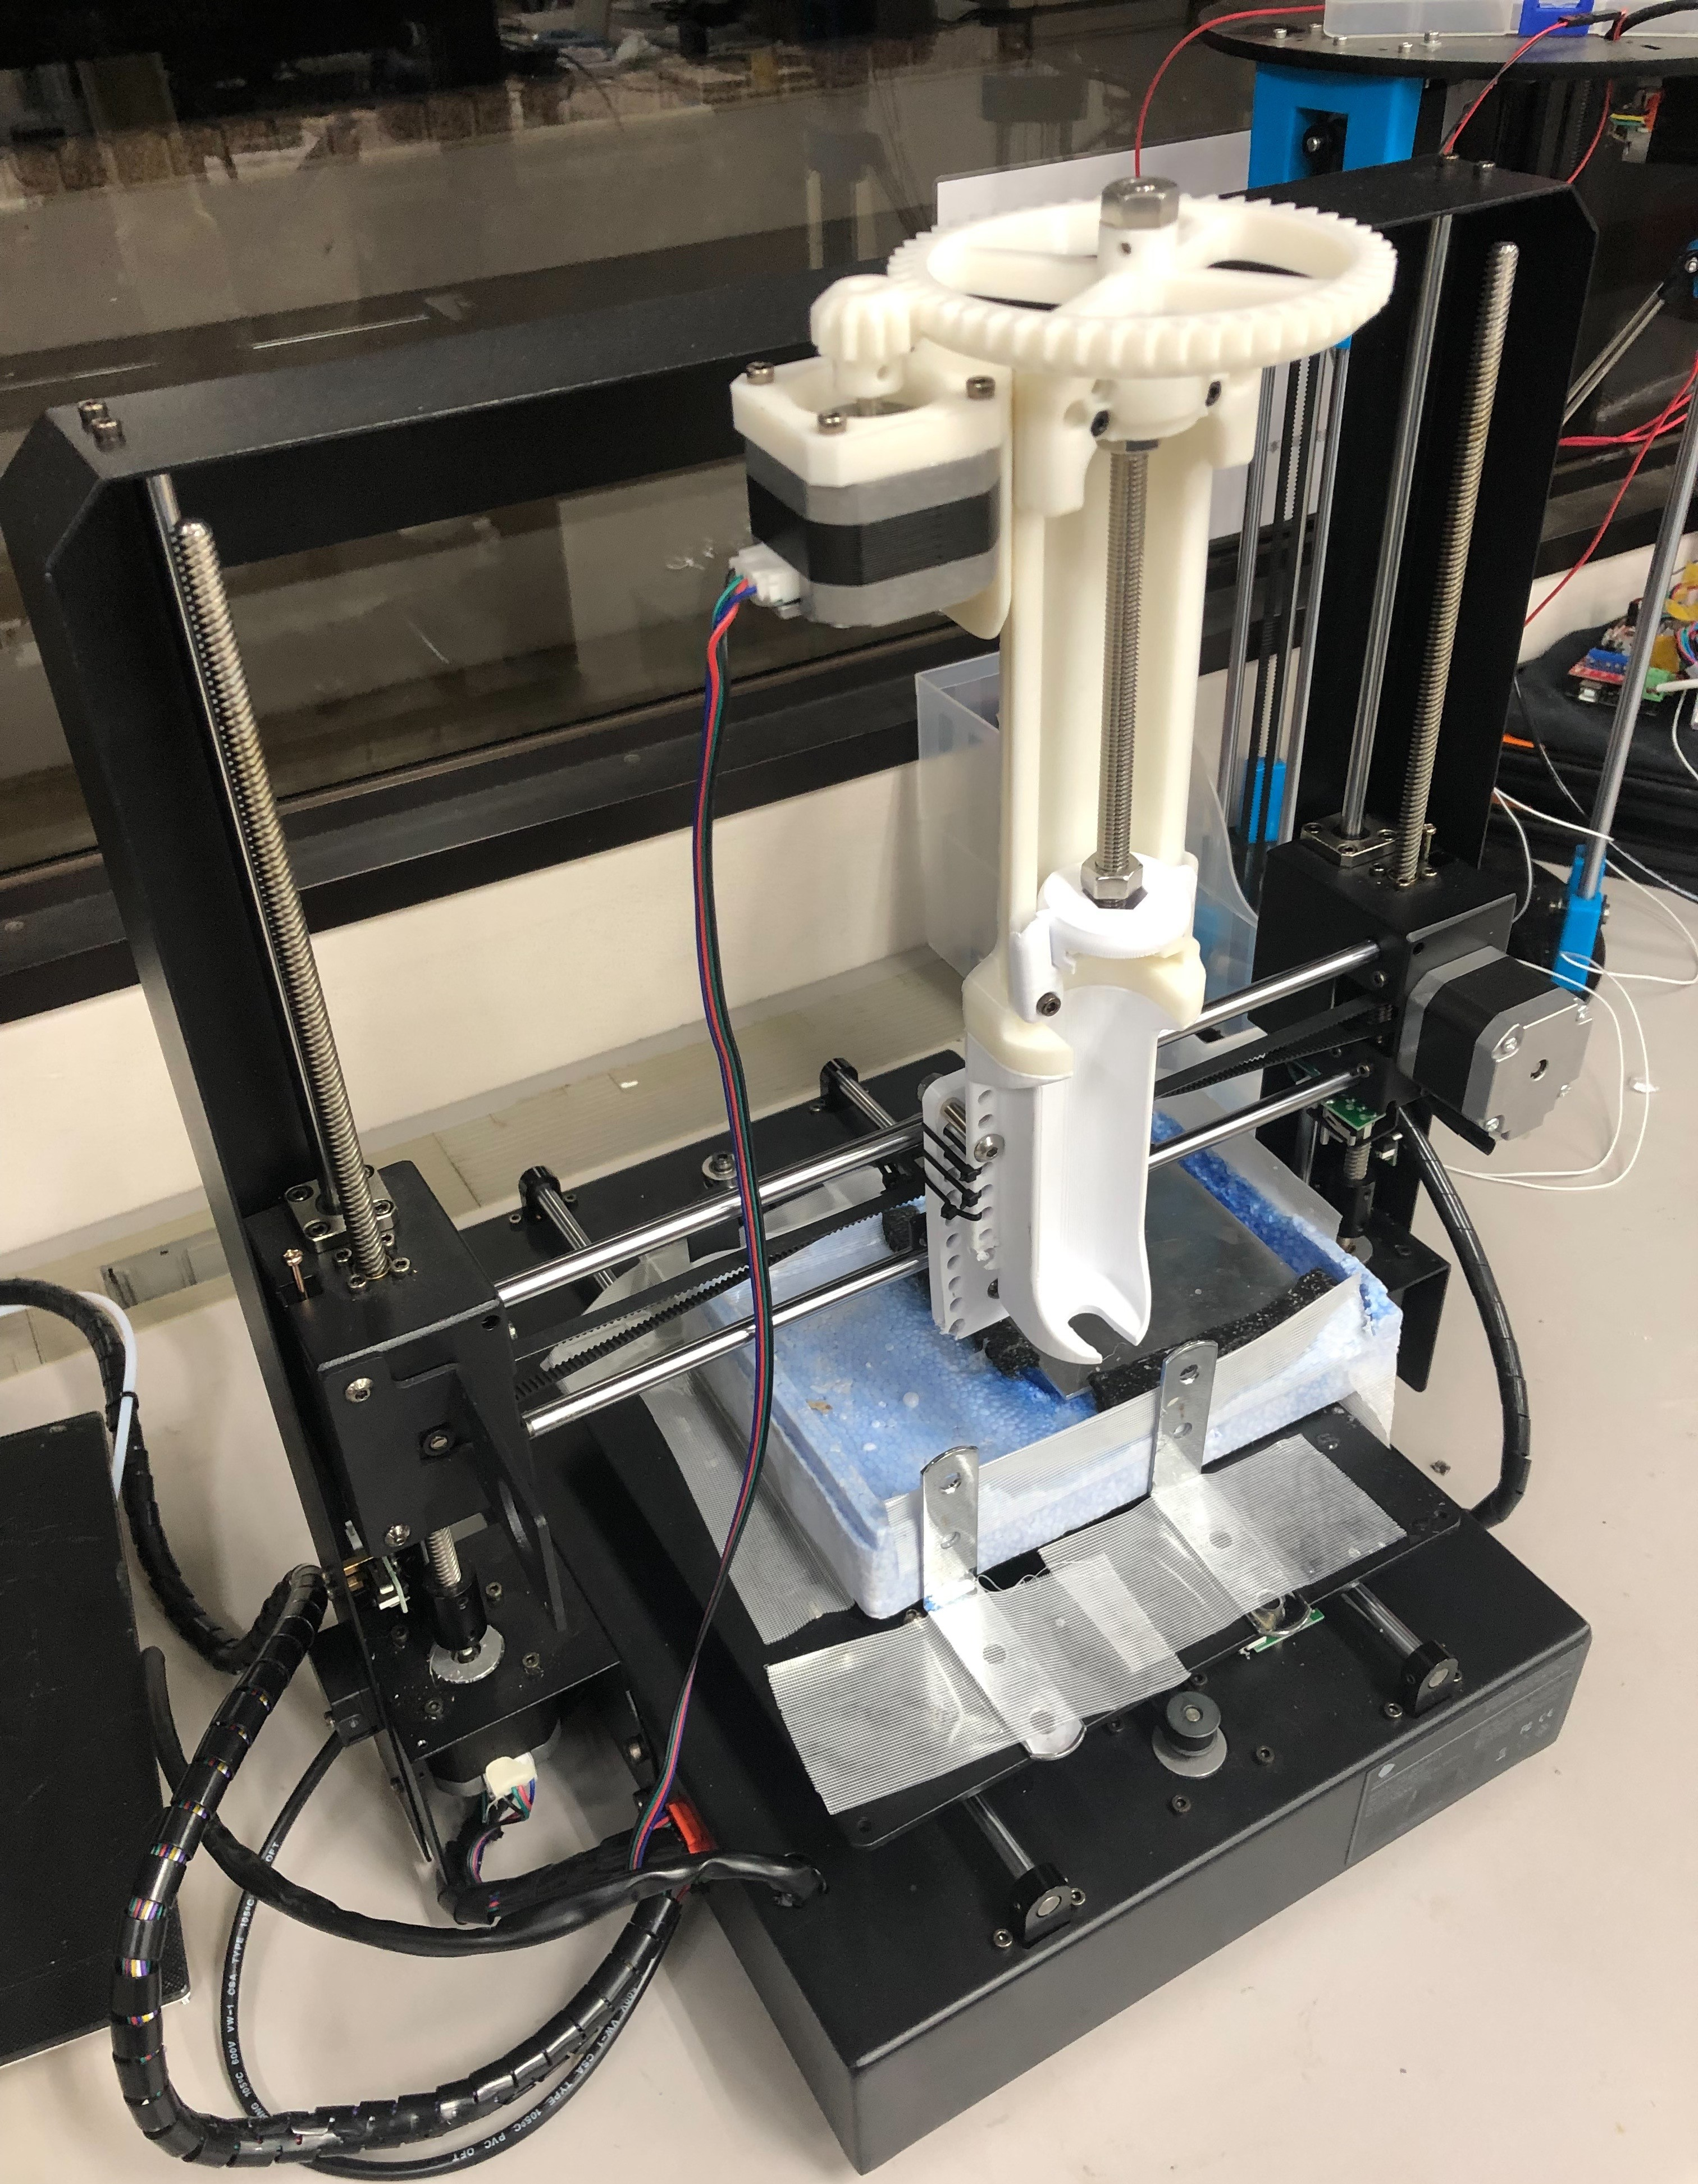
\includegraphics[width=7truecm]{./fig/printer2.jpg}
  \caption{開発した氷をマテリアルとしたプリンターの全体図(後)}
% \url{http://www.this.is.sample.url/} % Web上のデータの場合、参照先URLを明記
  \label{fig:printer2}
\end{figure}



\section{液体窒素を用いた造形の実装}
\label{sec:paragraph}
ここでは,液体窒素を使用した造形機構について述べる.
機構の全体像は図のようになっている.
ノズルから水を供給するためのシリンジを押し出す機構を実装した.
また,今回の水は粘度を持たせているため,長いチューブを用いてしまうと,抵抗で押し出すのが難しくなる.そのためシリンジからノズルまでの距離ができるだけ短くなる機構を実装した.

\section{プリンターの本体}
\label{sec:paragraph}
3Dプリンターも一般に販売されているものを改造して使用した.使用した3Dプリンターは,「 Anycubic i3 Mega S 」である
一般に売れれている3Dプリンターの改造で氷をマテリアルとした造形ができれば,3Dプリンターが使える一般の人が短期間に学習が可能だと考える為である.
また、大半が既存の部品であるため,一般への普及もしやすいと考えるためである.

\section{プリンターの制御}
\label{sec:paragraph}
氷の3Dプリンターの制御は,Marlin-Ai3Mという3Dプリンターの制御用アプリケーションとMarilnというファームウェアを一部改造し使用している.
改造内容は,モーターの駆動方向の変更,モータードライバーへの対応,3Dプリンターは安全装置として,一定の温度以下で作動しないようになっている.
この安全装置が0℃以下で稼働する氷の3Dプリンターでは必要が無いため,無効にさせた.
今回制作したプログラムは,Ultimaker Curaを通して「 Anycubic i3 Mega S 」にアップロードさせた.
この作業を行ったことにより,基本的に一般に販売されている3Dプリンターと同じように制御することができる.

\section{シリンジの機構}
\label{sec:paragraph}
シリンジを押し出して水を供給するために,既存のエクストルーダー用のモーターを利用している.
シリンジを押し出すためにモーターの回転を上下の運動へ置き換えるために、全ねじ棒を使用した.また,そのままモーターを直結してしまうと,力不足になることが想定されてため,ギヤで回転数を調整している.
既存の3Dプリンターでは、フィラメントを押し出すモーターを利用しているため,PCを使い水の押し出し量を自由に調整することが可能であり,安定して造形ができる設定を模索することができる.
また,シリンジは3Dプリンターを使い制作したが,サイズが研究室にあるプリンターに収まりきらなかったため,上下に分割して印刷し,印刷後接着剤により合体させている.

\begin{figure}[H]
  \centering
  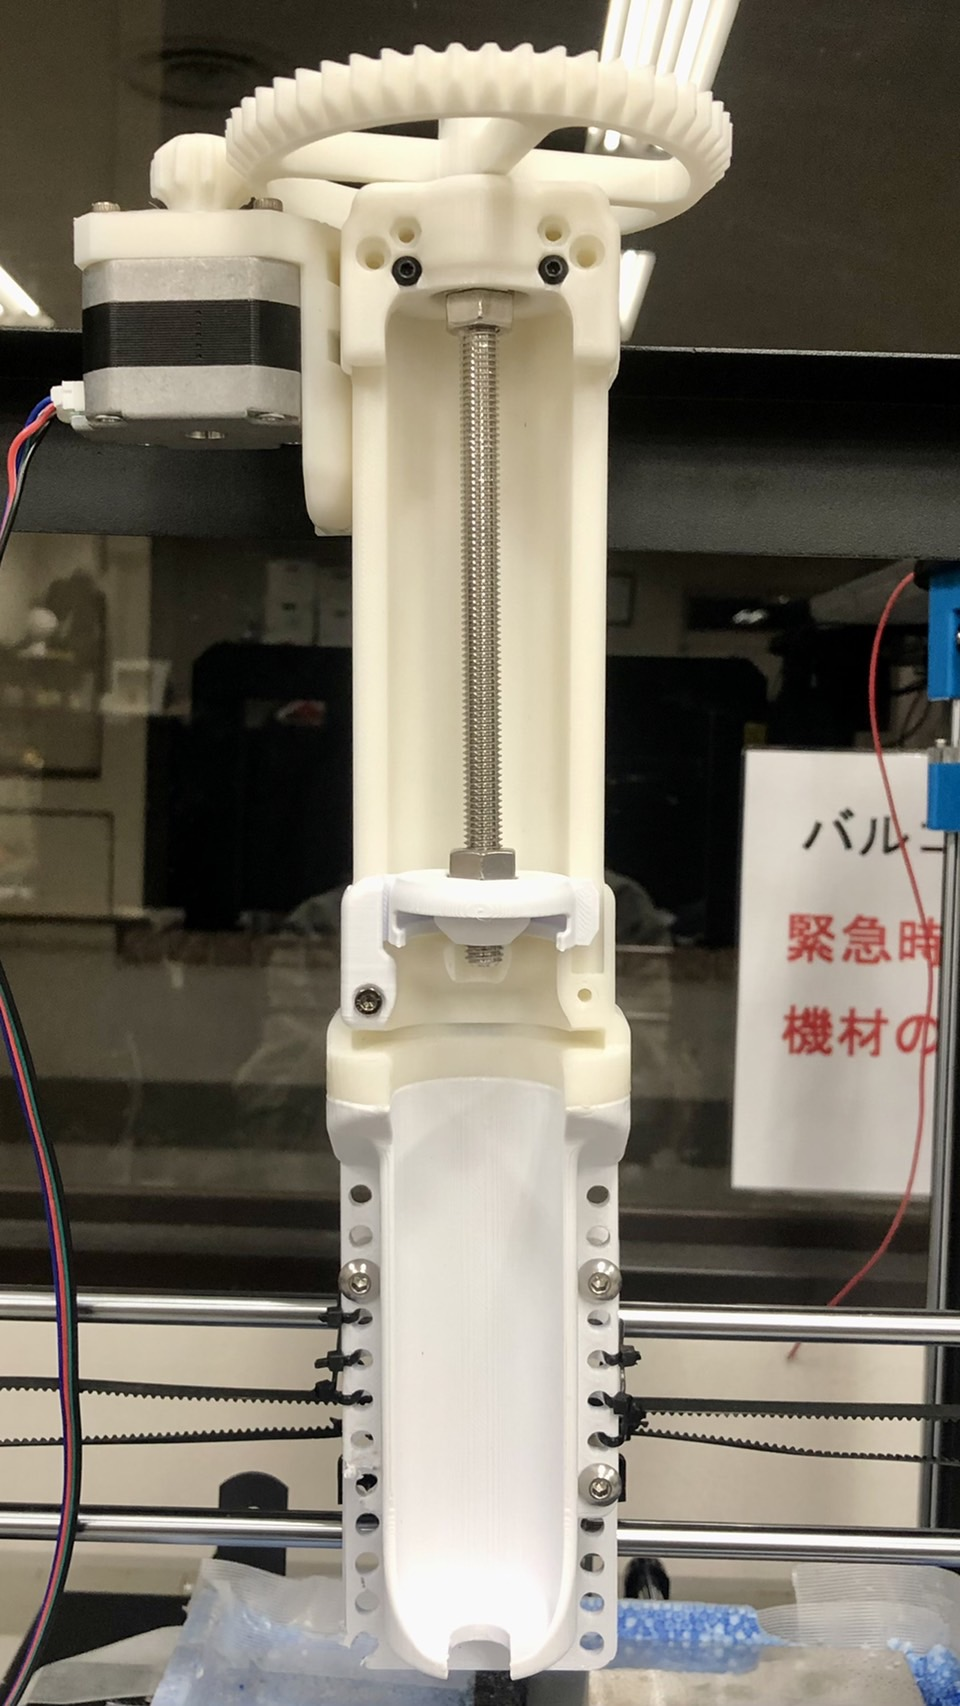
\includegraphics[width=7truecm]{./fig/101285897.jpg}
  \caption{シリンジの機構}
% \url{http://www.this.is.sample.url/} % Web上のデータの場合、参照先URLを明記
  \label{fig:printer2}
\end{figure}

\section{ノズルの機構}
\label{sec:paragraph}
水に砂糖を加え,粘性を持たせた液体を流すため,シリンジからノズルまでの距離が長いとその間で抵抗が発生しシリンダーやシリンダー制御用のモーターに負担をかける.
そのため、できるだけ,シリンジからノズルの距離が近い方がいいと考える.
そこで,シリンジを直接ノズルとして使用し,素材を押し出せる機構を制作した.
また,ノズルサイズは今回の実験では1mmである.市販されているシリンダーの先をヒートガンで溶かし,先を塞いだ後にドリルによって穴を空けた.


\begin{figure}[H]
  \centering
  \includegraphics[width=13truecm]{./fig/sirinda.jpg}
  \caption{ノズル}
% \url{http://www.this.is.sample.url/} % Web上のデータの場合、参照先URLを明記
  \label{fig:stage}
\end{figure}

\section{ベッドの機構}
\label{sec:paragraph}
液体窒素で氷を造形するベッドとして、大きく2つに分けられる.1つ目が液体窒素用のトレーだ.液体窒素用のトレーでは,下に保温性を高め、液体窒素の持ち時間を長くするために、発泡スチロールを使用した.
また,アルミプレートの下に液体窒素がたまるようにくぼみをつけている.2つ目が造形用のトレーだ.熱伝導率の高い金属のプレートを使用する.今回はアルミ製のプレートを使用した.
また,造形したものを取り出しやすくするために、取り外しが容易な設計を行った.完成したハードは図4.8 のようになっている.

\begin{figure}[H]
  \centering
  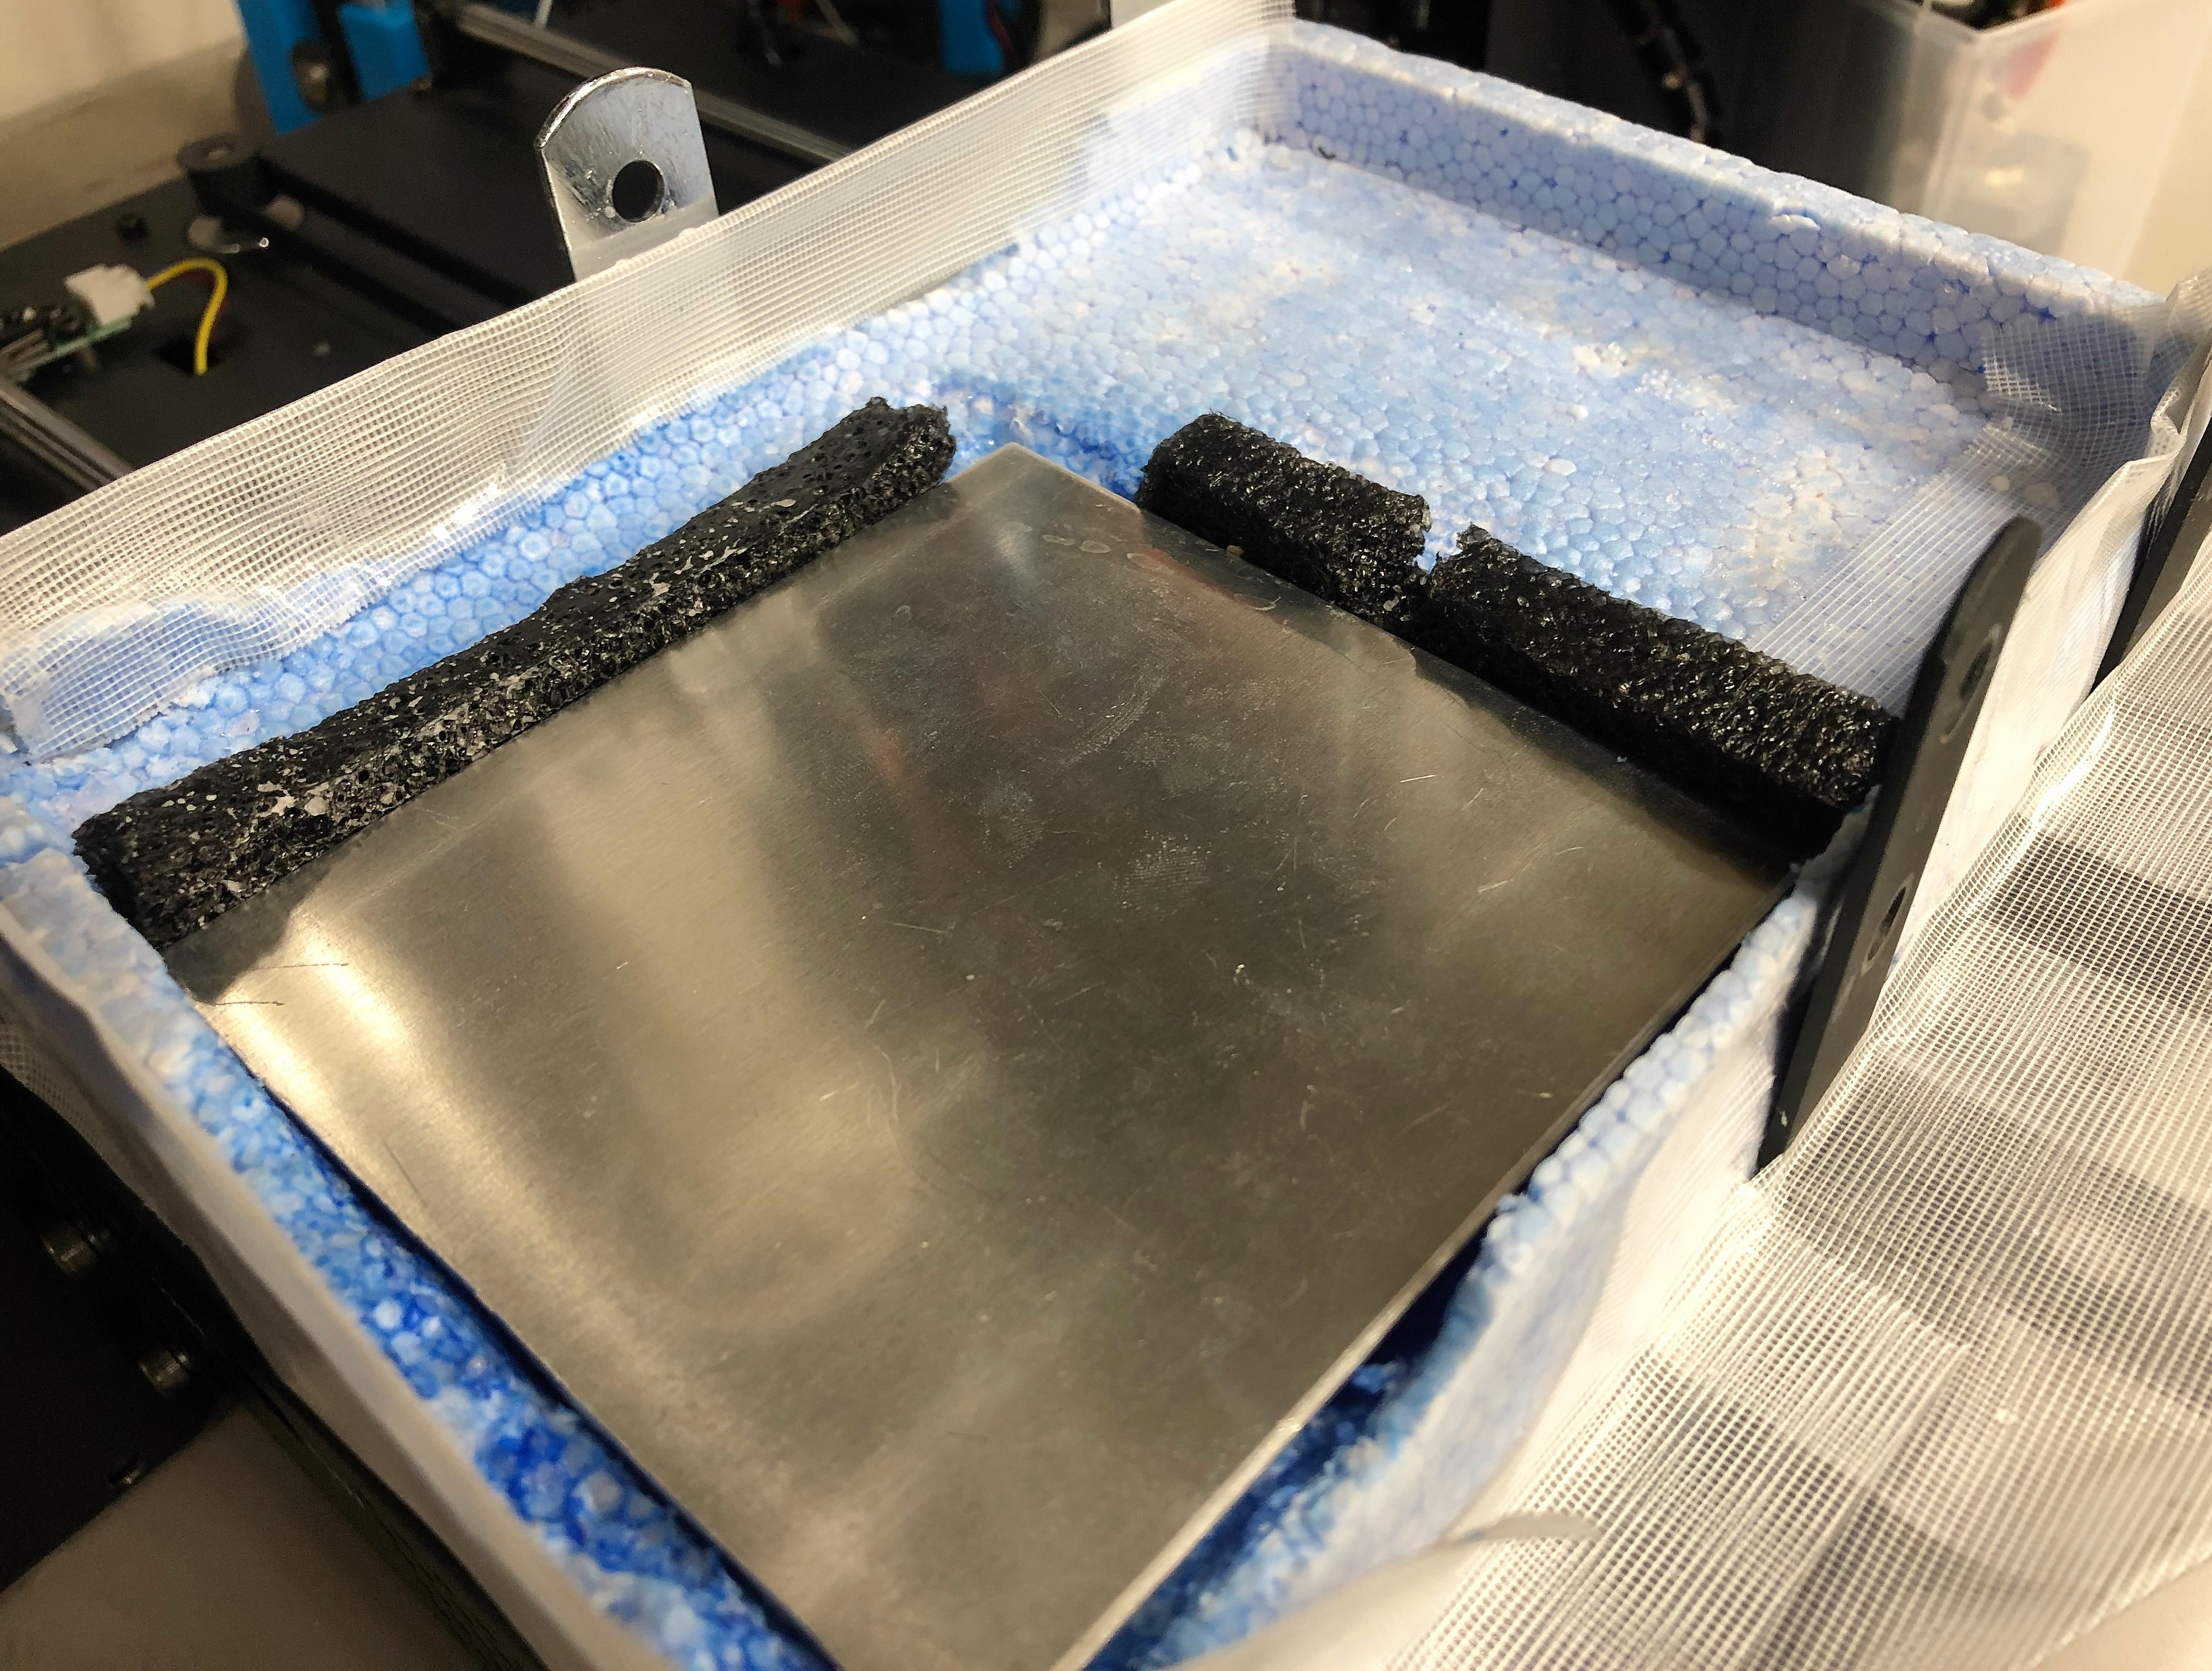
\includegraphics[width=9truecm]{./fig/stage.jpg}
  \caption{液体窒素造形用ベッド}
% \url{http://www.this.is.sample.url/} % Web上のデータの場合、参照先URLを明記
  \label{fig:stage}
\end{figure}

\section{マテリアルの検討}
\label{sec:paragraph}
今回開発する3DプリンターFDM方式の改良である.FDM方式では,常温で固体の物質を加熱し柔らかくしてから押し出している.
水のプリントの場合,既に液体を押し出し,冷やして固体にしてプリントする.
違いとして,押し出されるときのマテリアルの粘度が印刷精度や印刷時間に違いをもたらしているのではと考える.
今回開発した氷をマテリアルとして3Dプリンターの材料として水に砂糖を混ぜて粘度を上げたものを用意した.砂糖はどこでも手に入りかつ安価で扱いも簡単であるため,今回の実験に採用した,
水と砂糖の割合は 1:3 のものを用意した.
また, 1:3 の液体を作るにあたり,鍋で一度加熱する必要がある.

\begin{figure}[H]
  \centering
  \includegraphics[width=13truecm]{./fig/sugar.jpg}
  \caption{砂糖を添加した割合ごとの水}
% \url{http://www.this.is.sample.url/} % Web上のデータの場合、参照先URLを明記
  \label{fig:stage}
\end{figure}

		% 第1章
\chapter{実験}
\label{chp:first}

\section{プリンターの動作検証}
\label{sec:paragraph}



\section{ノズルの高さ,移動速度,水の量による造形の変化}
\label{sec:paragraph}

\section{動作の確認}
\label{sec:paragraph}


\section{動作の確認}
\label{sec:paragraph}

	
%\chapter{使用例}
\label{chp:first}

\section{段落と改行}
\label{sec:paragraph}


\chapter{今後の展望}
\label{chp:first}

\section{段落と改行}
\label{sec:paragraph}

段落頭の字下げは自動で行われるため、全角スペースによる手動調整は不要であり、禁止である。
\LaTeX ソース中での改行は空行を挟まない場合は無視される。
ソース内では自分で編集しやすいように改行してよい。

このように、空行を挟むと改段落となる。
また、強制改行は\\このように \verb+\\+ で強制的に行うことができる。
しかし、この場合は段落の字下げもされないため、改段落を行う用途には空行を用いるべきで、
強制改行(\verb+\\+)は利用すべきではない。

しかしながら、例えば \verb+\verb+ 環境やインライン数式を用いる場合などで、
\verb+abcdefghijklmnopqrstuvwxyzABCDEFGHIJKLMNOPQRSTUVWXYZ+ 
というようにページ幅を超えてしまったり、前の行が間延びしてしまうようなケースがある。
そのような場合、\verb+\\+ を用いて強制改行により \\
\verb+abcdefghijklmnopqrstuvwxyzABCDEFGHIJKLMNOPQRSTUVWXYZ+ 
というように用いるとよい。

\section{箇条書き}
\label{sec:enum}

数字を使った場合の箇条書きの例を示す。

\begin{enumerate}
 \item 数字の付いた箇条書きの例
 \item こんな感じで手順などを列挙
\end{enumerate}

数字を付けずに列挙したい場合は itemize 環境を使う。
このようにあるキーワードを指定して \verb+\begin(}+ と \verb+\end{}+ で
囲む範囲のことを○○環境と呼ぶ。

\begin{itemize}
 \item 順番などを伴わない箇条書きの例
 \item 材料や要素を純粋に列挙したい場合に使用
\end{itemize}

enumerate 環境や itemize 環境は、入れ子構造を持つことができる。
例えば enumerate 環境の場合、以下のようになる。
\begin{enumerate}
 \item 東京都
 \begin{enumerate}
  \item 八王子市
  \item 多摩市
 \end{enumerate}
 \item 神奈川県
 \begin{enumerate}
  \item 横浜市
  \item 川崎市
 \end{enumerate}
 \item 山梨県
\end{enumerate}

\section{図表と参照}
\label{sec:fig_tbl}

図を挿入する際は以下のように書く。
必ずキャプションを付けるとともに、図に対する説明を本文中で記載すること。
何かの手違いで図が表示されなくなったとしても、文章で意味が通じるくらいに説明するのを目安にすること。
以下の図 \ref{fig:sample} と図 \ref{fig:ferret} は、適当なサンプル画像である。

\begin{figure}[H]
  \centering
  
\includegraphics[width=6.4cm]{./fig/fig-sample.eps}
  \caption{適当なサンプル}
% \url{http://www.this.is.sample.url/} % Web上のデータの場合、参照先URLを明記
  \label{fig:sample}
\end{figure}

\begin{figure}[H]
  \centering
  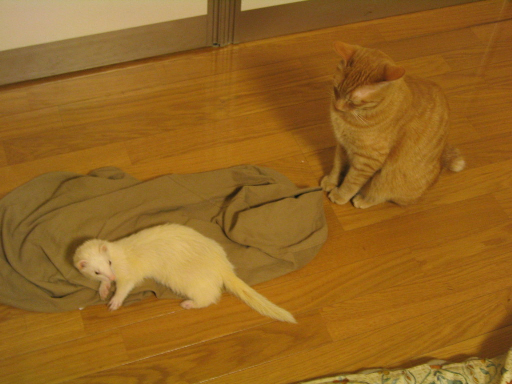
\includegraphics[width=6.4truecm]{./fig/ferret.png}
  \caption{適当なサンプル2}
% \url{http://www.this.is.sample.url/} % Web上のデータの場合、参照先URLを明記
  \label{fig:ferret}
\end{figure}

これまで、\LaTeX での図は伝統的には EPS 形式が用いられてきたが、
近年では JPEG 形式や PNG 形式など多くの画像フォーマットに対応している。
Inkscape や Illustrator 等のように直接 EPS 形式を出力する場合は EPS を用いることが望ましいが、
それ以外の状況では EPS への変換は行わずに画像ファイルを直接指定した方が品質が良い。
ただし、JPEG や PNG などの画像ファイルは EPS に比べて \LaTeX のコンパイルが長時間になる傾向があり、
あまり巨大な画像データを使用するとかなりコンパイル時間が長くなってしまうので、注意が必要である。
また、使用する画像ファイルはこのテンプレートのように
fig サブフォルダ内に格納することを推奨する。

図への参照は \verb+\label+ コマンドを用いて各図のキャプションにキーワードを付けておき、
文中で \verb+\ref+ コマンドによってキーワードを指定することで記述する。
キーワードは参照対象に応じてプリフィクスを付けることが望ましい。
以下の表 \ref{tbl:pre_list} に一般的に用いる参照対象ごとのプリフィクスを挙げる。

\begin{table}[H]
  \caption{ラベルに指定するキーワードのプリフィクス一覧}
  \label{tbl:pre_list}
  \centering
  \begin{tabular}{|l|l|r|} \hline
   参照対象	& プリフィクス \\ \hline
   章		& chp: \\ \hline
   節		& sec: \\ \hline
   図		& fig: \\ \hline
   表 		& tbl: \\ \hline
   式   	& eqn: \\ \hline
  \end{tabular}
\end{table}
手作業でのナンバリングは非効率極まりない上に必ずミスが出るので行わないこと。

\section{\LaTeX のコンパイル}
\LaTeX のコンパイルは、「コマンドプロンプト」や「PowerShell」などのコマンドライン上で「
latexmk」コマンドを用いる。
例えば、「M01xxyyy.tex」というファイルから PDF を作成したい場合は
\begin{verbatim}
    latexmk M01xxyyy
\end{verbatim}
というように、拡張子を抜いてコマンドラインで指定する。

また、コマンドラインに不慣れな学生は、
Atom エディタ等の \LaTeX パッケージを用いることも良案である。
Atom エディタを用いた \LaTeX の記述については、研究室 Wiki を参照のこと。
	
\chapter{まとめ}
\label{chp:first}

近年3Dプリンターの低価格化が進んだことで一般にも普及が進んでいる.
これにより,これまで生産者と消費者は別の者であったが,生産者と消費者が同一の存在となるなりつつあるのだ.
消費者の生産者化により,これまでにない発想の商品が数多く登場し,より便利なこれまでにない発想の商品はデジタル社会により,世界中に拡散され,人類社会の発展に貢献される.
3Dプリンターは人類の可能性を最大化させるためのツールでもある.その3Dプリンターは印刷できる素材が限られているのが現状である.
新たな3Dプリンターの素材を開発することは,多くの人が3Dプリンターを使い新しいものを作り出し、人類の想像力を最大化させるうえで重要なことだと考える.
その中でも,私は氷をマテリアルとした3Dプリンターの開発を行おうと考えた.

氷の彫刻は,世界中で様々なイベントやアート作品に用いられ,多くの人々に親しまれて様々な作品が作られている.
しかし,氷の作品は作るのに時間がかかり,彫刻の技術や設備が必要となるため,誰でも簡単に触れ合えるものではない.
また、現在開発されている氷をマテリアルとした3Dプリンターはマグカップサイズのものを作るのに50時間ほどかかるもなど特殊な環境や知識が必要なものしかない.
そのため,一般の人でも扱いが可能かつ,一般の3Dプリンターと同程度の速度とある程度の精度を両立した氷をマテリアルとした3Dプリンターの提案する.

一般の人でも扱いが可能かつ,一般の3Dプリンターと同程度の速度とある程度の精度を両立した氷をマテリアルとした3Dプリンターを開発するにあたり,
純粋な水を積層すると,水の粘度が低いため,固まる前に広がってしまう.そのため造形精度が悪く,オーバーハングなども造形することが難しい.
よって,水の粘度を上げることにより,上記の問題の解決や精度を向上させることができるのではと考えた.
また,他の研究では,特殊な機材を使用し,装置が高価になりがちである.
日本各地で手に入り,価格も1リットルあたり300円と安価であるため,液体窒素を冷却材として使用する.
最後に一般の人でも扱えるにように,世界中で使用されている3Dプリントおよびスライサーソフトウェアである Ultimaker Cura で操作が可能である必要があると考えると考え,
氷をマテリアルとした3Dプリンターの開発を行った.

実験では,純粋な水を使用した場合と水と砂糖を1:3で混ぜた液体での場合で比較を行った.
水単体と比べ水と砂糖を混ぜた液体での方が造形精度が高く,積層もスムーズに行われた.
氷をマテリアルとした3Dプリンターでの造形を行う際,水と砂糖を混ぜた液体の方が,適しているということが分かった.
また,開発において使用したものは既存の3Dプリンターの部品やどこでも手に入れやすいものを多く使用した.
特に,一般で広く使われているスライサーソフトUltimaker Curaを利用して造形できるため,3Dプリンターを扱えるもの方なら,だれでも操作可能なものになっている.
よって,一般の人でも扱いが可能かつ,一般のユーザーが設計したデータにできるだけ近い形に印刷できる氷をマテリアルとした3Dプリンターの開発ができたと考える.

しかし,今回開発した氷をマテリアルとした3Dプリンターにもいくつか課題が残る.
1つ目が予備実験において,手で試した際の精度を自動かさせた際に再現できていないこと.
2つ目一度に造形できる量に制限があること.
この二つを解決できたらと考える.

今回の研究開発では,氷をマテリアルとした造形物をある程度の速度と精度で制作を行える機構を開発し, Ultimaker Cura で操作可能なプログラムを組むことで既存の氷をマテリアルとした3Dプリンターに比べ,一般の人でも扱いが可能な3Dプリンターになった
水に粘性を持たせることで,一般の3Dプリンターと同程度の速度とある程度の精度を両立した氷をマテリアルとした3Dプリンターに大きく近づくことができた.
しかし,現状のプリンターではまだ,オーバーハングが不十分なこと造形できる量に制限があることなどいくつか問題を抱えている.
また,ノズルのサイズの調整や水の温度の調整,粘度の調整などまだまだ,ある程度の速度と精度をもった3Dプリンターの開発において,検証可能な要素が残されている.
一般の人が気軽に氷の造形を楽しみ,様々な氷の造形物を創造するには,上記の要素の検証を行い,さらなる精度と速度の向上が必要となる.









	
%\chapter{使用例}
\label{chp:first}

\section{段落と改行}
\label{sec:paragraph}

段落頭の字下げは自動で行われるため、全角スペースによる手動調整は不要であり、禁止である。
\LaTeX ソース中での改行は空行を挟まない場合は無視される。
ソース内では自分で編集しやすいように改行してよい。

このように、空行を挟むと改段落となる。
また、強制改行は\\このように \verb+\\+ で強制的に行うことができる。
しかし、この場合は段落の字下げもされないため、改段落を行う用途には空行を用いるべきで、
強制改行(\verb+\\+)は利用すべきではない。

しかしながら、例えば \verb+\verb+ 環境やインライン数式を用いる場合などで、
\verb+abcdefghijklmnopqrstuvwxyzABCDEFGHIJKLMNOPQRSTUVWXYZ+ 
というようにページ幅を超えてしまったり、前の行が間延びしてしまうようなケースがある。
そのような場合、\verb+\\+ を用いて強制改行により \\
\verb+abcdefghijklmnopqrstuvwxyzABCDEFGHIJKLMNOPQRSTUVWXYZ+ 
というように用いるとよい。

\section{箇条書き}
\label{sec:enum}

数字を使った場合の箇条書きの例を示す。

\begin{enumerate}
 \item 数字の付いた箇条書きの例
 \item こんな感じで手順などを列挙
\end{enumerate}

数字を付けずに列挙したい場合は itemize 環境を使う。
このようにあるキーワードを指定して \verb+\begin(}+ と \verb+\end{}+ で
囲む範囲のことを○○環境と呼ぶ。

\begin{itemize}
 \item 順番などを伴わない箇条書きの例
 \item 材料や要素を純粋に列挙したい場合に使用
\end{itemize}

enumerate 環境や itemize 環境は、入れ子構造を持つことができる。
例えば enumerate 環境の場合、以下のようになる。
\begin{enumerate}
 \item 東京都
 \begin{enumerate}
  \item 八王子市
  \item 多摩市
 \end{enumerate}
 \item 神奈川県
 \begin{enumerate}
  \item 横浜市
  \item 川崎市
 \end{enumerate}
 \item 山梨県
\end{enumerate}

\section{図表と参照}
\label{sec:fig_tbl}

図を挿入する際は以下のように書く。
必ずキャプションを付けるとともに、図に対する説明を本文中で記載すること。
何かの手違いで図が表示されなくなったとしても、文章で意味が通じるくらいに説明するのを目安にすること。
以下の図 \ref{fig:sample} と図 \ref{fig:ferret} は、適当なサンプル画像である。

\begin{figure}[H]
  \centering
  
\includegraphics[width=6.4cm]{./fig/fig-sample.eps}
  \caption{適当なサンプル}
% \url{http://www.this.is.sample.url/} % Web上のデータの場合、参照先URLを明記
  \label{fig:sample}
\end{figure}

\begin{figure}[H]
  \centering
  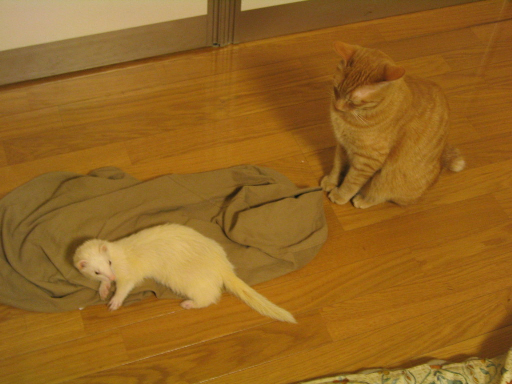
\includegraphics[width=6.4truecm]{./fig/ferret.png}
  \caption{適当なサンプル2}
% \url{http://www.this.is.sample.url/} % Web上のデータの場合、参照先URLを明記
  \label{fig:ferret}
\end{figure}

これまで、\LaTeX での図は伝統的には EPS 形式が用いられてきたが、
近年では JPEG 形式や PNG 形式など多くの画像フォーマットに対応している。
Inkscape や Illustrator 等のように直接 EPS 形式を出力する場合は EPS を用いることが望ましいが、
それ以外の状況では EPS への変換は行わずに画像ファイルを直接指定した方が品質が良い。
ただし、JPEG や PNG などの画像ファイルは EPS に比べて \LaTeX のコンパイルが長時間になる傾向があり、
あまり巨大な画像データを使用するとかなりコンパイル時間が長くなってしまうので、注意が必要である。
また、使用する画像ファイルはこのテンプレートのように
fig サブフォルダ内に格納することを推奨する。

図への参照は \verb+\label+ コマンドを用いて各図のキャプションにキーワードを付けておき、
文中で \verb+\ref+ コマンドによってキーワードを指定することで記述する。
キーワードは参照対象に応じてプリフィクスを付けることが望ましい。
以下の表 \ref{tbl:pre_list} に一般的に用いる参照対象ごとのプリフィクスを挙げる。

\begin{table}[H]
  \caption{ラベルに指定するキーワードのプリフィクス一覧}
  \label{tbl:pre_list}
  \centering
  \begin{tabular}{|l|l|r|} \hline
   参照対象	& プリフィクス \\ \hline
   章		& chp: \\ \hline
   節		& sec: \\ \hline
   図		& fig: \\ \hline
   表 		& tbl: \\ \hline
   式   	& eqn: \\ \hline
  \end{tabular}
\end{table}
手作業でのナンバリングは非効率極まりない上に必ずミスが出るので行わないこと。

\section{\LaTeX のコンパイル}
\LaTeX のコンパイルは、「コマンドプロンプト」や「PowerShell」などのコマンドライン上で「
latexmk」コマンドを用いる。
例えば、「M01xxyyy.tex」というファイルから PDF を作成したい場合は
\begin{verbatim}
    latexmk M01xxyyy
\end{verbatim}
というように、拡張子を抜いてコマンドラインで指定する。

また、コマンドラインに不慣れな学生は、
Atom エディタ等の \LaTeX パッケージを用いることも良案である。
Atom エディタを用いた \LaTeX の記述については、研究室 Wiki を参照のこと。

%\chapter{今後の展望}
\label{chp:first}

\section{段落と改行}
\label{sec:paragraph}

段落頭の字下げは自動で行われるため、全角スペースによる手動調整は不要であり、禁止である。
\LaTeX ソース中での改行は空行を挟まない場合は無視される。
ソース内では自分で編集しやすいように改行してよい。

このように、空行を挟むと改段落となる。
また、強制改行は\\このように \verb+\\+ で強制的に行うことができる。
しかし、この場合は段落の字下げもされないため、改段落を行う用途には空行を用いるべきで、
強制改行(\verb+\\+)は利用すべきではない。

しかしながら、例えば \verb+\verb+ 環境やインライン数式を用いる場合などで、
\verb+abcdefghijklmnopqrstuvwxyzABCDEFGHIJKLMNOPQRSTUVWXYZ+ 
というようにページ幅を超えてしまったり、前の行が間延びしてしまうようなケースがある。
そのような場合、\verb+\\+ を用いて強制改行により \\
\verb+abcdefghijklmnopqrstuvwxyzABCDEFGHIJKLMNOPQRSTUVWXYZ+ 
というように用いるとよい。

\section{箇条書き}
\label{sec:enum}

数字を使った場合の箇条書きの例を示す。

\begin{enumerate}
 \item 数字の付いた箇条書きの例
 \item こんな感じで手順などを列挙
\end{enumerate}

数字を付けずに列挙したい場合は itemize 環境を使う。
このようにあるキーワードを指定して \verb+\begin(}+ と \verb+\end{}+ で
囲む範囲のことを○○環境と呼ぶ。

\begin{itemize}
 \item 順番などを伴わない箇条書きの例
 \item 材料や要素を純粋に列挙したい場合に使用
\end{itemize}

enumerate 環境や itemize 環境は、入れ子構造を持つことができる。
例えば enumerate 環境の場合、以下のようになる。
\begin{enumerate}
 \item 東京都
 \begin{enumerate}
  \item 八王子市
  \item 多摩市
 \end{enumerate}
 \item 神奈川県
 \begin{enumerate}
  \item 横浜市
  \item 川崎市
 \end{enumerate}
 \item 山梨県
\end{enumerate}

\section{図表と参照}
\label{sec:fig_tbl}

図を挿入する際は以下のように書く。
必ずキャプションを付けるとともに、図に対する説明を本文中で記載すること。
何かの手違いで図が表示されなくなったとしても、文章で意味が通じるくらいに説明するのを目安にすること。
以下の図 \ref{fig:sample} と図 \ref{fig:ferret} は、適当なサンプル画像である。

\begin{figure}[H]
  \centering
  
\includegraphics[width=6.4cm]{./fig/fig-sample.eps}
  \caption{適当なサンプル}
% \url{http://www.this.is.sample.url/} % Web上のデータの場合、参照先URLを明記
  \label{fig:sample}
\end{figure}

\begin{figure}[H]
  \centering
  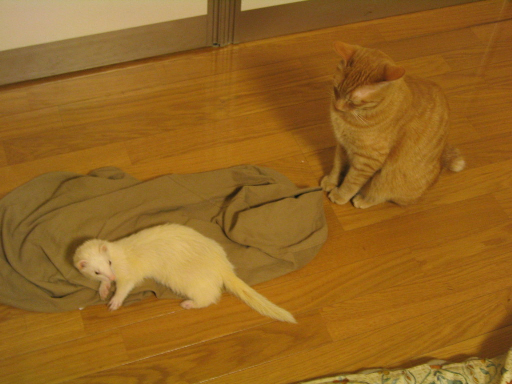
\includegraphics[width=6.4truecm]{./fig/ferret.png}
  \caption{適当なサンプル2}
% \url{http://www.this.is.sample.url/} % Web上のデータの場合、参照先URLを明記
  \label{fig:ferret}
\end{figure}

これまで、\LaTeX での図は伝統的には EPS 形式が用いられてきたが、
近年では JPEG 形式や PNG 形式など多くの画像フォーマットに対応している。
Inkscape や Illustrator 等のように直接 EPS 形式を出力する場合は EPS を用いることが望ましいが、
それ以外の状況では EPS への変換は行わずに画像ファイルを直接指定した方が品質が良い。
ただし、JPEG や PNG などの画像ファイルは EPS に比べて \LaTeX のコンパイルが長時間になる傾向があり、
あまり巨大な画像データを使用するとかなりコンパイル時間が長くなってしまうので、注意が必要である。
また、使用する画像ファイルはこのテンプレートのように
fig サブフォルダ内に格納することを推奨する。

図への参照は \verb+\label+ コマンドを用いて各図のキャプションにキーワードを付けておき、
文中で \verb+\ref+ コマンドによってキーワードを指定することで記述する。
キーワードは参照対象に応じてプリフィクスを付けることが望ましい。
以下の表 \ref{tbl:pre_list} に一般的に用いる参照対象ごとのプリフィクスを挙げる。

\begin{table}[H]
  \caption{ラベルに指定するキーワードのプリフィクス一覧}
  \label{tbl:pre_list}
  \centering
  \begin{tabular}{|l|l|r|} \hline
   参照対象	& プリフィクス \\ \hline
   章		& chp: \\ \hline
   節		& sec: \\ \hline
   図		& fig: \\ \hline
   表 		& tbl: \\ \hline
   式   	& eqn: \\ \hline
  \end{tabular}
\end{table}
手作業でのナンバリングは非効率極まりない上に必ずミスが出るので行わないこと。

\section{\LaTeX のコンパイル}
\LaTeX のコンパイルは、「コマンドプロンプト」や「PowerShell」などのコマンドライン上で「
latexmk」コマンドを用いる。
例えば、「M01xxyyy.tex」というファイルから PDF を作成したい場合は
\begin{verbatim}
    latexmk M01xxyyy
\end{verbatim}
というように、拡張子を抜いてコマンドラインで指定する。

また、コマンドラインに不慣れな学生は、
Atom エディタ等の \LaTeX パッケージを用いることも良案である。
Atom エディタを用いた \LaTeX の記述については、研究室 Wiki を参照のこと。
		% 第1章	
%\chapter{その次}
\label{chp:second}

\section{数式}
\label{sec:eqn}

数式のインラインモードは \(x^2 + y^2 \leq 1\) のように表示させることができる.
インラインモードで「\verb+$...$+」を使うやり方は,
近年の LaTeX ではあまり推奨されていないが,その利用は妨げない.

ディスプレイ数式モードを利用する際に推奨するのは equation 環境である.
\begin{equation}
	\mathbf{A}_p = \frac{\mathbf{A}\cdot\mathbf{B}}{|\mathbf{B}|^2}\mathbf{B} .
	\label{eq:samp1}
\end{equation}
数式の参照は「\verb+\ref+」ではなく「\verb+\eqref+」を用いる.
上記の数式を参照すると「式\eqref{eq:samp1}」となる.
このように,\verb+\eqref+ を用いた場合は数式中と同じ様式の括弧がつく.

また,複数行にわたる数式を表示したい場合は align 環境を用いることを推奨する.
以下の式\eqref{eq:samp2}にその例を示す.

\begin{align}
	& \begin{bmatrix}
	a_{11} & a_{12} & \cdots & a_{1n} \\
	a_{21} & a_{22} & \cdots & a_{2n} \\
	\vdots & \vdots & \ddots & \vdots \\
	a_{m1} & a_{m2} & \cdots & a_{mn} \\
	\end{bmatrix}
	\otimes
	\begin{bmatrix}
	b_{11} & b_{12} & \cdots & b_{1n} \\
	b_{21} & b_{22} & \cdots & b_{2n} \\
	\vdots & \vdots & \ddots & \vdots \\
	b_{m1} & b_{m2} & \cdots & b_{mn} \\
	\end{bmatrix} \notag \\
	& \qquad \qquad = \sum_{i}^{m}\sum_{j}^{n}a_{ij}b_{ij} .
	\label{eq:samp2}
\end{align}

数式で複数行を用いる方法として、古い \LaTeX に関する資料では eqnarray 環境の
解説を行っている場合があるが、最近の \LaTeX では幾つかのパッケージ
(特に\AmS 関連)と同時に利用すると問題が発生することがあるため、利用は推奨しない.
複数行を用いる方法としては他にも gather, multline, split など多くの環境があるが、
equnarray 以外のものであれば問題はない。

具体的な数式の記述方法については書籍や Web 上の情報等を参照のこと。

\section{寸法}

\LaTeX では、縦方向や横方向に空白を空けたいとき (\verb+\vspace+, \verb+\hspace+) や、
画像の縦幅や横幅を指定したい場合など、多くの場面で寸法を指定することがある。
\LaTeX の寸法単位は mm (ミリメートル) や cm (センチメートル) など多くの種類が利用でき、
小数点以下も記述できるためかなり柔軟な指定ができる。例えば、表のキャプションと
本体の間を少し空けたいときは
\begin{verbatim}
\begin{table}[H]
  \caption{ラベルに指定するキーワードのプリフィクス一覧}
  \label{tbl:pre_list}
  \centering
  \vspace{0.5cm}
  \begin{tabular}{|l|l|r|} \hline
\end{verbatim}
のように、表本体の直前に \verb+\vspace+ を入れればよい。

\LaTeX の寸法指定で留意すべきこととして、単位の「true つき」と「true なし」の使い分けがある。
例えば、先述の「\verb+\vspace{0.5cm}+」に対し、true つきの場合は
「\verb+\vspace{0.5truecm}+」ということになる。

true がついていない場合、\verb+\documentclass+ の指定時でのフォントサイズを変更すると、
そのフォントサイズに伴って(空白幅や画像幅などの)実際の寸法も変化する。
フォントサイズを変更した際に連動してほしい寸法については、この「true なし」を用いるとよい。
一方、「true つき」の場合はフォントサイズの変更には連動せず常に固定の値となる。
センタリングした画像幅などはフォントサイズと連動しない方が都合がよいことも多く、
そういった場合は「true つき」の寸法を指定するとよい。

\section{参考文献}
\label{sec:bib}

参考文献リストの作成は、\BibTeX を用いることを推奨する。
文献の参照は、リスト上で文献に付けたキーワードをciteコマンドによって指定することで記述する。
例えば、
「阿部ら\cite{abeJ}によると、
某手法\cite{nowrouzezahrai}には重大な欠点が存在することが指摘されている。」
という利用方法となる。

文献を1つも参照していない状態でPDFを生成するバッチファイルを実行するとエラーとなるので注意すること。
生成したPDFファイル中で参照がうまくできていない場合には参照番号ではなく
「\verb+?+」記号が表示される。

\BibTeX の記述方法は、どのような種類の文献かによって異なる。以下に具体的な例を列挙する。
\begin{itemize}
 \item 論文誌掲載の学術論文\cite{abeJ}\cite{nowrouzezahrai}
 \item 研究会の研究報告\cite{aoki}
 \item 博士論文\cite{takeuchi}
 \item 修士論文\cite{abeM}
 \item 学部卒業論文\cite{abeU}
 \item 書籍\cite{dragonball}
 \item URL\cite{effekseer}
\end{itemize}

文献の属性の種類や、設定するべきステータスについてもWebを参照すること。
論文データベースサイトでは \BibTeX の記述形式によるテキストを出力してくれるところもあるので、
利用できると便利である。
リストの記述順は一切気にする必要がなく、
参考文献に挙げないものが含まれていても問題無いので、関連しそうな文献は全てリスト化しておくとよい。

\BibTeX における著者名の列挙はカンマで並べるのではなく、
\begin{verbatim}
    author = "阿部 雅樹 and 渡辺 大地 and 三上 浩司",
\end{verbatim}
というように、各氏名の間に「and」を入れるという独特の形式を持つ。

また、\BibTeX では author や title 等での
アルファベット大文字小文字を自動的に変換する機能があり、
例えばタイトル中の「3DCG における」といった文字列は「3dcg における」となる。
これを強制的に大文字小文字を指定したい場合は、
\begin{verbatim}
    title = "{3DCG}における何かしらの手法",
\end{verbatim}
のようにその部分だけ波括弧で囲うことで指定できる。

	

\delchapnumber
\chapter{謝辞}
\label{chp:thanks}

謝辞は基本的に査読の対象とならない。各人の自由に記述して良い。
ただし、あまりに公序良俗に反する内容である場合は修正を求める場合があるので、
はっちゃけるにしても良識・常識の範疇を超えないようにして欲しい。
			% 謝辞
\bibliography{BibTeX}		% BibTeXを使う場合の参考文献リスト
\bibliographystyle{junsrt}	% BibTeXを使う場合のスタイル
\undochapnumber
\appendix			% 付録 (もしあれば)
\chapter{ }
\label{chp:first}
本研究のために書き換えた3DプリンターのファームウエアMariln内にある,変更ファイルConfiguration.hのコードである. 



\begin{lstlisting}



  /**
 * Marlin 3D Printer Firmware
 * Copyright (C) 2016 MarlinFirmware [https://github.com/MarlinFirmware/Marlin]
 *
 * Based on Sprinter and grbl.
 * Copyright (C) 2011 Camiel Gubbels / Erik van der Zalm
 *
 * This program is free software: you can redistribute it and/or modify
 * it under the terms of the GNU General Public License as published by
 * the Free Software Foundation, either version 3 of the License, or
 * (at your option) any later version.
 *
 * This program is distributed in the hope that it will be useful,
 * but WITHOUT ANY WARRANTY; without even the implied warranty of
 * MERCHANTABILITY or FITNESS FOR A PARTICULAR PURPOSE.  See the
 * GNU General Public License for more details.
 *
 * You should have received a copy of the GNU General Public License
 * along with this program.  If not, see <http://www.gnu.org/licenses/>.
 *
 */

/**
 * Configuration.h
 *
 * Basic settings such as:
 *
 * - Type of electronics
 * - Type of temperature sensor
 * - Printer geometry
 * - Endstop configuration
 * - LCD controller
 * - Extra features
 *
 * Advanced settings can be found in Configuration_adv.h
 *
 */
#ifndef CONFIGURATION_H
#define CONFIGURATION_H
#define CONFIGURATION_H_VERSION 010109

//===========================================================================
//============================= Getting Started =============================
//===========================================================================

/**
 * Here are some standard links for getting your machine calibrated:
 *
 * http://reprap.org/wiki/Calibration
 * http://youtu.be/wAL9d7FgInk
 * http://calculator.josefprusa.cz
 * http://reprap.org/wiki/Triffid_Hunter%27s_Calibration_Guide
 * http://www.thingiverse.com/thing:5573
 * https://sites.google.com/site/repraplogphase/calibration-of-your-reprap
 * http://www.thingiverse.com/thing:298812
 */

//===========================================================================
//============================= DELTA Printer ===============================
//===========================================================================
// For a Delta printer start with one of the configuration files in the
// example_configurations/delta directory and customize for your machine.
//

//===========================================================================
//============================= SCARA Printer ===============================
//===========================================================================
// For a SCARA printer start with the configuration files in
// example_configurations/SCARA and customize for your machine.
//

//===========================================================================
//============================= HANGPRINTER =================================
//===========================================================================
// For a Hangprinter start with the configuration file in the
// example_configurations/hangprinter directory and customize for your machine.
//

// @section info

// User-specified version info of this build to display in [Pronterface, etc] terminal window during
// startup. Implementation of an idea by Prof Braino to inform user that any changes made to this
// build by the user have been successfully uploaded into firmware.
#define STRING_CONFIG_H_AUTHOR "(davidramiro)" // Who made the changes.
#define SHOW_BOOTSCREEN
#define STRING_SPLASH_LINE1 SHORT_BUILD_VERSION   // will be shown during bootup in line 1
#define STRING_SPLASH_LINE2 CUSTOM_BUILD_VERSION  // will be shown during bootup in line 2

/**
 * *** VENDORS PLEASE READ ***
 *
 * Marlin allows you to add a custom boot image for Graphical LCDs.
 * With this option Marlin will first show your custom screen followed
 * by the standard Marlin logo with version number and web URL.
 *
 * We encourage you to take advantage of this new feature and we also
 * respectfully request that you retain the unmodified Marlin boot screen.
 */

// Enable to show the bitmap in Marlin/_Bootscreen.h on startup.
//#define SHOW_CUSTOM_BOOTSCREEN

// Enable to show the bitmap in Marlin/_Statusscreen.h on the status screen.
//#define CUSTOM_STATUS_SCREEN_IMAGE

// @section machine

/**
 * Select the serial port on the board to use for communication with the host.
 * This allows the connection of wireless adapters (for instance) to non-default port pins.
 * Serial port 0 is always used by the Arduino bootloader regardless of this setting.
 *
 * :[0, 1, 2, 3, 4, 5, 6, 7]
 */
#define SERIAL_PORT 0

/**
 * This setting determines the communication speed of the printer.
 *
 * 250000 works in most cases, but you might try a lower speed if
 * you commonly experience drop-outs during host printing.
 * You may try up to 1000000 to speed up SD file transfer.
 *
 * :[2400, 9600, 19200, 38400, 57600, 115200, 250000, 500000, 1000000]
 */
#define BAUDRATE 250000

// Enable the Bluetooth serial interface on AT90USB devices
//#define BLUETOOTH

// The following define selects which electronics board you have.
// Please choose the name from boards.h that matches your setup
#ifndef MOTHERBOARD
  #define MOTHERBOARD BOARD_TRIGORILLA_14
#endif

// Optional custom name for your RepStrap or other custom machine
// Displayed in the LCD "Ready" message
//#define CUSTOM_MACHINE_NAME "3D Printer"

// Define this to set a unique identifier for this printer, (Used by some programs to differentiate between machines)
// You can use an online service to generate a random UUID. (eg http://www.uuidgenerator.net/version4)
//#define MACHINE_UUID "00000000-0000-0000-0000-000000000000"

// @section extruder

// This defines the number of extruders
// :[1, 2, 3, 4, 5]
#define EXTRUDERS 1

// Generally expected filament diameter (1.75, 2.85, 3.0, ...). Used for Volumetric, Filament Width Sensor, etc.
#define DEFAULT_NOMINAL_FILAMENT_DIA 1.75

// For Cyclops or any "multi-extruder" that shares a single nozzle.
//#define SINGLENOZZLE

/**
 * Prusa MK2 Single Nozzle Multi-Material Multiplexer, and variants.
 *
 * This device allows one stepper driver on a control board to drive
 * two to eight stepper motors, one at a time, in a manner suitable
 * for extruders.
 *
 * This option only allows the multiplexer to switch on tool-change.
 * Additional options to configure custom E moves are pending.
 */
//#define MK2_MULTIPLEXER
#if ENABLED(MK2_MULTIPLEXER)
  // Override the default DIO selector pins here, if needed.
  // Some pins files may provide defaults for these pins.
  //#define E_MUX0_PIN 40  // Always Required
  //#define E_MUX1_PIN 42  // Needed for 3 to 8 steppers
  //#define E_MUX2_PIN 44  // Needed for 5 to 8 steppers
#endif

// A dual extruder that uses a single stepper motor
//#define SWITCHING_EXTRUDER
#if ENABLED(SWITCHING_EXTRUDER)
  #define SWITCHING_EXTRUDER_SERVO_NR 0
  #define SWITCHING_EXTRUDER_SERVO_ANGLES { 0, 90 } // Angles for E0, E1[, E2, E3]
  #if EXTRUDERS > 3
    #define SWITCHING_EXTRUDER_E23_SERVO_NR 1
  #endif
#endif

// A dual-nozzle that uses a servomotor to raise/lower one of the nozzles
//#define SWITCHING_NOZZLE
#if ENABLED(SWITCHING_NOZZLE)
  #define SWITCHING_NOZZLE_SERVO_NR 0
  #define SWITCHING_NOZZLE_SERVO_ANGLES { 0, 90 }   // Angles for E0, E1
  //#define HOTEND_OFFSET_Z { 0.0, 0.0 }
#endif

/**
 * Two separate X-carriages with extruders that connect to a moving part
 * via a magnetic docking mechanism. Requires SOL1_PIN and SOL2_PIN.
 */
//#define PARKING_EXTRUDER
#if ENABLED(PARKING_EXTRUDER)
  #define PARKING_EXTRUDER_SOLENOIDS_INVERT           // If enabled, the solenoid is NOT magnetized with applied voltage
  #define PARKING_EXTRUDER_SOLENOIDS_PINS_ACTIVE LOW  // LOW or HIGH pin signal energizes the coil
  #define PARKING_EXTRUDER_SOLENOIDS_DELAY 250        // Delay (ms) for magnetic field. No delay if 0 or not defined.
  #define PARKING_EXTRUDER_PARKING_X { -78, 184 }     // X positions for parking the extruders
  #define PARKING_EXTRUDER_GRAB_DISTANCE 1            // mm to move beyond the parking point to grab the extruder
  #define PARKING_EXTRUDER_SECURITY_RAISE 5           // Z-raise before parking
  #define HOTEND_OFFSET_Z { 0.0, 1.3 }                // Z-offsets of the two hotends. The first must be 0.
#endif

/**
 * "Mixing Extruder"
 *   - Adds G-codes M163 and M164 to set and "commit" the current mix factors.
 *   - Extends the stepping routines to move multiple steppers in proportion to the mix.
 *   - Optional support for Repetier Firmware's 'M164 S<index>' supporting virtual tools.
 *   - This implementation supports up to two mixing extruders.
 *   - Enable DIRECT_MIXING_IN_G1 for M165 and mixing in G1 (from Pia Taubert's reference implementation).
 */
//#define MIXING_EXTRUDER
#if ENABLED(MIXING_EXTRUDER)
  #define MIXING_STEPPERS 2        // Number of steppers in your mixing extruder
  #define MIXING_VIRTUAL_TOOLS 16  // Use the Virtual Tool method with M163 and M164
  //#define DIRECT_MIXING_IN_G1    // Allow ABCDHI mix factors in G1 movement commands
#endif

// Offset of the extruders (uncomment if using more than one and relying on firmware to position when changing).
// The offset has to be X=0, Y=0 for the extruder 0 hotend (default extruder).
// For the other hotends it is their distance from the extruder 0 hotend.
//#define HOTEND_OFFSET_X {0.0, 20.00} // (in mm) for each extruder, offset of the hotend on the X axis
//#define HOTEND_OFFSET_Y {0.0, 5.00}  // (in mm) for each extruder, offset of the hotend on the Y axis

// @section machine

/**
 * Select your power supply here. Use 0 if you haven't connected the PS_ON_PIN
 *
 * 0 = No Power Switch
 * 1 = ATX
 * 2 = X-Box 360 203Watts (the blue wire connected to PS_ON and the red wire to VCC)
 *
 * :{ 0:'No power switch', 1:'ATX', 2:'X-Box 360' }
 */
#define POWER_SUPPLY 0

#if POWER_SUPPLY > 0
  // Enable this option to leave the PSU off at startup.
  // Power to steppers and heaters will need to be turned on with M80.
  //#define PS_DEFAULT_OFF

  //#define AUTO_POWER_CONTROL        // Enable automatic control of the PS_ON pin
  #if ENABLED(AUTO_POWER_CONTROL)
    #define AUTO_POWER_FANS           // Turn on PSU if fans need power
    #define AUTO_POWER_E_FANS
    #define AUTO_POWER_CONTROLLERFAN
    #define POWER_TIMEOUT 30
  #endif

#endif

// @section temperature

//===========================================================================
//============================= Thermal Settings ============================
//===========================================================================

/**
 * --NORMAL IS 4.7kohm PULLUP!-- 1kohm pullup can be used on hotend sensor, using correct resistor and table
 *
 * Temperature sensors available:
 *
 *    -4 : thermocouple with AD8495
 *    -3 : thermocouple with MAX31855 (only for sensor 0)
 *    -2 : thermocouple with MAX6675 (only for sensor 0)
 *    -1 : thermocouple with AD595
 *     0 : not used
 *     1 : 100k thermistor - best choice for EPCOS 100k (4.7k pullup)
 *     2 : 200k thermistor - ATC Semitec 204GT-2 (4.7k pullup)
 *     3 : Mendel-parts thermistor (4.7k pullup)
 *     4 : 10k thermistor !! do not use it for a hotend. It gives bad resolution at high temp. !!
 *     5 : 100K thermistor - ATC Semitec 104GT-2/104NT-4-R025H42G (Used in ParCan & J-Head) (4.7k pullup)
 *   501 : 100K Zonestar (Tronxy X3A) Thermistor
 *     6 : 100k EPCOS - Not as accurate as table 1 (created using a fluke thermocouple) (4.7k pullup)
 *     7 : 100k Honeywell thermistor 135-104LAG-J01 (4.7k pullup)
 *    71 : 100k Honeywell thermistor 135-104LAF-J01 (4.7k pullup)
 *     8 : 100k 0603 SMD Vishay NTCS0603E3104FXT (4.7k pullup)
 *     9 : 100k GE Sensing AL03006-58.2K-97-G1 (4.7k pullup)
 *    10 : 100k RS thermistor 198-961 (4.7k pullup)
 *    11 : 100k beta 3950 1% thermistor (4.7k pullup)
 *    12 : 100k 0603 SMD Vishay NTCS0603E3104FXT (4.7k pullup) (calibrated for Makibox hot bed)
 *    13 : 100k Hisens 3950  1% up to 300°C for hotend "Simple ONE " & "Hotend "All In ONE"
 *    15 : 100k thermistor calibration for JGAurora A5 hotend
 *    20 : the PT100 circuit found in the Ultimainboard V2.x
 *    60 : 100k Maker's Tool Works Kapton Bed Thermistor beta=3950
 *    66 : 4.7M High Temperature thermistor from Dyze Design
 *    70 : the 100K thermistor found in the bq Hephestos 2
 *    75 : 100k Generic Silicon Heat Pad with NTC 100K MGB18-104F39050L32 thermistor
 *
 *       1k ohm pullup tables - This is atypical, and requires changing out the 4.7k pullup for 1k.
 *                              (but gives greater accuracy and more stable PID)
 *    51 : 100k thermistor - EPCOS (1k pullup)
 *    52 : 200k thermistor - ATC Semitec 204GT-2 (1k pullup)
 *    55 : 100k thermistor - ATC Semitec 104GT-2 (Used in ParCan & J-Head) (1k pullup)
 *
 *  1047 : Pt1000 with 4k7 pullup
 *  1010 : Pt1000 with 1k pullup (non standard)
 *   147 : Pt100 with 4k7 pullup
 *   110 : Pt100 with 1k pullup (non standard)
 *
 *         Use these for Testing or Development purposes. NEVER for production machine.
 *   998 : Dummy Table that ALWAYS reads 25°C or the temperature defined below.
 *   999 : Dummy Table that ALWAYS reads 100°C or the temperature defined below.
 *
 * :{ '0': "Not used", '1':"100k / 4.7k - EPCOS", '2':"200k / 4.7k - ATC Semitec 204GT-2", '3':"Mendel-parts / 4.7k", '4':"10k !! do not use for a hotend. Bad resolution at high temp. !!", '5':"100K / 4.7k - ATC Semitec 104GT-2 (Used in ParCan & J-Head)", '501':"100K Zonestar (Tronxy X3A)", '6':"100k / 4.7k EPCOS - Not as accurate as Table 1", '7':"100k / 4.7k Honeywell 135-104LAG-J01", '8':"100k / 4.7k 0603 SMD Vishay NTCS0603E3104FXT", '9':"100k / 4.7k GE Sensing AL03006-58.2K-97-G1", '10':"100k / 4.7k RS 198-961", '11':"100k / 4.7k beta 3950 1%", '12':"100k / 4.7k 0603 SMD Vishay NTCS0603E3104FXT (calibrated for Makibox hot bed)", '13':"100k Hisens 3950  1% up to 300°C for hotend 'Simple ONE ' & hotend 'All In ONE'", '20':"PT100 (Ultimainboard V2.x)", '51':"100k / 1k - EPCOS", '52':"200k / 1k - ATC Semitec 204GT-2", '55':"100k / 1k - ATC Semitec 104GT-2 (Used in ParCan & J-Head)", '60':"100k Maker's Tool Works Kapton Bed Thermistor beta=3950", '66':"Dyze Design 4.7M High Temperature thermistor", '70':"the 100K thermistor found in the bq Hephestos 2", '71':"100k / 4.7k Honeywell 135-104LAF-J01", '147':"Pt100 / 4.7k", '1047':"Pt1000 / 4.7k", '110':"Pt100 / 1k (non-standard)", '1010':"Pt1000 / 1k (non standard)", '-4':"Thermocouple + AD8495", '-3':"Thermocouple + MAX31855 (only for sensor 0)", '-2':"Thermocouple + MAX6675 (only for sensor 0)", '-1':"Thermocouple + AD595",'998':"Dummy 1", '999':"Dummy 2" }
 */
#define TEMP_SENSOR_0 5
#define TEMP_SENSOR_1 0
#define TEMP_SENSOR_2 0
#define TEMP_SENSOR_3 0
#define TEMP_SENSOR_4 0
#define TEMP_SENSOR_BED 1
#define TEMP_SENSOR_CHAMBER 0

// Dummy thermistor constant temperature readings, for use with 998 and 999
#define DUMMY_THERMISTOR_998_VALUE 25
#define DUMMY_THERMISTOR_999_VALUE 100

// Use temp sensor 1 as a redundant sensor with sensor 0. If the readings
// from the two sensors differ too much the print will be aborted.
//#define TEMP_SENSOR_1_AS_REDUNDANT
#define MAX_REDUNDANT_TEMP_SENSOR_DIFF 10

// Extruder temperature must be close to target for this long before M109 returns success
#define TEMP_RESIDENCY_TIME 10  // (seconds)
#define TEMP_HYSTERESIS 3       // (degC) range of +/- temperatures considered "close" to the target one
#define TEMP_WINDOW     1       // (degC) Window around target to start the residency timer x degC early.

// Bed temperature must be close to target for this long before M190 returns success
#define TEMP_BED_RESIDENCY_TIME 10  // (seconds)
#define TEMP_BED_HYSTERESIS 3       // (degC) range of +/- temperatures considered "close" to the target one
#define TEMP_BED_WINDOW     1       // (degC) Window around target to start the residency timer x degC early.

// The minimal temperature defines the temperature below which the heater will not be enabled It is used
// to check that the wiring to the thermistor is not broken.
// Otherwise this would lead to the heater being powered on all the time.
#define HEATER_0_MINTEMP 5
#define HEATER_1_MINTEMP 5
#define HEATER_2_MINTEMP 5
#define HEATER_3_MINTEMP 5
#define HEATER_4_MINTEMP 5
#define BED_MINTEMP 5

// When temperature exceeds max temp, your heater will be switched off.
// This feature exists to protect your hotend from overheating accidentally, but *NOT* from thermistor short/failure!
// You should use MINTEMP for thermistor short/failure protection.
#define HEATER_0_MAXTEMP 285
#define HEATER_1_MAXTEMP 275
#define HEATER_2_MAXTEMP 275
#define HEATER_3_MAXTEMP 275
#define HEATER_4_MAXTEMP 275
#define BED_MAXTEMP 135

//===========================================================================
//============================= PID Settings ================================
//===========================================================================
// PID Tuning Guide here: http://reprap.org/wiki/PID_Tuning

// Comment the following line to disable PID and enable bang-bang.
#define PIDTEMP
#define BANG_MAX 255     // Limits current to nozzle while in bang-bang mode; 255=full current
#define PID_MAX BANG_MAX // Limits current to nozzle while PID is active (see PID_FUNCTIONAL_RANGE below); 255=full current
#define PID_K1 0.95      // Smoothing factor within any PID loop
#if ENABLED(PIDTEMP)
  //#define PID_AUTOTUNE_MENU // Add PID Autotune to the LCD "Temperature" menu to run M303 and apply the result.
  //#define PID_DEBUG // Sends debug data to the serial port.
  //#define PID_OPENLOOP 1 // Puts PID in open loop. M104/M140 sets the output power from 0 to PID_MAX
  //#define SLOW_PWM_HEATERS // PWM with very low frequency (roughly 0.125Hz=8s) and minimum state time of approximately 1s useful for heaters driven by a relay
  //#define PID_PARAMS_PER_HOTEND // Uses separate PID parameters for each extruder (useful for mismatched extruders)
                                  // Set/get with gcode: M301 E[extruder number, 0-2]
  #define PID_FUNCTIONAL_RANGE 10 // If the temperature difference between the target temperature and the actual temperature
                                  // is more than PID_FUNCTIONAL_RANGE then the PID will be shut off and the heater will be set to min/max.

  // If you are using a pre-configured hotend then you can use one of the value sets by uncommenting it

  // i3 Mega stock v5 hotend, 40W heater cartridge (3.6Ω @ 22°C)
  #define  DEFAULT_Kp 15.94
  #define  DEFAULT_Ki 1.17
  #define  DEFAULT_Kd 54.19

  // Ultimaker
  //#define  DEFAULT_Kp 22.2
  //#define  DEFAULT_Ki 1.08
  //#define  DEFAULT_Kd 114

  // MakerGear
  //#define DEFAULT_Kp 7.0
  //#define DEFAULT_Ki 0.1
  //#define DEFAULT_Kd 12

  // Mendel Parts V9 on 12V
  //#define DEFAULT_Kp 63.0
  //#define DEFAULT_Ki 2.25
  //#define DEFAULT_Kd 440

#endif // PIDTEMP

//===========================================================================
//============================= PID > Bed Temperature Control ===============
//===========================================================================

/**
 * PID Bed Heating
 *
 * If this option is enabled set PID constants below.
 * If this option is disabled, bang-bang will be used and BED_LIMIT_SWITCHING will enable hysteresis.
 *
 * The PID frequency will be the same as the extruder PWM.
 * If PID_dT is the default, and correct for the hardware/configuration, that means 7.689Hz,
 * which is fine for driving a square wave into a resistive load and does not significantly
 * impact FET heating. This also works fine on a Fotek SSR-10DA Solid State Relay into a 250W
 * heater. If your configuration is significantly different than this and you don't understand
 * the issues involved, don't use bed PID until someone else verifies that your hardware works.
 */
#define PIDTEMPBED

#define MAX_CYCLE_TIME_PID_AUTOTUNE 40L

//#define BED_LIMIT_SWITCHING

/**
 * Max Bed Power
 * Applies to all forms of bed control (PID, bang-bang, and bang-bang with hysteresis).
 * When set to any value below 255, enables a form of PWM to the bed that acts like a divider
 * so don't use it unless you are OK with PWM on your bed. (See the comment on enabling PIDTEMPBED)
 */
#define MAX_BED_POWER 255 // limits duty cycle to bed; 255=full current

#if ENABLED(PIDTEMPBED)

  //#define PID_BED_DEBUG // Sends debug data to the serial port.

  //Anycubic i3 Mega Ultrabase (0.9Ω @ 22°C)
  #define DEFAULT_bedKp 251.78
  #define DEFAULT_bedKi 49.57
  #define DEFAULT_bedKd 319.73

  //120V 250W silicone heater into 4mm borosilicate (MendelMax 1.5+)
  //from pidautotune
  //#define DEFAULT_bedKp 97.1
  //#define DEFAULT_bedKi 1.41
  //#define DEFAULT_bedKd 1675.16

  // FIND YOUR OWN: "M303 E-1 C8 S90" to run autotune on the bed at 90 degreesC for 8 cycles.
#endif // PIDTEMPBED

// @section extruder

/**
 * Prevent extrusion if the temperature is below EXTRUDE_MINTEMP.
 * Add M302 to set the minimum extrusion temperature and/or turn
 * cold extrusion prevention on and off.
 *
 * *** IT IS HIGHLY RECOMMENDED TO LEAVE THIS OPTION ENABLED! ***
 */
#define PREVENT_COLD_EXTRUSION
//変えた
#define EXTRUDE_MINTEMP -5

/**
 * Prevent a single extrusion longer than EXTRUDE_MAXLENGTH.
 * Note: For Bowden Extruders make this large enough to allow load/unload.
 */
#define PREVENT_LENGTHY_EXTRUDE
#define EXTRUDE_MAXLENGTH 600

//===========================================================================
//======================== Thermal Runaway Protection =======================
//===========================================================================

/**
 * Thermal Protection provides additional protection to your printer from damage
 * and fire. Marlin always includes safe min and max temperature ranges which
 * protect against a broken or disconnected thermistor wire.
 *
 * The issue: If a thermistor falls out, it will report the much lower
 * temperature of the air in the room, and the the firmware will keep
 * the heater on.
 *
 * If you get "Thermal Runaway" or "Heating failed" errors the
 * details can be tuned in Configuration_adv.h
 */

#define THERMAL_PROTECTION_HOTENDS // Enable thermal protection for all extruders
#define THERMAL_PROTECTION_BED     // Enable thermal protection for the heated bed

//===========================================================================
//============================= Mechanical Settings =========================
//===========================================================================

// @section machine

// Uncomment one of these options to enable CoreXY, CoreXZ, or CoreYZ kinematics
// either in the usual order or reversed
//#define COREXY
//#define COREXZ
//#define COREYZ
//#define COREYX
//#define COREZX
//#define COREZY

//===========================================================================
//============================== Endstop Settings ===========================
//===========================================================================

// @section homing

// Specify here all the endstop connectors that are connected to any endstop or probe.
// Almost all printers will be using one per axis. Probes will use one or more of the
// extra connectors. Leave undefined any used for non-endstop and non-probe purposes.
#define USE_XMIN_PLUG
#define USE_YMIN_PLUG
#define USE_ZMIN_PLUG
#define USE_XMAX_PLUG
//#define USE_YMAX_PLUG
#define USE_ZMAX_PLUG

// Enable pullup for all endstops to prevent a floating state
#define ENDSTOPPULLUPS
#if DISABLED(ENDSTOPPULLUPS)
  // Disable ENDSTOPPULLUPS to set pullups individually
  //#define ENDSTOPPULLUP_XMAX
  //#define ENDSTOPPULLUP_YMAX
  //#define ENDSTOPPULLUP_ZMAX
  //#define ENDSTOPPULLUP_XMIN
  //#define ENDSTOPPULLUP_YMIN
  //#define ENDSTOPPULLUP_ZMIN
  //#define ENDSTOPPULLUP_ZMIN_PROBE
#endif

// Mechanical endstop with COM to ground and NC to Signal uses "false" here (most common setup).
#define X_MIN_ENDSTOP_INVERTING true // set to true to invert the logic of the endstop.
#define Y_MIN_ENDSTOP_INVERTING true // set to true to invert the logic of the endstop.
#define Z_MIN_ENDSTOP_INVERTING true // set to true to invert the logic of the endstop.
#define X_MAX_ENDSTOP_INVERTING true // set to true to invert the logic of the endstop.
#define Y_MAX_ENDSTOP_INVERTING true // set to true to invert the logic of the endstop.
#define Z_MAX_ENDSTOP_INVERTING true // set to true to invert the logic of the endstop.
#define Z_MIN_PROBE_ENDSTOP_INVERTING true // set to true to invert the logic of the probe.

/**
 * Stepper Drivers
 *
 * These settings allow Marlin to tune stepper driver timing and enable advanced options for
 * stepper drivers that support them. You may also override timing options in Configuration_adv.h.
 *
 * A4988 is assumed for unspecified drivers.
 *
 * Options: A4988, DRV8825, LV8729, L6470, TB6560, TB6600, TMC2100,
 *          TMC2130, TMC2130_STANDALONE, TMC2208, TMC2208_STANDALONE,
 *          TMC26X,  TMC26X_STANDALONE,  TMC2660, TMC2660_STANDALONE,
 *          TMC5130, TMC5130_STANDALONE
 * :['A4988', 'DRV8825', 'LV8729', 'L6470', 'TB6560', 'TB6600', 'TMC2100', 'TMC2130', 'TMC2130_STANDALONE', 'TMC2208', 'TMC2208_STANDALONE', 'TMC26X', 'TMC26X_STANDALONE', 'TMC2660', 'TMC2660_STANDALONE', 'TMC5130', 'TMC5130_STANDALONE']
 */
#define X_DRIVER_TYPE  A4988 // comment out for stock drivers
#define Y_DRIVER_TYPE  A4998 // comment out for stock drivers
#define Z_DRIVER_TYPE  A4998 // comment out for stock drivers
#define X2_DRIVER_TYPE A4998
#define Y2_DRIVER_TYPE A4998
#define Z2_DRIVER_TYPE A4998 // comment out for stock drivers
#define E0_DRIVER_TYPE A4998 // comment out for stock drivers
#define E1_DRIVER_TYPE A4998 // comment out for stock drivers
#define E2_DRIVER_TYPE A4998
#define E3_DRIVER_TYPE A4998
#define E4_DRIVER_TYPE A4998

// Enable this feature if all enabled endstop pins are interrupt-capable.
// This will remove the need to poll the interrupt pins, saving many CPU cycles.
//#define ENDSTOP_INTERRUPTS_FEATURE

/**
 * Endstop Noise Filter
 *
 * Enable this option if endstops falsely trigger due to noise.
 * NOTE: Enabling this feature means adds an error of +/-0.2mm, so homing
 * will end up at a slightly different position on each G28. This will also
 * reduce accuracy of some bed probes.
 * For mechanical switches, the better approach to reduce noise is to install
 * a 100 nanofarads ceramic capacitor in parallel with the switch, making it
 * essentially noise-proof without sacrificing accuracy.
 * This option also increases MCU load when endstops or the probe are enabled.
 * So this is not recommended. USE AT YOUR OWN RISK.
 * (This feature is not required for common micro-switches mounted on PCBs
 * based on the Makerbot design, since they already include the 100nF capacitor.)
 */
#define ENDSTOP_NOISE_FILTER

//=============================================================================
//============================== Movement Settings ============================
//=============================================================================
// @section motion

/**
 * Default Settings
 *
 * These settings can be reset by M502
 *
 * Note that if EEPROM is enabled, saved values will override these.
 */

/**
 * With this option each E stepper can have its own factors for the
 * following movement settings. If fewer factors are given than the
 * total number of extruders, the last value applies to the rest.
 */
//#define DISTINCT_E_FACTORS

/**
 * Default Axis Steps Per Unit (steps/mm)
 * Override with M92
 *                                      X, Y, Z, E0 [, E1[, E2[, E3[, E4]]]]
 */

// ここちょい変えた。
#define DEFAULT_AXIS_STEPS_PER_UNIT   { 80, 80, 400, 500 }

/**
 * Default Max Feed Rate (mm/s)
 * Override with M203
 *                                      X, Y, Z, E0 [, E1[, E2[, E3[, E4]]]]
 */
#define DEFAULT_MAX_FEEDRATE          { 500, 500, 6, 60 }

/**
 * Default Max Acceleration (change/s) change = mm/s
 * (Maximum start speed for accelerated moves)
 * Override with M201
 *                                      X, Y, Z, E0 [, E1[, E2[, E3[, E4]]]]
 */
#define DEFAULT_MAX_ACCELERATION      { 3000, 2000,  60, 10000 }

/**
 * Default Acceleration (change/s) change = mm/s
 * Override with M204
 *
 *   M204 P    Acceleration
 *   M204 R    Retract Acceleration
 *   M204 T    Travel Acceleration
 */
#define DEFAULT_ACCELERATION          1500    // X, Y, Z and E acceleration for printing moves
#define DEFAULT_RETRACT_ACCELERATION  3000    // E acceleration for retracts
#define DEFAULT_TRAVEL_ACCELERATION   3000    // X, Y, Z acceleration for travel (non printing) moves

/**
 * Default Jerk (mm/s)
 * Override with M205 X Y Z E
 *
 * "Jerk" specifies the minimum speed change that requires acceleration.
 * When changing speed and direction, if the difference is less than the
 * value set here, it may happen instantaneously.
 */
#define DEFAULT_XJERK                 10.0
#define DEFAULT_YJERK                 10.0
#define DEFAULT_ZJERK                  0.4
#define DEFAULT_EJERK                  5.0

/**
 * S-Curve Acceleration
 *
 * This option eliminates vibration during printing by fitting a Bezier
 * curve to move acceleration, producing much smoother direction changes.
 *
 * See https://github.com/synthetos/TinyG/wiki/Jerk-Controlled-Motion-Explained
 */
#define S_CURVE_ACCELERATION

//===========================================================================
//============================= Z Probe Options =============================
//===========================================================================
// @section probes

//
// See http://marlinfw.org/docs/configuration/probes.html
//

/**
 * Z_MIN_PROBE_USES_Z_MIN_ENDSTOP_PIN
 *
 * Enable this option for a probe connected to the Z Min endstop pin.
 */
//#define Z_MIN_PROBE_USES_Z_MIN_ENDSTOP_PIN

/**
 * Z_MIN_PROBE_ENDSTOP
 *
 * Enable this option for a probe connected to any pin except Z-Min.
 * (By default Marlin assumes the Z-Max endstop pin.)
 * To use a custom Z Probe pin, set Z_MIN_PROBE_PIN below.
 *
 *  - The simplest option is to use a free endstop connector.
 *  - Use 5V for powered (usually inductive) sensors.
 *
 *  - RAMPS 1.3/1.4 boards may use the 5V, GND, and Aux4->D32 pin:
 *    - For simple switches connect...
 *      - normally-closed switches to GND and D32.
 *      - normally-open switches to 5V and D32.
 *
 * WARNING: Setting the wrong pin may have unexpected and potentially
 * disastrous consequences. Use with caution and do your homework.
 *
 */
#define Z_MIN_PROBE_ENDSTOP

/**
 * Probe Type
 *
 * Allen Key Probes, Servo Probes, Z-Sled Probes, FIX_MOUNTED_PROBE, etc.
 * Activate one of these to use Auto Bed Leveling below.
 */

/**
 * The "Manual Probe" provides a means to do "Auto" Bed Leveling without a probe.
 * Use G29 repeatedly, adjusting the Z height at each point with movement commands
 * or (with LCD_BED_LEVELING) the LCD controller.
 */
#define PROBE_MANUALLY
//#define MANUAL_PROBE_START_Z 0.2

/**
 * A Fix-Mounted Probe either doesn't deploy or needs manual deployment.
 *   (e.g., an inductive probe or a nozzle-based probe-switch.)
 */
//#define FIX_MOUNTED_PROBE

/**
 * Z Servo Probe, such as an endstop switch on a rotating arm.
 */
//#define Z_PROBE_SERVO_NR 0   // Defaults to SERVO 0 connector.
//#define Z_SERVO_ANGLES {70,0}  // Z Servo Deploy and Stow angles

/**
 * The BLTouch probe uses a Hall effect sensor and emulates a servo.
 */
//#define BLTOUCH

/**
 * Enable one or more of the following if probing seems unreliable.
 * Heaters and/or fans can be disabled during probing to minimize electrical
 * noise. A delay can also be added to allow noise and vibration to settle.
 * These options are most useful for the BLTouch probe, but may also improve
 * readings with inductive probes and piezo sensors.
 */
//#define PROBING_HEATERS_OFF       // Turn heaters off when probing
#if ENABLED(PROBING_HEATERS_OFF)
  //#define WAIT_FOR_BED_HEATER     // Wait for bed to heat back up between probes (to improve accuracy)
#endif
//#define PROBING_FANS_OFF          // Turn fans off when probing
//#define DELAY_BEFORE_PROBING 200  // (ms) To prevent vibrations from triggering piezo sensors

// A probe that is deployed and stowed with a solenoid pin (SOL1_PIN)
//#define SOLENOID_PROBE

// A sled-mounted probe like those designed by Charles Bell.
//#define Z_PROBE_SLED
//#define SLED_DOCKING_OFFSET 5  // The extra distance the X axis must travel to pickup the sled. 0 should be fine but you can push it further if you'd like.

//
// For Z_PROBE_ALLEN_KEY see the Delta example configurations.
//

/**
 *   Z Probe to nozzle (X,Y) offset, relative to (0, 0).
 *   X and Y offsets must be integers.
 *
 *   In the following example the X and Y offsets are both positive:
 *   #define X_PROBE_OFFSET_FROM_EXTRUDER 10
 *   #define Y_PROBE_OFFSET_FROM_EXTRUDER 10
 *
 *      +-- BACK ---+
 *      |           |
 *    L |    (+) P  | R <-- probe (20,20)
 *    E |           | I
 *    F | (-) N (+) | G <-- nozzle (10,10)
 *    T |           | H
 *      |    (-)    | T
 *      |           |
 *      O-- FRONT --+
 *    (0,0)
 */
#define X_PROBE_OFFSET_FROM_EXTRUDER 10  // X offset: -left  +right  [of the nozzle]
#define Y_PROBE_OFFSET_FROM_EXTRUDER 10  // Y offset: -front +behind [the nozzle]
#define Z_PROBE_OFFSET_FROM_EXTRUDER 0   // Z offset: -below +above  [the nozzle]

// Certain types of probes need to stay away from edges
#define MIN_PROBE_EDGE 10

// X and Y axis travel speed (mm/m) between probes
#define XY_PROBE_SPEED 8000

// Feedrate (mm/m) for the first approach when double-probing (MULTIPLE_PROBING == 2)
#define Z_PROBE_SPEED_FAST HOMING_FEEDRATE_Z

// Feedrate (mm/m) for the "accurate" probe of each point
#define Z_PROBE_SPEED_SLOW (Z_PROBE_SPEED_FAST / 2)

// The number of probes to perform at each point.
//   Set to 2 for a fast/slow probe, using the second probe result.
//   Set to 3 or more for slow probes, averaging the results.
//#define MULTIPLE_PROBING 2

/**
 * Z probes require clearance when deploying, stowing, and moving between
 * probe points to avoid hitting the bed and other hardware.
 * Servo-mounted probes require extra space for the arm to rotate.
 * Inductive probes need space to keep from triggering early.
 *
 * Use these settings to specify the distance (mm) to raise the probe (or
 * lower the bed). The values set here apply over and above any (negative)
 * probe Z Offset set with Z_PROBE_OFFSET_FROM_EXTRUDER, M851, or the LCD.
 * Only integer values >= 1 are valid here.
 *
 * Example: `M851 Z-5` with a CLEARANCE of 4  =>  9mm from bed to nozzle.
 *     But: `M851 Z+1` with a CLEARANCE of 2  =>  2mm from bed to nozzle.
 */
#define Z_CLEARANCE_DEPLOY_PROBE   10 // Z Clearance for Deploy/Stow
#define Z_CLEARANCE_BETWEEN_PROBES  5 // Z Clearance between probe points
#define Z_CLEARANCE_MULTI_PROBE     5 // Z Clearance between multiple probes
//#define Z_AFTER_PROBING           5 // Z position after probing is done

#define Z_PROBE_LOW_POINT          -2 // Farthest distance below the trigger-point to go before stopping

// For M851 give a range for adjusting the Z probe offset
#define Z_PROBE_OFFSET_RANGE_MIN -20
#define Z_PROBE_OFFSET_RANGE_MAX 20

// Enable the M48 repeatability test to test probe accuracy
//#define Z_MIN_PROBE_REPEATABILITY_TEST

// For Inverting Stepper Enable Pins (Active Low) use 0, Non Inverting (Active High) use 1
// :{ 0:'Low', 1:'High' }
#define X_ENABLE_ON 0
#define Y_ENABLE_ON 0
#define Z_ENABLE_ON 0
#define E_ENABLE_ON 0 // For all extruders

// Disables axis stepper immediately when it's not being used.
// WARNING: When motors turn off there is a chance of losing position accuracy!
#define DISABLE_X false
#define DISABLE_Y false
#define DISABLE_Z false
// Warn on display about possibly reduced accuracy
//#define DISABLE_REDUCED_ACCURACY_WARNING

// @section extruder

#define DISABLE_E false // For all extruders
#define DISABLE_INACTIVE_EXTRUDER true // Keep only the active extruder enabled.

// @section machine

// Invert the stepper direction. Change (or reverse the motor connector) if an axis goes the wrong way.
#define INVERT_X_DIR true // set to true for stock drivers or TMC2208 with reversed connectors
#define INVERT_Y_DIR false // set to false for stock drivers or TMC2208 with reversed connectors
#define INVERT_Z_DIR false // set to false for stock drivers or TMC2208 with reversed connectors

// @section extruder

// For direct drive extruder v9 set to true, for geared extruder set to false.
#define INVERT_E0_DIR false // set to false for stock drivers or TMC2208 with reversed connectors
#define INVERT_E1_DIR false // set to false for stock drivers or TMC2208 with reversed connectors
#define INVERT_E2_DIR false
#define INVERT_E3_DIR false
#define INVERT_E4_DIR false

// @section homing

//#define NO_MOTION_BEFORE_HOMING  // Inhibit movement until all axes have been homed

//#define UNKNOWN_Z_NO_RAISE // Don't raise Z (lower the bed) if Z is "unknown." For beds that fall when Z is powered off.

//#define Z_HOMING_HEIGHT 4  // (in mm) Minimal z height before homing (G28) for Z clearance above the bed, clamps, ...
                             // Be sure you have this distance over your Z_MAX_POS in case.

// Direction of endstops when homing; 1=MAX, -1=MIN
// :[-1,1]
#define X_HOME_DIR -1
#define Y_HOME_DIR -1
#define Z_HOME_DIR -1

// @section machine

// The size of the print bed
#define X_BED_SIZE 215
#define Y_BED_SIZE 215

// Travel limits (mm) after homing, corresponding to endstop positions.
#define X_MIN_POS -5
#define Y_MIN_POS 0
#define Z_MIN_POS 0
#define X_MAX_POS X_BED_SIZE
#define Y_MAX_POS Y_BED_SIZE
#define Z_MAX_POS 205

/**
 * Software Endstops
 *
 * - Prevent moves outside the set machine bounds.
 * - Individual axes can be disabled, if desired.
 * - X and Y only apply to Cartesian robots.
 * - Use 'M211' to set software endstops on/off or report current state
 */

// Min software endstops constrain movement within minimum coordinate bounds
#define MIN_SOFTWARE_ENDSTOPS
#if ENABLED(MIN_SOFTWARE_ENDSTOPS)
  #define MIN_SOFTWARE_ENDSTOP_X
  #define MIN_SOFTWARE_ENDSTOP_Y
  #define MIN_SOFTWARE_ENDSTOP_Z
#endif

// Max software endstops constrain movement within maximum coordinate bounds
#define MAX_SOFTWARE_ENDSTOPS
#if ENABLED(MAX_SOFTWARE_ENDSTOPS)
  #define MAX_SOFTWARE_ENDSTOP_X
  #define MAX_SOFTWARE_ENDSTOP_Y
  #define MAX_SOFTWARE_ENDSTOP_Z
#endif

#if ENABLED(MIN_SOFTWARE_ENDSTOPS) || ENABLED(MAX_SOFTWARE_ENDSTOPS)
  //#define SOFT_ENDSTOPS_MENU_ITEM  // Enable/Disable software endstops from the LCD
#endif

/**
 * Filament Runout Sensors
 * Mechanical or opto endstops are used to check for the presence of filament.
 *
 * RAMPS-based boards use SERVO3_PIN for the first runout sensor.
 * For other boards you may need to define FIL_RUNOUT_PIN, FIL_RUNOUT2_PIN, etc.
 * By default the firmware assumes HIGH=FILAMENT PRESENT.
 */
//#define FILAMENT_RUNOUT_SENSOR
#if ENABLED(FILAMENT_RUNOUT_SENSOR)
  #define NUM_RUNOUT_SENSORS   1     // Number of sensors, up to one per extruder. Define a FIL_RUNOUT#_PIN for each.
  #define FIL_RUNOUT_INVERTING false // set to true to invert the logic of the sensor.
  #define FIL_RUNOUT_PULLUP          // Use internal pullup for filament runout pins.
  #define FILAMENT_RUNOUT_SCRIPT "M600"
#endif

//===========================================================================
//=============================== Bed Leveling ==============================
//===========================================================================
// @section calibrate

/**
 * Choose one of the options below to enable G29 Bed Leveling. The parameters
 * and behavior of G29 will change depending on your selection.
 *
 *  If using a Probe for Z Homing, enable Z_SAFE_HOMING also!
 *
 * - AUTO_BED_LEVELING_3POINT
 *   Probe 3 arbitrary points on the bed (that aren't collinear)
 *   You specify the XY coordinates of all 3 points.
 *   The result is a single tilted plane. Best for a flat bed.
 *
 * - AUTO_BED_LEVELING_LINEAR
 *   Probe several points in a grid.
 *   You specify the rectangle and the density of sample points.
 *   The result is a single tilted plane. Best for a flat bed.
 *
 * - AUTO_BED_LEVELING_BILINEAR
 *   Probe several points in a grid.
 *   You specify the rectangle and the density of sample points.
 *   The result is a mesh, best for large or uneven beds.
 *
 * - AUTO_BED_LEVELING_UBL (Unified Bed Leveling)
 *   A comprehensive bed leveling system combining the features and benefits
 *   of other systems. UBL also includes integrated Mesh Generation, Mesh
 *   Validation and Mesh Editing systems.
 *
 * - MESH_BED_LEVELING
 *   Probe a grid manually
 *   The result is a mesh, suitable for large or uneven beds. (See BILINEAR.)
 *   For machines without a probe, Mesh Bed Leveling provides a method to perform
 *   leveling in steps so you can manually adjust the Z height at each grid-point.
 *   With an LCD controller the process is guided step-by-step.
 */
//#define AUTO_BED_LEVELING_3POINT
//#define AUTO_BED_LEVELING_LINEAR
//#define AUTO_BED_LEVELING_BILINEAR
//#define AUTO_BED_LEVELING_UBL
#define MESH_BED_LEVELING

/**
 * Normally G28 leaves leveling disabled on completion. Enable
 * this option to have G28 restore the prior leveling state.
 */
//#define RESTORE_LEVELING_AFTER_G28

/**
 * Enable detailed logging of G28, G29, M48, etc.
 * Turn on with the command 'M111 S32'.
 * NOTE: Requires a lot of PROGMEM!
 */
//#define DEBUG_LEVELING_FEATURE

#if ENABLED(MESH_BED_LEVELING) || ENABLED(AUTO_BED_LEVELING_BILINEAR) || ENABLED(AUTO_BED_LEVELING_UBL)
  // Gradually reduce leveling correction until a set height is reached,
  // at which point movement will be level to the machine's XY plane.
  // The height can be set with M420 Z<height>
  #define ENABLE_LEVELING_FADE_HEIGHT

  // For Cartesian machines, instead of dividing moves on mesh boundaries,
  // split up moves into short segments like a Delta. This follows the
  // contours of the bed more closely than edge-to-edge straight moves.
  #define SEGMENT_LEVELED_MOVES
  #define LEVELED_SEGMENT_LENGTH 5.0 // (mm) Length of all segments (except the last one)

  /**
   * Enable the G26 Mesh Validation Pattern tool.
   */
#define G26_MESH_VALIDATION
  #if ENABLED(G26_MESH_VALIDATION)
    #define MESH_TEST_NOZZLE_SIZE    0.4  // (mm) Diameter of primary nozzle.
    #define MESH_TEST_LAYER_HEIGHT   0.2  // (mm) Default layer height for the G26 Mesh Validation Tool.
    #define MESH_TEST_HOTEND_TEMP  200.0  // (°C) Default nozzle temperature for the G26 Mesh Validation Tool.
    #define MESH_TEST_BED_TEMP      60.0  // (°C) Default bed temperature for the G26 Mesh Validation Tool.
  #endif

#endif

#if ENABLED(AUTO_BED_LEVELING_LINEAR) || ENABLED(AUTO_BED_LEVELING_BILINEAR)

  // Set the number of grid points per dimension.
  #define GRID_MAX_POINTS_X 3
  #define GRID_MAX_POINTS_Y GRID_MAX_POINTS_X

  // Set the boundaries for probing (where the probe can reach).
  #define LEFT_PROBE_BED_POSITION 25
  #define RIGHT_PROBE_BED_POSITION 181
  #define FRONT_PROBE_BED_POSITION 25
  #define BACK_PROBE_BED_POSITION 185

  // The Z probe minimum outer margin (to validate G29 parameters).
  #define MIN_PROBE_EDGE 10

  // Probe along the Y axis, advancing X after each column
  //#define PROBE_Y_FIRST

  #if ENABLED(AUTO_BED_LEVELING_BILINEAR)

    // Beyond the probed grid, continue the implied tilt?
    // Default is to maintain the height of the nearest edge.
    //#define EXTRAPOLATE_BEYOND_GRID

    //
    // Experimental Subdivision of the grid by Catmull-Rom method.
    // Synthesizes intermediate points to produce a more detailed mesh.
    //
    //#define ABL_BILINEAR_SUBDIVISION
    #if ENABLED(ABL_BILINEAR_SUBDIVISION)
      // Number of subdivisions between probe points
      #define BILINEAR_SUBDIVISIONS 3
    #endif

  #endif

#elif ENABLED(AUTO_BED_LEVELING_UBL)

  //===========================================================================
  //========================= Unified Bed Leveling ============================
  //===========================================================================

  //#define MESH_EDIT_GFX_OVERLAY   // Display a graphics overlay while editing the mesh

  #define MESH_INSET 1              // Set Mesh bounds as an inset region of the bed
  #define GRID_MAX_POINTS_X 10      // Don't use more than 15 points per axis, implementation limited.
  #define GRID_MAX_POINTS_Y GRID_MAX_POINTS_X

  #define UBL_MESH_EDIT_MOVES_Z     // Sophisticated users prefer no movement of nozzle
  #define UBL_SAVE_ACTIVE_ON_M500   // Save the currently active mesh in the current slot on M500

  //#define UBL_Z_RAISE_WHEN_OFF_MESH 2.5 // When the nozzle is off the mesh, this value is used
                                          // as the Z-Height correction value.

#elif ENABLED(MESH_BED_LEVELING)

  //===========================================================================
  //=================================== Mesh ==================================
  //===========================================================================

  #define MESH_INSET 10          // Set Mesh bounds as an inset region of the bed
  #define GRID_MAX_POINTS_X 5    // Don't use more than 7 points per axis, implementation limited.
  #define GRID_MAX_POINTS_Y GRID_MAX_POINTS_X

  //#define MESH_G28_REST_ORIGIN // After homing all axes ('G28' or 'G28 XYZ') rest Z at Z_MIN_POS

#endif // BED_LEVELING

/**
 * Points to probe for all 3-point Leveling procedures.
 * Override if the automatically selected points are inadequate.
 */
#if ENABLED(AUTO_BED_LEVELING_3POINT) || ENABLED(AUTO_BED_LEVELING_UBL)
  //#define PROBE_PT_1_X 15
  //#define PROBE_PT_1_Y 180
  //#define PROBE_PT_2_X 15
  //#define PROBE_PT_2_Y 20
  //#define PROBE_PT_3_X 170
  //#define PROBE_PT_3_Y 20
#endif

/**
 * Add a bed leveling sub-menu for ABL or MBL.
 * Include a guided procedure if manual probing is enabled.
 */
//#define LCD_BED_LEVELING

#if ENABLED(LCD_BED_LEVELING)
  #define MBL_Z_STEP 0.025    // Step size while manually probing Z axis.
  #define LCD_PROBE_Z_RANGE 4 // Z Range centered on Z_MIN_POS for LCD Z adjustment
#endif

// Add a menu item to move between bed corners for manual bed adjustment
//#define LEVEL_BED_CORNERS

#if ENABLED(LEVEL_BED_CORNERS)
  #define LEVEL_CORNERS_INSET 30    // (mm) An inset for corner leveling
  #define LEVEL_CORNERS_Z_HOP  4.0  // (mm) Move nozzle up before moving between corners
  //#define LEVEL_CENTER_TOO        // Move to the center after the last corner
#endif

/**
 * Commands to execute at the end of G29 probing.
 * Useful to retract or move the Z probe out of the way.
 */
//#define Z_PROBE_END_SCRIPT "G1 Z10 F12000\nG1 X15 Y330\nG1 Z0.5\nG1 Z10"


// @section homing

// The center of the bed is at (X=0, Y=0)
//#define BED_CENTER_AT_0_0

// Manually set the home position. Leave these undefined for automatic settings.
// For DELTA this is the top-center of the Cartesian print volume.
//#define MANUAL_X_HOME_POS 0
//#define MANUAL_Y_HOME_POS 0
//#define MANUAL_Z_HOME_POS 0

// Use "Z Safe Homing" to avoid homing with a Z probe outside the bed area.
//
// With this feature enabled:
//
// - Allow Z homing only after X and Y homing AND stepper drivers still enabled.
// - If stepper drivers time out, it will need X and Y homing again before Z homing.
// - Move the Z probe (or nozzle) to a defined XY point before Z Homing when homing all axes (G28).
// - Prevent Z homing when the Z probe is outside bed area.
//
//#define Z_SAFE_HOMING

#if ENABLED(Z_SAFE_HOMING)
  #define Z_SAFE_HOMING_X_POINT ((X_BED_SIZE) / 2)    // X point for Z homing when homing all axes (G28).
  #define Z_SAFE_HOMING_Y_POINT ((Y_BED_SIZE) / 2)    // Y point for Z homing when homing all axes (G28).
#endif

// Homing speeds (mm/m)
#define HOMING_FEEDRATE_XY (50*60)
#define HOMING_FEEDRATE_Z  (4*60)

// @section calibrate

/**
 * Bed Skew Compensation
 *
 * This feature corrects for misalignment in the XYZ axes.
 *
 * Take the following steps to get the bed skew in the XY plane:
 *  1. Print a test square (e.g., https://www.thingiverse.com/thing:2563185)
 *  2. For XY_DIAG_AC measure the diagonal A to C
 *  3. For XY_DIAG_BD measure the diagonal B to D
 *  4. For XY_SIDE_AD measure the edge A to D
 *
 * Marlin automatically computes skew factors from these measurements.
 * Skew factors may also be computed and set manually:
 *
 *  - Compute AB     : SQRT(2*AC*AC+2*BD*BD-4*AD*AD)/2
 *  - XY_SKEW_FACTOR : TAN(PI/2-ACOS((AC*AC-AB*AB-AD*AD)/(2*AB*AD)))
 *
 * If desired, follow the same procedure for XZ and YZ.
 * Use these diagrams for reference:
 *
 *    Y                     Z                     Z
 *    ^     B-------C       ^     B-------C       ^     B-------C
 *    |    /       /        |    /       /        |    /       /
 *    |   /       /         |   /       /         |   /       /
 *    |  A-------D          |  A-------D          |  A-------D
 *    +-------------->X     +-------------->X     +-------------->Y
 *     XY_SKEW_FACTOR        XZ_SKEW_FACTOR        YZ_SKEW_FACTOR
 */
//#define SKEW_CORRECTION

#if ENABLED(SKEW_CORRECTION)
  // Input all length measurements here:
  #define XY_DIAG_AC 282.8427124746
  #define XY_DIAG_BD 282.8427124746
  #define XY_SIDE_AD 200

  // Or, set the default skew factors directly here
  // to override the above measurements:
  #define XY_SKEW_FACTOR 0.0

  //#define SKEW_CORRECTION_FOR_Z
  #if ENABLED(SKEW_CORRECTION_FOR_Z)
    #define XZ_DIAG_AC 282.8427124746
    #define XZ_DIAG_BD 282.8427124746
    #define YZ_DIAG_AC 282.8427124746
    #define YZ_DIAG_BD 282.8427124746
    #define YZ_SIDE_AD 200
    #define XZ_SKEW_FACTOR 0.0
    #define YZ_SKEW_FACTOR 0.0
  #endif

  // Enable this option for M852 to set skew at runtime
  //#define SKEW_CORRECTION_GCODE
#endif

//=============================================================================
//============================= Additional Features ===========================
//=============================================================================

// @section extras

//
// EEPROM
//
// The microcontroller can store settings in the EEPROM, e.g. max velocity...
// M500 - stores parameters in EEPROM
// M501 - reads parameters from EEPROM (if you need reset them after you changed them temporarily).
// M502 - reverts to the default "factory settings".  You still need to store them in EEPROM afterwards if you want to.
//
#define EEPROM_SETTINGS // Enable for M500 and M501 commands
//#define DISABLE_M503    // Saves ~2700 bytes of PROGMEM. Disable for release!
#define EEPROM_CHITCHAT   // Give feedback on EEPROM commands. Disable to save PROGMEM.

//
// Host Keepalive
//
// When enabled Marlin will send a busy status message to the host
// every couple of seconds when it can't accept commands.
//
#define HOST_KEEPALIVE_FEATURE        // Disable this if your host doesn't like keepalive messages
#define DEFAULT_KEEPALIVE_INTERVAL 2  // Number of seconds between "busy" messages. Set with M113.
#define BUSY_WHILE_HEATING            // Some hosts require "busy" messages even during heating

//
// M100 Free Memory Watcher
//
//#define M100_FREE_MEMORY_WATCHER    // Add M100 (Free Memory Watcher) to debug memory usage

//
// G20/G21 Inch mode support
//
//#define INCH_MODE_SUPPORT

//
// M149 Set temperature units support
//
//#define TEMPERATURE_UNITS_SUPPORT

// @section temperature

// Preheat Constants
#define PREHEAT_1_TEMP_HOTEND 180
#define PREHEAT_1_TEMP_BED     70
#define PREHEAT_1_FAN_SPEED     0 // Value from 0 to 255

#define PREHEAT_2_TEMP_HOTEND 240
#define PREHEAT_2_TEMP_BED    110
#define PREHEAT_2_FAN_SPEED     0 // Value from 0 to 255

/**
 * Nozzle Park
 *
 * Park the nozzle at the given XYZ position on idle or G27.
 *
 * The "P" parameter controls the action applied to the Z axis:
 *
 *    P0  (Default) If Z is below park Z raise the nozzle.
 *    P1  Raise the nozzle always to Z-park height.
 *    P2  Raise the nozzle by Z-park amount, limited to Z_MAX_POS.
 */
#define NOZZLE_PARK_FEATURE

#if ENABLED(NOZZLE_PARK_FEATURE)
  // Specify a park position as { X, Y, Z }
  #define NOZZLE_PARK_POINT { (X_MIN_POS + 10), (Y_MAX_POS - 10), 20 }
  #define NOZZLE_PARK_XY_FEEDRATE 100   // X and Y axes feedrate in mm/s (also used for delta printers Z axis)
  #define NOZZLE_PARK_Z_FEEDRATE 5      // Z axis feedrate in mm/s (not used for delta printers)
#endif

/**
 * Clean Nozzle Feature -- EXPERIMENTAL
 *
 * Adds the G12 command to perform a nozzle cleaning process.
 *
 * Parameters:
 *   P  Pattern
 *   S  Strokes / Repetitions
 *   T  Triangles (P1 only)
 *
 * Patterns:
 *   P0  Straight line (default). This process requires a sponge type material
 *       at a fixed bed location. "S" specifies strokes (i.e. back-forth motions)
 *       between the start / end points.
 *
 *   P1  Zig-zag pattern between (X0, Y0) and (X1, Y1), "T" specifies the
 *       number of zig-zag triangles to do. "S" defines the number of strokes.
 *       Zig-zags are done in whichever is the narrower dimension.
 *       For example, "G12 P1 S1 T3" will execute:
 *
 *          --
 *         |  (X0, Y1) |     /\        /\        /\     | (X1, Y1)
 *         |           |    /  \      /  \      /  \    |
 *       A |           |   /    \    /    \    /    \   |
 *         |           |  /      \  /      \  /      \  |
 *         |  (X0, Y0) | /        \/        \/        \ | (X1, Y0)
 *          --         +--------------------------------+
 *                       |________|_________|_________|
 *                           T1        T2        T3
 *
 *   P2  Circular pattern with middle at NOZZLE_CLEAN_CIRCLE_MIDDLE.
 *       "R" specifies the radius. "S" specifies the stroke count.
 *       Before starting, the nozzle moves to NOZZLE_CLEAN_START_POINT.
 *
 *   Caveats: The ending Z should be the same as starting Z.
 * Attention: EXPERIMENTAL. G-code arguments may change.
 *
 */
//#define NOZZLE_CLEAN_FEATURE

#if ENABLED(NOZZLE_CLEAN_FEATURE)
  // Default number of pattern repetitions
  #define NOZZLE_CLEAN_STROKES  12

  // Default number of triangles
  #define NOZZLE_CLEAN_TRIANGLES  3

  // Specify positions as { X, Y, Z }
  #define NOZZLE_CLEAN_START_POINT { 30, 30, (Z_MIN_POS + 1)}
  #define NOZZLE_CLEAN_END_POINT   {100, 60, (Z_MIN_POS + 1)}

  // Circular pattern radius
  #define NOZZLE_CLEAN_CIRCLE_RADIUS 6.5
  // Circular pattern circle fragments number
  #define NOZZLE_CLEAN_CIRCLE_FN 10
  // Middle point of circle
  #define NOZZLE_CLEAN_CIRCLE_MIDDLE NOZZLE_CLEAN_START_POINT

  // Moves the nozzle to the initial position
  #define NOZZLE_CLEAN_GOBACK
#endif

/**
 * Print Job Timer
 *
 * Automatically start and stop the print job timer on M104/M109/M190.
 *
 *   M104 (hotend, no wait) - high temp = none,        low temp = stop timer
 *   M109 (hotend, wait)    - high temp = start timer, low temp = stop timer
 *   M190 (bed, wait)       - high temp = start timer, low temp = none
 *
 * The timer can also be controlled with the following commands:
 *
 *   M75 - Start the print job timer
 *   M76 - Pause the print job timer
 *   M77 - Stop the print job timer
 */
#define PRINTJOB_TIMER_AUTOSTART

/**
 * Print Counter
 *
 * Track statistical data such as:
 *
 *  - Total print jobs
 *  - Total successful print jobs
 *  - Total failed print jobs
 *  - Total time printing
 *
 * View the current statistics with M78.
 */
#define PRINTCOUNTER

//=============================================================================
//============================= LCD and SD support ============================
//=============================================================================

// @section lcd

/**
 * LCD LANGUAGE
 *
 * Select the language to display on the LCD. These languages are available:
 *
 *    en, an, bg, ca, cn, cz, cz_utf8, de, el, el-gr, es, es_utf8, eu,
 *    fi, fr, fr_utf8, gl, hr, it, kana, kana_utf8, ko_KR, nl, pl, pt,
 *    pt_utf8, pt-br, pt-br_utf8, ru, sk_utf8, tr, uk, zh_CN, zh_TW, test
 *
 * :{ 'en':'English', 'an':'Aragonese', 'bg':'Bulgarian', 'ca':'Catalan', 'cn':'Chinese', 'cz':'Czech', 'cz_utf8':'Czech (UTF8)', 'de':'German', 'el':'Greek', 'el-gr':'Greek (Greece)', 'es':'Spanish', 'es_utf8':'Spanish (UTF8)', 'eu':'Basque-Euskera', 'fi':'Finnish', 'fr':'French', 'fr_utf8':'French (UTF8)', 'gl':'Galician', 'hr':'Croatian', 'it':'Italian', 'kana':'Japanese', 'kana_utf8':'Japanese (UTF8)', 'ko_KR':'Korean', 'nl':'Dutch', 'pl':'Polish', 'pt':'Portuguese', 'pt-br':'Portuguese (Brazilian)', 'pt-br_utf8':'Portuguese (Brazilian UTF8)', 'pt_utf8':'Portuguese (UTF8)', 'ru':'Russian', 'sk_utf8':'Slovak (UTF8)', 'tr':'Turkish', 'uk':'Ukrainian', 'zh_CN':'Chinese (Simplified)', 'zh_TW':'Chinese (Taiwan)', 'test':'TEST' }
 */
//#define LCD_LANGUAGE en

/**
 * LCD Character Set
 *
 * Note: This option is NOT applicable to Graphical Displays.
 *
 * All character-based LCDs provide ASCII plus one of these
 * language extensions:
 *
 *  - JAPANESE ... the most common
 *  - WESTERN  ... with more accented characters
 *  - CYRILLIC ... for the Russian language
 *
 * To determine the language extension installed on your controller:
 *
 *  - Compile and upload with LCD_LANGUAGE set to 'test'
 *  - Click the controller to view the LCD menu
 *  - The LCD will display Japanese, Western, or Cyrillic text
 *
 * See http://marlinfw.org/docs/development/lcd_language.html
 *
 * :['JAPANESE', 'WESTERN', 'CYRILLIC']
 */
//#define DISPLAY_CHARSET_HD44780 JAPANESE

/**
 * SD CARD
 *
 * SD Card support is disabled by default. If your controller has an SD slot,
 * you must uncomment the following option or it won't work.
 *
 */
#define SDSUPPORT

/**
 * SD CARD: SPI SPEED
 *
 * Enable one of the following items for a slower SPI transfer speed.
 * This may be required to resolve "volume init" errors.
 */
//#define SPI_SPEED SPI_HALF_SPEED
//#define SPI_SPEED SPI_QUARTER_SPEED
//#define SPI_SPEED SPI_EIGHTH_SPEED

/**
 * SD CARD: ENABLE CRC
 *
 * Use CRC checks and retries on the SD communication.
 */
//#define SD_CHECK_AND_RETRY

/**
 * LCD Menu Items
 *
 * Disable all menus and only display the Status Screen, or
 * just remove some extraneous menu items to recover space.
 */
//#define NO_LCD_MENUS
//#define SLIM_LCD_MENUS

//
// ENCODER SETTINGS
//
// This option overrides the default number of encoder pulses needed to
// produce one step. Should be increased for high-resolution encoders.
//
//#define ENCODER_PULSES_PER_STEP 4

//
// Use this option to override the number of step signals required to
// move between next/prev menu items.
//
//#define ENCODER_STEPS_PER_MENU_ITEM 1

/**
 * Encoder Direction Options
 *
 * Test your encoder's behavior first with both options disabled.
 *
 *  Reversed Value Edit and Menu Nav? Enable REVERSE_ENCODER_DIRECTION.
 *  Reversed Menu Navigation only?    Enable REVERSE_MENU_DIRECTION.
 *  Reversed Value Editing only?      Enable BOTH options.
 */

//
// This option reverses the encoder direction everywhere.
//
//  Set this option if CLOCKWISE causes values to DECREASE
//
//#define REVERSE_ENCODER_DIRECTION

//
// This option reverses the encoder direction for navigating LCD menus.
//
//  If CLOCKWISE normally moves DOWN this makes it go UP.
//  If CLOCKWISE normally moves UP this makes it go DOWN.
//
//#define REVERSE_MENU_DIRECTION

//
// Individual Axis Homing
//
// Add individual axis homing items (Home X, Home Y, and Home Z) to the LCD menu.
//
//#define INDIVIDUAL_AXIS_HOMING_MENU

//
// SPEAKER/BUZZER
//
// If you have a speaker that can produce tones, enable it here.
// By default Marlin assumes you have a buzzer with a fixed frequency.
//
#define SPEAKER

//
// STARTUP CHIME
//
// Play a (non-earpiercing) startup chime on startup/serial connection
// of the Trigorilla board
//
//#define STARTUP_CHIME

//
// ENDSTOP BEEP
//
// Short 2KHz beep when endstops are hit
//
//#define ENDSTOP_BEEP

//
// The duration and frequency for the UI feedback sound.
// Set these to 0 to disable audio feedback in the LCD menus.
//
// Note: Test audio output with the G-Code:
//  M300 S<frequency Hz> P<duration ms>
//
//#define LCD_FEEDBACK_FREQUENCY_DURATION_MS 2
//#define LCD_FEEDBACK_FREQUENCY_HZ 5000

//=============================================================================
//======================== LCD / Controller Selection =========================
//========================   (Character-based LCDs)   =========================
//=============================================================================

//
// RepRapDiscount Smart Controller.
// http://reprap.org/wiki/RepRapDiscount_Smart_Controller
//
// Note: Usually sold with a white PCB.
//
//#define REPRAP_DISCOUNT_SMART_CONTROLLER

//
// ULTIMAKER Controller.
//
//#define ULTIMAKERCONTROLLER

//
// ULTIPANEL as seen on Thingiverse.
//
//#define ULTIPANEL

//
// PanelOne from T3P3 (via RAMPS 1.4 AUX2/AUX3)
// http://reprap.org/wiki/PanelOne
//
//#define PANEL_ONE

//
// GADGETS3D G3D LCD/SD Controller
// http://reprap.org/wiki/RAMPS_1.3/1.4_GADGETS3D_Shield_with_Panel
//
// Note: Usually sold with a blue PCB.
//
//#define G3D_PANEL

//
// RigidBot Panel V1.0
// http://www.inventapart.com/
//
//#define RIGIDBOT_PANEL

//
// Makeboard 3D Printer Parts 3D Printer Mini Display 1602 Mini Controller
// https://www.aliexpress.com/item/Micromake-Makeboard-3D-Printer-Parts-3D-Printer-Mini-Display-1602-Mini-Controller-Compatible-with-Ramps-1/32765887917.html
//
//#define MAKEBOARD_MINI_2_LINE_DISPLAY_1602

//
// ANET and Tronxy 20x4 Controller
//
//#define ZONESTAR_LCD            // Requires ADC_KEYPAD_PIN to be assigned to an analog pin.
                                  // This LCD is known to be susceptible to electrical interference
                                  // which scrambles the display.  Pressing any button clears it up.
                                  // This is a LCD2004 display with 5 analog buttons.

//
// Generic 16x2, 16x4, 20x2, or 20x4 character-based LCD.
//
//#define ULTRA_LCD

//=============================================================================
//======================== LCD / Controller Selection =========================
//=====================   (I2C and Shift-Register LCDs)   =====================
//=============================================================================

//
// CONTROLLER TYPE: I2C
//
// Note: These controllers require the installation of Arduino's LiquidCrystal_I2C
// library. For more info: https://github.com/kiyoshigawa/LiquidCrystal_I2C
//

//
// Elefu RA Board Control Panel
// http://www.elefu.com/index.php?route=product/product&product_id=53
//
//#define RA_CONTROL_PANEL

//
// Sainsmart (YwRobot) LCD Displays
//
// These require F.Malpartida's LiquidCrystal_I2C library
// https://bitbucket.org/fmalpartida/new-liquidcrystal/wiki/Home
//
//#define LCD_SAINSMART_I2C_1602
//#define LCD_SAINSMART_I2C_2004

//
// Generic LCM1602 LCD adapter
//
//#define LCM1602

//
// PANELOLU2 LCD with status LEDs,
// separate encoder and click inputs.
//
// Note: This controller requires Arduino's LiquidTWI2 library v1.2.3 or later.
// For more info: https://github.com/lincomatic/LiquidTWI2
//
// Note: The PANELOLU2 encoder click input can either be directly connected to
// a pin (if BTN_ENC defined to != -1) or read through I2C (when BTN_ENC == -1).
//
//#define LCD_I2C_PANELOLU2

//
// Panucatt VIKI LCD with status LEDs,
// integrated click & L/R/U/D buttons, separate encoder inputs.
//
//#define LCD_I2C_VIKI

//
// CONTROLLER TYPE: Shift register panels
//

//
// 2 wire Non-latching LCD SR from https://goo.gl/aJJ4sH
// LCD configuration: http://reprap.org/wiki/SAV_3D_LCD
//
//#define SAV_3DLCD

//=============================================================================
//=======================   LCD / Controller Selection  =======================
//=========================      (Graphical LCDs)      ========================
//=============================================================================

//
// CONTROLLER TYPE: Graphical 128x64 (DOGM)
//
// IMPORTANT: The U8glib library is required for Graphical Display!
//            https://github.com/olikraus/U8glib_Arduino
//

//
// RepRapDiscount FULL GRAPHIC Smart Controller
// http://reprap.org/wiki/RepRapDiscount_Full_Graphic_Smart_Controller
//
//#define REPRAP_DISCOUNT_FULL_GRAPHIC_SMART_CONTROLLER

//
// ReprapWorld Graphical LCD
// https://reprapworld.com/?products_details&products_id/1218
//
//#define REPRAPWORLD_GRAPHICAL_LCD

//
// Activate one of these if you have a Panucatt Devices
// Viki 2.0 or mini Viki with Graphic LCD
// http://panucatt.com
//
//#define VIKI2
//#define miniVIKI

//
// MakerLab Mini Panel with graphic
// controller and SD support - http://reprap.org/wiki/Mini_panel
//
//#define MINIPANEL

//
// MaKr3d Makr-Panel with graphic controller and SD support.
// http://reprap.org/wiki/MaKr3d_MaKrPanel
//
//#define MAKRPANEL

//
// Adafruit ST7565 Full Graphic Controller.
// https://github.com/eboston/Adafruit-ST7565-Full-Graphic-Controller/
//
//#define ELB_FULL_GRAPHIC_CONTROLLER

//
// BQ LCD Smart Controller shipped by
// default with the BQ Hephestos 2 and Witbox 2.
//
//#define BQ_LCD_SMART_CONTROLLER

//
// Cartesio UI
// http://mauk.cc/webshop/cartesio-shop/electronics/user-interface
//
//#define CARTESIO_UI

//
// LCD for Melzi Card with Graphical LCD
//
//#define LCD_FOR_MELZI

//
// SSD1306 OLED full graphics generic display
//
//#define U8GLIB_SSD1306

//
// SAV OLEd LCD module support using either SSD1306 or SH1106 based LCD modules
//
//#define SAV_3DGLCD
#if ENABLED(SAV_3DGLCD)
  //#define U8GLIB_SSD1306
  #define U8GLIB_SH1106
#endif

//
// Original Ulticontroller from Ultimaker 2 printer with SSD1309 I2C display and encoder
// https://github.com/Ultimaker/Ultimaker2/tree/master/1249_Ulticontroller_Board_(x1)
//
//#define ULTI_CONTROLLER

//
// TinyBoy2 128x64 OLED / Encoder Panel
//
//#define OLED_PANEL_TINYBOY2

//
// MKS MINI12864 with graphic controller and SD support
// http://reprap.org/wiki/MKS_MINI_12864
//
//#define MKS_MINI_12864

//
// Factory display for Creality CR-10
// https://www.aliexpress.com/item/Universal-LCD-12864-3D-Printer-Display-Screen-With-Encoder-For-CR-10-CR-7-Model/32833148327.html
//
// This is RAMPS-compatible using a single 10-pin connector.
// (For CR-10 owners who want to replace the Melzi Creality board but retain the display)
//
//#define CR10_STOCKDISPLAY

//
// ANET and Tronxy Graphical Controller
//
//#define ANET_FULL_GRAPHICS_LCD  // Anet 128x64 full graphics lcd with rotary encoder as used on Anet A6
                                  // A clone of the RepRapDiscount full graphics display but with
                                  // different pins/wiring (see pins_ANET_10.h).

//
// MKS OLED 1.3" 128 × 64 FULL GRAPHICS CONTROLLER
// http://reprap.org/wiki/MKS_12864OLED
//
// Tiny, but very sharp OLED display
//
//#define MKS_12864OLED          // Uses the SH1106 controller (default)
//#define MKS_12864OLED_SSD1306  // Uses the SSD1306 controller

//
// Silvergate GLCD controller
// http://github.com/android444/Silvergate
//
//#define SILVER_GATE_GLCD_CONTROLLER

//=============================================================================
//============================  Other Controllers  ============================
//=============================================================================

//
// CONTROLLER TYPE: Standalone / Serial
//

//
// LCD for Malyan M200 printers.
// This requires SDSUPPORT to be enabled
//
//#define MALYAN_LCD

//
// CONTROLLER TYPE: Keypad / Add-on
//

//
// RepRapWorld REPRAPWORLD_KEYPAD v1.1
// http://reprapworld.com/?products_details&products_id=202&cPath=1591_1626
//
// REPRAPWORLD_KEYPAD_MOVE_STEP sets how much should the robot move when a key
// is pressed, a value of 10.0 means 10mm per click.
//
//#define REPRAPWORLD_KEYPAD
//#define REPRAPWORLD_KEYPAD_MOVE_STEP 10.0

//=============================================================================
//=============================== Extra Features ==============================
//=============================================================================

// @section extras

// Increase the FAN PWM frequency. Removes the PWM noise but increases heating in the FET/Arduino
//#define FAST_PWM_FAN

// Use software PWM to drive the fan, as for the heaters. This uses a very low frequency
// which is not as annoying as with the hardware PWM. On the other hand, if this frequency
// is too low, you should also increment SOFT_PWM_SCALE.
//#define FAN_SOFT_PWM

// Incrementing this by 1 will double the software PWM frequency,
// affecting heaters, and the fan if FAN_SOFT_PWM is enabled.
// However, control resolution will be halved for each increment;
// at zero value, there are 128 effective control positions.
#define SOFT_PWM_SCALE 0

// If SOFT_PWM_SCALE is set to a value higher than 0, dithering can
// be used to mitigate the associated resolution loss. If enabled,
// some of the PWM cycles are stretched so on average the desired
// duty cycle is attained.
//#define SOFT_PWM_DITHER

// Temperature status LEDs that display the hotend and bed temperature.
// If all hotends, bed temperature, and target temperature are under 54C
// then the BLUE led is on. Otherwise the RED led is on. (1C hysteresis)
//#define TEMP_STAT_LEDS

// M240  Triggers a camera by emulating a Canon RC-1 Remote
// Data from: http://www.doc-diy.net/photo/rc-1_hacked/
//#define PHOTOGRAPH_PIN     23

// SkeinForge sends the wrong arc g-codes when using Arc Point as fillet procedure
//#define SF_ARC_FIX

// Support for the BariCUDA Paste Extruder
//#define BARICUDA

// Support for BlinkM/CyzRgb
//#define BLINKM

// Support for PCA9632 PWM LED driver
//#define PCA9632

/**
 * RGB LED / LED Strip Control
 *
 * Enable support for an RGB LED connected to 5V digital pins, or
 * an RGB Strip connected to MOSFETs controlled by digital pins.
 *
 * Adds the M150 command to set the LED (or LED strip) color.
 * If pins are PWM capable (e.g., 4, 5, 6, 11) then a range of
 * luminance values can be set from 0 to 255.
 * For Neopixel LED an overall brightness parameter is also available.
 *
 * *** CAUTION ***
 *  LED Strips require a MOSFET Chip between PWM lines and LEDs,
 *  as the Arduino cannot handle the current the LEDs will require.
 *  Failure to follow this precaution can destroy your Arduino!
 *  NOTE: A separate 5V power supply is required! The Neopixel LED needs
 *  more current than the Arduino 5V linear regulator can produce.
 * *** CAUTION ***
 *
 * LED Type. Enable only one of the following two options.
 *
 */
//#define RGB_LED
//#define RGBW_LED

#if ENABLED(RGB_LED) || ENABLED(RGBW_LED)
  #define RGB_LED_R_PIN 34
  #define RGB_LED_G_PIN 43
  #define RGB_LED_B_PIN 35
  #define RGB_LED_W_PIN -1
#endif

// Support for Adafruit Neopixel LED driver
//#define NEOPIXEL_LED
#if ENABLED(NEOPIXEL_LED)
  #define NEOPIXEL_TYPE   NEO_GRBW // NEO_GRBW / NEO_GRB - four/three channel driver type (defined in Adafruit_NeoPixel.h)
  #define NEOPIXEL_PIN    4        // LED driving pin on motherboard 4 => D4 (EXP2-5 on Printrboard) / 30 => PC7 (EXP3-13 on Rumba)
  #define NEOPIXEL_PIXELS 30       // Number of LEDs in the strip
  #define NEOPIXEL_IS_SEQUENTIAL   // Sequential display for temperature change - LED by LED. Disable to change all LEDs at once.
  #define NEOPIXEL_BRIGHTNESS 127  // Initial brightness (0-255)
  //#define NEOPIXEL_STARTUP_TEST  // Cycle through colors at startup
#endif

/**
 * Printer Event LEDs
 *
 * During printing, the LEDs will reflect the printer status:
 *
 *  - Gradually change from blue to violet as the heated bed gets to target temp
 *  - Gradually change from violet to red as the hotend gets to temperature
 *  - Change to white to illuminate work surface
 *  - Change to green once print has finished
 *  - Turn off after the print has finished and the user has pushed a button
 */
#if ENABLED(BLINKM) || ENABLED(RGB_LED) || ENABLED(RGBW_LED) || ENABLED(PCA9632) || ENABLED(NEOPIXEL_LED)
  #define PRINTER_EVENT_LEDS
#endif

/**
 * R/C SERVO support
 * Sponsored by TrinityLabs, Reworked by codexmas
 */

/**
 * Number of servos
 *
 * For some servo-related options NUM_SERVOS will be set automatically.
 * Set this manually if there are extra servos needing manual control.
 * Leave undefined or set to 0 to entirely disable the servo subsystem.
 */
//#define NUM_SERVOS 3 // Servo index starts with 0 for M280 command

// Delay (in milliseconds) before the next move will start, to give the servo time to reach its target angle.
// 300ms is a good value but you can try less delay.
// If the servo can't reach the requested position, increase it.
#define SERVO_DELAY { 300 }

// Only power servos during movement, otherwise leave off to prevent jitter
//#define DEACTIVATE_SERVOS_AFTER_MOVE

/**
 * Select your version of the Trigorilla (RAMPS1.4) board here.
 *
 * 0 = Default Trigorilla
 * 1 = Newer Trigorilla v1.1 (first seen late 2018)
 *
 * The only major difference is a slight change on the servo pin mapping.
 * This setting only is relevant if you want to use BLtouch or similar
 * mods to be used via servo pins.
 * The new version is to be identified by a "TRIGORILLA1.1" lettering
 * on the upper left of the PCB silkscreen.
 */
#define TRIGORILLA_VERSION 0

// Enable Anycubic TFT
#define ANYCUBIC_TFT_MODEL
#define ANYCUBIC_FILAMENT_RUNOUT_SENSOR
//#define ANYCUBIC_TFT_DEBUG

#endif // CONFIGURATION_H

 \end{lstlisting}


		% 付録ファイルの挿入

\end{document}
